%%%%%%%%%%%%%%%%%%%%%%%%%%%%%%%%%%%%%%%%%%%%%%%%%%%%%%%%%%%%%%%%%%%%%%%%
\clearpage
\section{Spherical core-shell structures with smooth or fuzzy interfaces}
This plugin contains a collection of form factor for spherical core-shell structure with a smooth interface.
The smooth interfaces are described by radial profiles of a form which are analytical integrable, i.e. for which
the following integral for calculating the scattering amplitude $A_i(Q)$ of the $i^\textrm{th}$ shell
has an analytical solution.
\begin{align}
A_i(Q) = \int_{R_i}^{R_i+t_i} \eta_i(r)\, 4\pi r^2 \,\frac{\sin\left( Qr\right)}{Qr} \, \mathrm{d}r
\end{align}
Radial profiles for which the this integral can be solved are
\begin{subequations}
\begin{align}
\eta_{a,i}(r) &= \left(\eta_{out,i}-\eta_{in,i}\right)\frac{r-R}{t}+\eta_{in,i}\\
\eta_{b,i}(r) &= \left(\eta_{out,i}-\eta_{in,i}\right)\left(\frac{r-R}{t}\right)^2+\eta_{in,i}\\
\eta_{c,i}(r) &= \left(\eta_{out,i}-\eta_{in,i}\right)\exp\left(\frac{r-R}{t}\right)+\eta_{in,i}\\
\eta_{d,i}(r) &= \\
\eta_{e,i}(r) &= \\
\eta_{f,i}(r) &= \\
\end{align}
\end{subequations}


%%%%%%%%%%%%%%%%%%%%%%%%%%%%%%%%%%%%%%%%%%%%%%%%%%%%%%%%%%%%%%%%%%%%%%%%%

\clearpage
\subsection{JuelichCoreShell} ~\\

This model considers a dense core and original two shells
\cite{Willner2000}. Besides, it considers two different density
profiles: a parabolic and a star-like profile for the second shell.
\begin{align}
\eta_\text{shell}(r) & \propto r^{-x} \quad \text{for starlike profile $x=4/3$}\\
\eta_\text{shell}(r) & \propto 1-\left(\frac{r}{L_p}\right)^{2}
\quad \text{for parabolic profile of thickness $L_p$}
\end{align}
Model parameters:
\begin{description}
\item[$b_\text{solv}$]  scattering length density of the solvent
\item[$I_0$] forward scattering
\item[$M_\text{core}$] molecular weight of core (g/mol)
\item[$M_\text{brush}$] molecular weight brush (g/mol)
\item[$\rho_\text{core}$] mass density of core matter (g/cm$^3$)
\item[$\rho_\text{brush}$] mass density of brush matter (g/cm$^3$)
\item[$b_\text{core}$] scattering length density of core material (cm$^{-2}$)
\item[$b_\text{brush}$] scattering length density of brush material (cm$^{-2}$)
\item[$N_\text{agg}$] aggregation number (real number)
\item[$d_c^+$] extra radius of core (compared to compact)
\item[$p_{12}$] relative distribution of shell amount in
(1$^\text{st}$shell:2$^\text{nd}$shell) ($0\ldots\infty$)
\item[$d_1^+$] extra radius of first shell (compared to compact)
\item[$d_2^+$] extra radius of second shell (compared to compact)
\item[$\sigma_c$] core smearing
\item[$\sigma_1$] smearing of 1$^\text{st}$ shell
\item[$\sigma_2$] smearing of 2$^\text{nd}$ shell
\item[$x_\text{star}$] relative distribution of
parbolic:starlike profile in 2$^\text{nd}$ shell, one has to put a
very high value in order to consider only a star-like profile.
\item[$\gamma$] for star-like profile the exponent is $4/3$ and for a constant profile chose 0
\item[$L_p$] thickness of parabolic brush (must fit in 2$^\text{nd}$ shell!)
\end{description}
%parnam(16)= 'f_brush' scattering length density correction factor brush
%parnam(17)= 'f_core' scattering length density correction factor core
\begin{align}
I(Q) = %\frac{amplitu}{V_c+V_b}
\left[\Delta b_c F_c + \Delta b_b (F_1+F_2)\right]^2
\end{align}
\begin{align}
\Delta b_c &= b_\text{core} - b_\text{solv}  (1-f_\text{core}) \\
\Delta b_b &= b_\text{brush} - b_\text{solv} (1-f_\text{brush})
\end{align}
$V_c$ and $V_b$ are the core and shell bulk volumes respectively.
\\

\noindent \textbf{Mass Conservation:} \\
From the given values of the molecular weights of the two blocks and
their densities, and an assumed aggregation number $N_\text{agg}$,
the bulk volumes of the core and the shell, $V_c$ and $V_b$, can be
calculated.

\noindent \textbf{Core:}
\begin{align}
& \text{bulk core volume:} \quad          V_c = \frac{N_\text{agg} M_\text{core}}{\rho_\text{core}N_a} \\
& \text{minimal radius of core:} \quad    R_c^0 = \left(\frac{3}{4\pi} V_c\right)^{1/3} \\
& \text{effective core radius:} \quad     R_c = R_c^0 + d_c^+ \\
& \text{swollen core volume:} \quad       V_{sc} = \frac{4}{3}\pi R_c^3 \\
& \text{swelling factor:} \quad           s_c = \frac{V_{sc}}{V_c}
\end{align}

\noindent \textbf{Shell:}
\begin{align}
& \text{bulk shell volume:} \quad         V_b = \frac{N_\text{agg}
M_\text{shell}}{\rho_\text{shell}N_a}
\end{align}
The relative amount of shell material in the first shell
$f_\text{shell1}$ is controlled by the parameter $p_{12}$, so that
the portion of the second shell $f_\text{shell2}$ can be obtained
through:
\begin{align}
f_\text{shell1} &= \frac{p_{12}}{1+p_{12}} \\
f_\text{shell2} &= 1-f_\text{shell1}
\end{align}

\noindent \textbf{Shell 1:}
\begin{align}
& \text{portion of the total shell volume in first shell:} \quad  V_{s1} = f_\text{shell1} V_b \\
& \text{minimal radius of shell:} \quad    R_{c1} = \left(\frac{3}{4\pi} (V_{sc}+V_{s1})\right)^{1/3} \\
& \text{effective core radius:} \quad     R_1 = R_{c1} + d_1^+ \\
& \text{swollen volume of first shell:} \quad       V_{s1s} = \frac{4}{3}\pi R_1^3 \\
& \text{swelling factor:} \quad           s_{s1} =
\frac{V_{s1s}-V_{sc}}{V_{s1}}
\end{align}

\noindent \textbf{Shell 2:}
\begin{align}
& \text{portion of the total shell volume in second shell:} \quad  V_{s2} = f_\text{shell2} V_b \\
& \text{minimal radius of shell:}        \quad R_{c2} = \left(\frac{3}{4\pi} (V_{s1s}+V_{s2})\right)^{1/3} \\
& \text{effective core radius:}          \quad R_2 = R_{c2} + d_2^+ \\
& \text{swollen volume of second shell:} \quad V_{s2s} = \frac{4}{3}\pi R_2^3 \\
& \text{swelling factor:}                \quad s_{s2} = \frac{V_{s2s}-V_{s1s}}{V_{s2}}\\
& \text{fraction of star-like density profile in 2$^\text{nd}$
shell:} \quad  f_\text{star} =2
\frac{\arctan(\abs{p_\text{star}})}{\pi}
\end{align}

\noindent Together with the profile functions $\Phi_c(r,R_c)$,
$\Phi_1(r,R_1,R_2)$, $\Phi_2(r,R_1,R_2,f_\text{star})$ and
\begin{align}
f_\text{Fermi}(x) = \frac{1}{1+\exp(x)}
\end{align}
the volumes of the core and two shells and the corresponding form
factor are determined by numerical integration. \sloppy
\\

\noindent \textbf{Profiles:}
\begin{align}
\Phi_c(r,R_c) &=    f_\text{Fermi}(r-R_c) \, dr
\end{align}
\begin{align}
\Phi_1(r,R_1,R_2) &=   (1-f_\text{Fermi}(r-R_1)) \, \,
f_\text{Fermi}(r-R_2) \, dr
\end{align}
for  $r<R_1$
\begin{align}
\Phi_2(r,R_1,R_2,f_\text{star},\gamma) =   & (1-f_\text{Fermi}(r-R_1)) \, \, f_\text{Fermi}(r-R_2) \nonumber \\
\times & \left[(1-f_\text{star}) +
\frac{f_\text{star}}{R_1^\gamma}\right]
\end{align}
for $r>R_1$
\begin{align}
\Phi_2(r,R_1,R_2,f_\text{star},\gamma,L_p) =  &  (1-f_\text{Fermi}(r-R_1)) \, \, f_\text{Fermi}(r-R_2) \nonumber \\
\times & \left[(1-f_\text{star})
\left(1-\left(\frac{r-R_1}{L_p}\right)^2 \right) +
\frac{f_\text{star}}{r^\gamma} \right]
\end{align}


\vspace{5mm}
\noindent \underline{Input Parameters for model \texttt{JuelichCoreShell}:}
\begin{description}
\item[\texttt{C}] scaling constant $C$
\item[\texttt{Mcore}] molecular weight core (g/mol) $M_\text{core}$
\item[\texttt{Mbrush}] molecular weight brush (g/mol) $M_\text{brush}$
\item[\texttt{rho\_core}] mass density core matter (g/cm$^3$) $\rho_\text{core}$
\item[\texttt{rho\_brush}] mass density brush matter (g/cm$^3$) $\rho_\text{brush}$
\item[\texttt{b\_core}] scattering length density of core material (cm$^{-2}$) $b_\text{core}$
\item[\texttt{b\_brush}] scattering length density of brush material (cm$^{-2}$) $b_\text{brush}$
\item[\texttt{Nagg}] aggregation number $N_\text{agg}$
\item[\texttt{d1\_plus}] extra radius of shell1=core (compared to compact) $d_c^+$
\item[\texttt{part23}] relative distribution of shell amount in
                (1$^\text{st}$shell:2$^\text{nd}$shell) ($0\ldots\infty$) $p_{12}$
\item[\texttt{d2\_plus}] extra radius of first shell2 (compared to compact) $d_1^+$
\item[\texttt{d3\_plus}] extra radius of second shell3 (compared to compact) $d_2^+$
\item[\texttt{sigma1}] core smearing $\sigma_c$
\item[\texttt{sigma2}] smearing of 1$^\text{st}$ shell2 $\sigma_1$
\item[\texttt{sigma3}] smearing of 2$^\text{nd}$ shell3 $\sigma_2$
\item[\texttt{partstar}] relative distribution of parbolic:starlike profile in shell3 $x_\text{star}$;
        one usually puts a very high value in order to consider only a star-like profile.
\item[\texttt{gamma}] for star-like profile the exponent is $\gamma=4/3$ and
    for a constant profile $\gamma=0$
\item[\texttt{lparabol}] thickness of parabolic brush $L_p$ (must fit in shell3!)
\item[\texttt{f\_brush}] scattering length density correction factor brush
\item[\texttt{f\_core}] scattering length density correction factor core
\item[\texttt{rhosolv}] scattering length density of solvent $b_\textrm{solv}$
\end{description}

%%%%%%%%%%%%%%%%%%%%%%%%%%%%%%%%%%%%%%%%%%%%%%%%%%%%%%%%%%%%%%%%%%%%%%%%%

\clearpage
\subsection{Fuzzy Sphere}
\label{sect:FuzzySphere} ~\\

\begin{figure}[htb]
\begin{center}
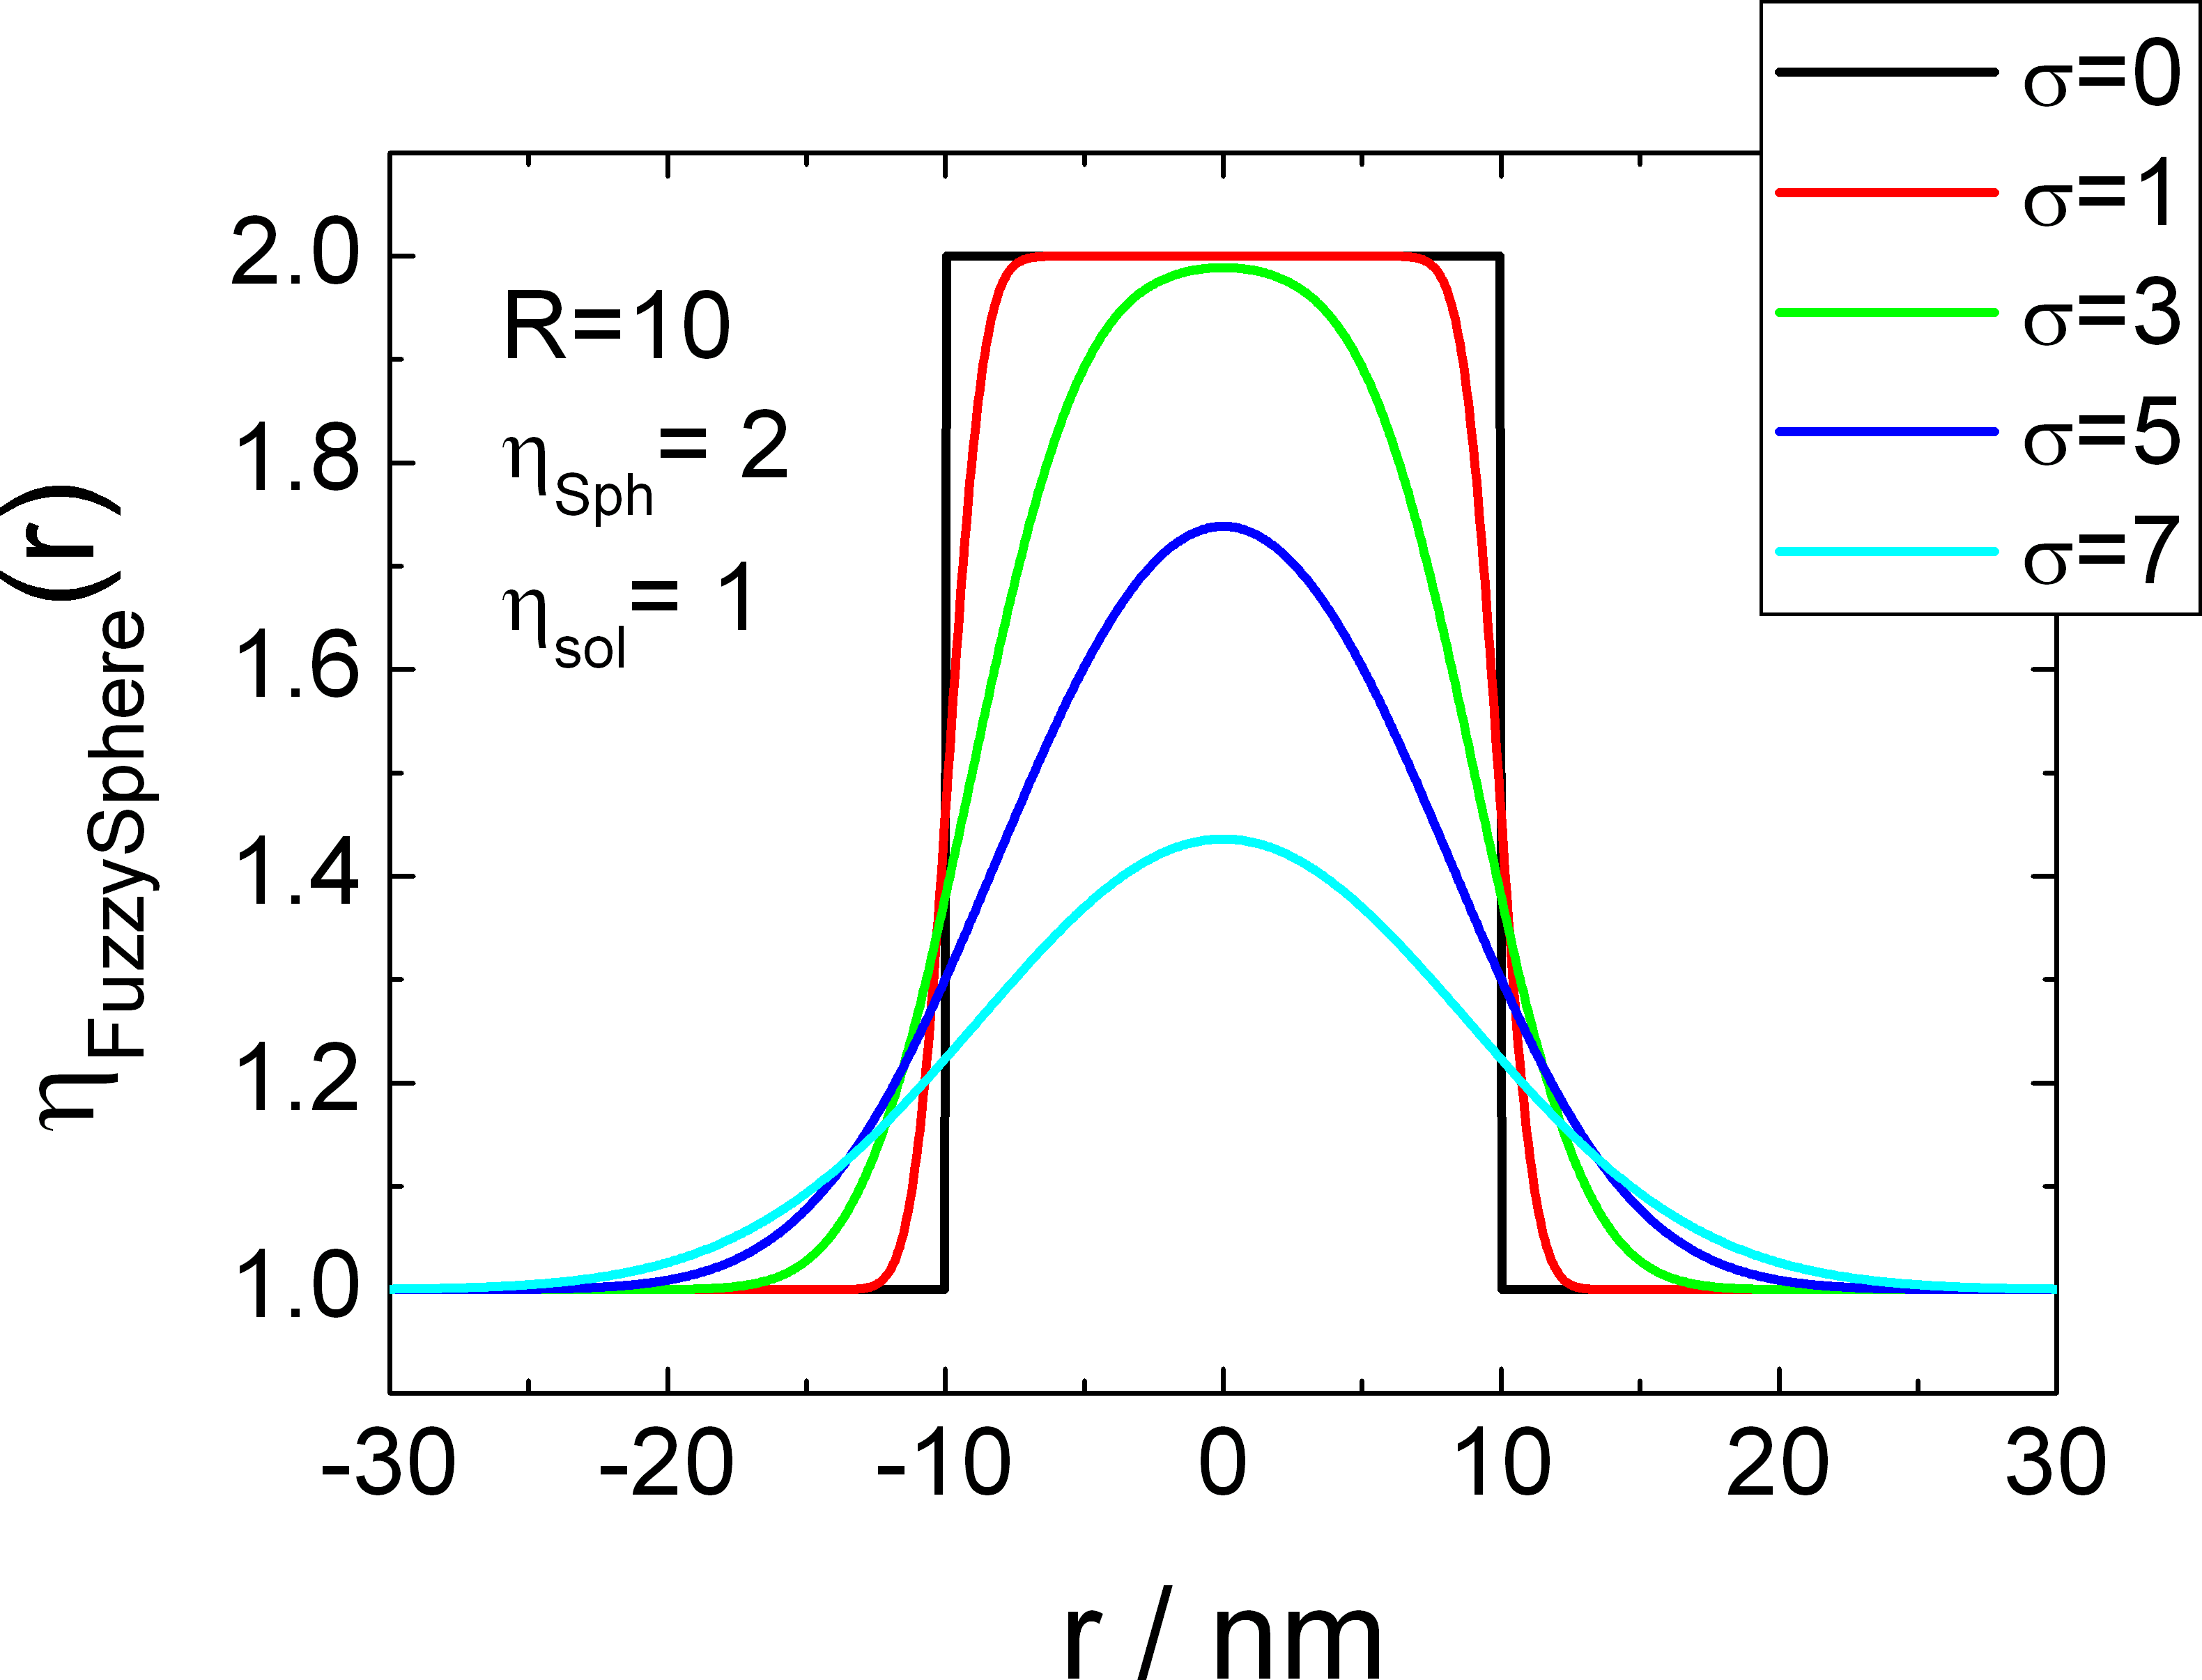
\includegraphics[width=0.7\textwidth,height=0.5\textwidth]{../images/form_factor/FuzzySphere/FuzzySphereProfile.png}
\end{center}
\caption{radial profile of a fuzzy sphere model}
\label{profile:fuzzysphere}
\end{figure}

This model can be used to calculate the scattering from spherical
particles with a "fuzzy" interface \cite{Stieger2004}. The fuzzy
interface is obtained by convoluting the radial profile of a hard
sphere with a Gaussian function.
\begin{align}
\eta_\text{FuzzySph}\left(\abs{\mathbf{r}}\right)
        &= \left(\eta_\text{HS}\star\eta_\text{Gauss}\right)(\mathbf{r}) \nonumber \\
        &= \int_{\mathbb{R}^3}\eta_\text{HS}(\boldsymbol{\tau}) \eta_\text{Gauss}(\mathbf{r}-\boldsymbol{\tau}) d\boldsymbol{\tau}
\end{align}
with
\begin{subequations}
\begin{align}
\eta_\text{HS}\left(\abs{\mathbf{r}}\right) &=
\begin{cases}
\left(\eta_\text{sph}-\eta_\text{sol}\right) & \mbox{for~} \abs{\mathbf{r}}\leq R \\
0 & \mbox{for~} \abs{\mathbf{r}}>R
\end{cases} \\
\eta_\text{Gauss}\left(\abs{\mathbf{r}}\right) &= \frac{1}{2 \sqrt{2} \pi^{3/2}
\abs{\sigma}^3} \exp\left[ -\frac{\abs{\mathbf{r}}^2}{2
\abs{\sigma}^2}\right]
\end{align}
\end{subequations}
The convolution has to be done in $\mathbb{R}^3$. As the hard
sphere and Gaussian functions are radial symmetric also the
profile of the fuzzy sphere only depends on $\abs{\mathbf{r}}$. By
defining the interface via a convolution the form factor can be
easily calculated because the Fourier transform of a convolution
is the pointwise product of the Fourier transforms according to
the convolution theorem, i.e.
\begin{equation}
\begin{split}
F(Q) &= \mathcal{F}\left[\eta_\text{FuzzySph}(r) \right] \\
&=
  \mathcal{F}\left[\left(\eta_\text{HS}\star\eta_\text{Gauss}\right)(r)\right]
= \mathcal{F}\left[\eta_\text{HS}(r)\right] \mathcal{F}\left[\eta_\text{Gauss}(r)\right] \\
%&= \int_0^{\infty} \eta_\text{FuzzySph}(r)\; 4\pi r^2\frac{\sin\left(Qr\right)}{Qr} \; dr \\
&=
   \int_0^{\infty} \eta_\text{HS}(r)\; 4\pi r^2\frac{\sin\left(Qr\right)}{Qr} \; dr \int_0^{\infty} \eta_\text{Gauss}(r)\; 4\pi r^2\frac{\sin\left(Qr\right)}{Qr} \; dr \\
&= \left(\eta_\text{sph}-\eta_\text{sol}\right) 4\pi R^3%8\sqrt{2}\pi^{5/2} R^3
   \frac{\sin\left(QR\right)-QR\cos\left(QR\right)}{\left(QR\right)^3} \quad e^{\left[-\frac{1}{2}\sigma^2Q^2\right]}
\end{split}
\end{equation}

Instead of calculating the convolution integral one also can get
the radial profile of the fuzzy interface by the inverse Fourier
transformation of the scattering amplitude
\begin{align}
\eta_\text{FuzzySph}(r) &= \int_0^{\infty}
\frac{1}{\left(2\pi\right)^3} F(Q) 4\pi Q^2 \frac{\sin\left(Qr\right)}{Qr} \mathrm{d}Q
\end{align}
\begin{multline}
\eta_\text{FuzzySph}(r) = \left(\eta_\text{sph}-\eta_\text{sol}\right) \\
\left( \frac{
    \left(
          e^{-\frac{\left(r + R\right)^2}{2 \sigma^2}}
        - e^{-\frac{\left(r - R\right)^2}{2 \sigma^2}}
    \right) \sigma}{\sqrt{2 \pi} r}
 + \frac{1}{2} \text{erf}\left[\frac{r + R}{\sqrt{2} \abs{\sigma}}\right]
 - \frac{1}{2} \text{erf}\left[\frac{r - R}{\sqrt{2} \abs{\sigma}}\right]
\right)
\end{multline}

Finally the scattering intensity is given by
\begin{multline}
I_\text{FuzzySph}(Q) = F^2(Q) = \\
\left[ \left(\eta_\text{sph}-\eta_\text{sol}\right) 4\pi R^3
   \frac{\sin\left(QR\right)-QR\cos\left(QR\right)}{\left(QR\right)^3} \quad e^{\left[-\frac{1}{2}\sigma^2Q^2\right]}
\right]^2
\end{multline}

The intensity $I_\text{FuzzySph}(Q)$ and also the scattering
length density profile $\eta_\text{FuzzySph}(r)$ are normalized so that
\begin{align*}
 \lim_{Q \to 0} I_\text{FuzzySph}(Q) &= \left( \left(\eta_\text{sph}-\eta_\text{sol}\right) \frac{4}{3}\pi R^3\right)^2 \\
 \int_0^{\infty} 4\pi r^2 \; \eta_\text{FuzzySph}(r) \; \mathrm{d}r &=\frac{4}{3}\pi R^3
\end{align*}

\begin{align}
R &=\text{radius of the fuzzy sphere} \nonumber\\
\sigma &=\text{thickness of the fuzzy shell} \nonumber\\
\eta_\text{sph}   & : \text{scattering length density of sphere} \nonumber \\
\eta_\text{sol}   & : \text{scattering length density of the solvent} \nonumber \\
%I_\text{fluct}    & : \text{forward scattering of the internal fluctuation contribution} \nonumber \\
%\xi               & : \text{correlation length of the fluctuations} \nonumber
\end{align}


\vspace{5mm}

\hspace{1pt}\\
\underline{Input Parameters for model \texttt{FuzzySphere} and \texttt{radial profile of FuzzySphere}:}\\
\begin{description}
\item[\texttt{R}] radius of the fuzzy sphere  $R$
\item[\texttt{sigma}] thickness of the fuzzy shell $\sigma$
\item[\texttt{eta\_sph}] scattering length density of sphere
$\eta_\text{sph}$ \item[\texttt{eta\_sol}] scattering length
density of solvent $\eta_\text{sol}$
%\item[\texttt{I\_fluct}] forward scattering of the internal fluctuation contribution $I_\text{fluct}$
%\item[\texttt{xi}] correlation length of the fluctuations $\xi$
\end{description}

\noindent\underline{Note:}
\begin{itemize}
\item This form factor is only defined for positive radii $R>0$.
\item For $\sigma = 0$ the limiting case of a simple hard sphere
form factor is used.
\item In addition, scattering contributions
arising from fluctuations of the microgel network are often
included in this model expression as a Lorentzian function
\begin{align}
I_\text{fluct}(Q) &= \frac{I_\text{fluct}(0)}{1+\xi^2Q^2}
\end{align}
so that
\begin{align}
I(Q) &= I_\text{FuzzySph}(Q)+I_\text{fluct}(Q)
\end{align}
where $I_\text{fluct}(0)$ is the $Q=0$ limiting intensity and
$\xi$ represents the correlation length of the fluctuations, which
can be considered to be related to the blob or mesh size. It
should be noted that the Lorentzian describes the ensemble average
correlations in the polymer network.

\end{itemize}

\begin{figure}[htb]
\begin{center}
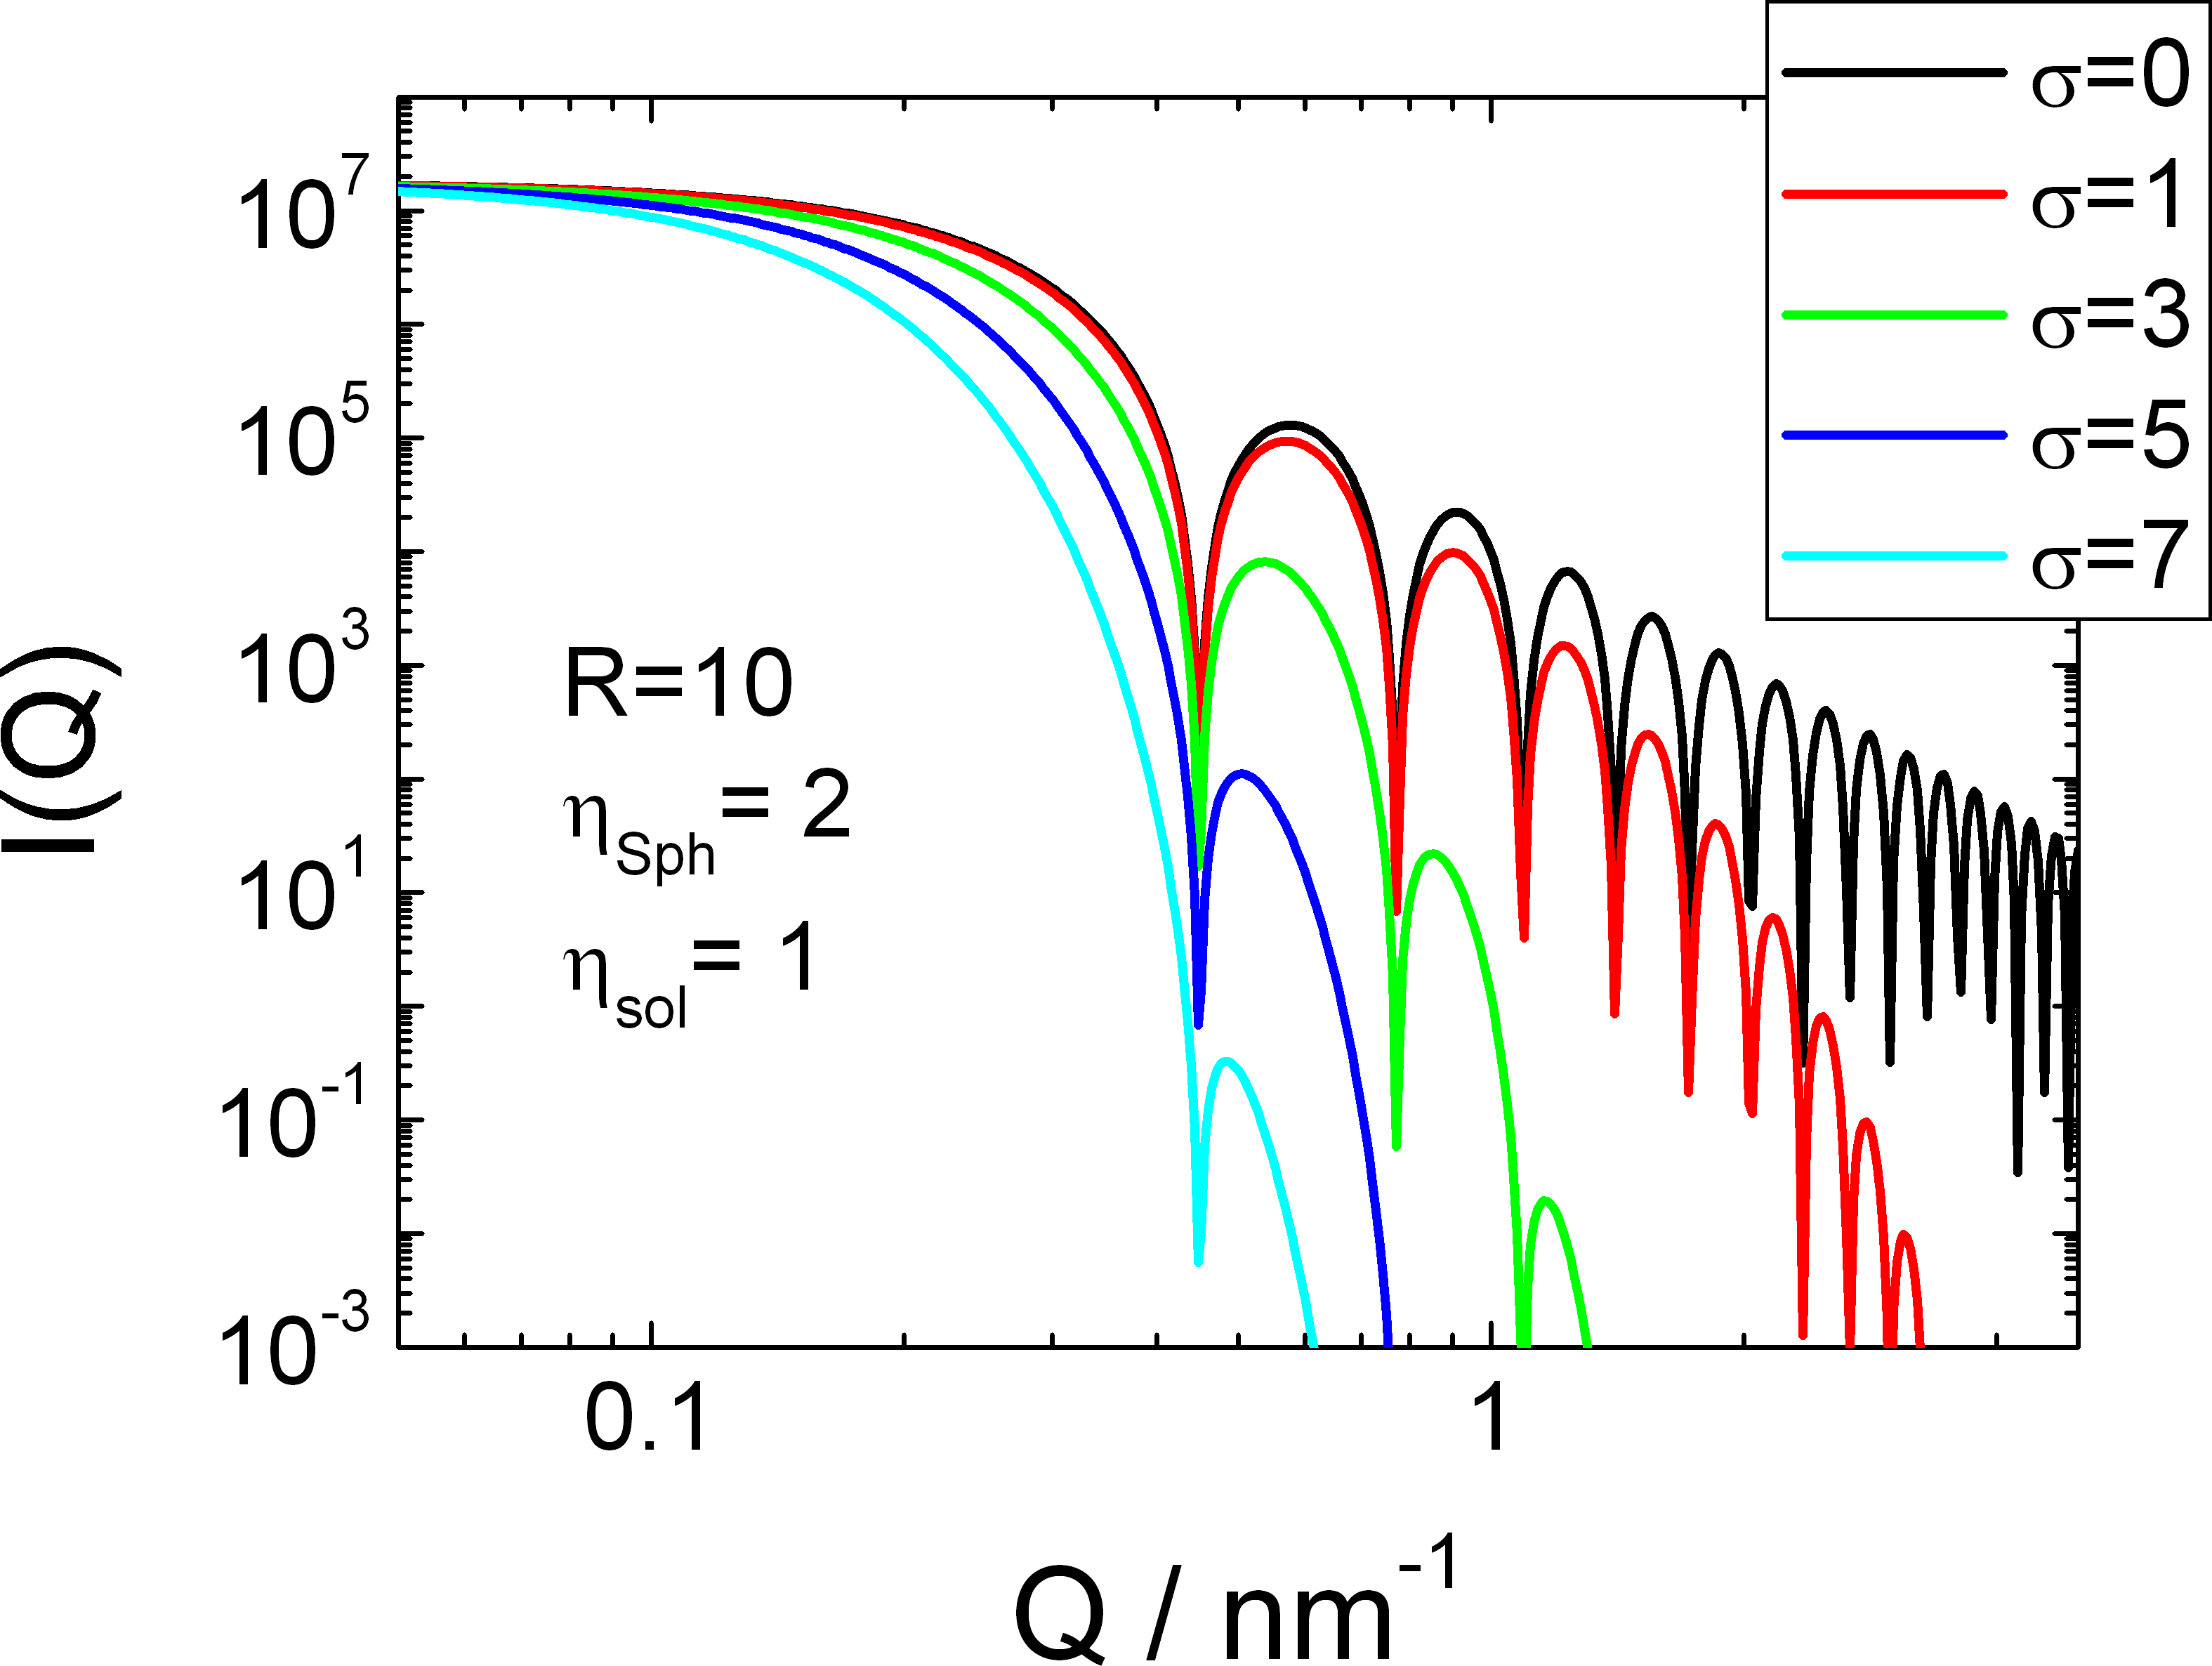
\includegraphics[width=0.7\textwidth,height=0.5\textwidth]{../images/form_factor/FuzzySphere/FuzzySphereIQ.png}
\end{center}
\caption{Scattering intensity of a fuzzy sphere. The scattering
intensity has been calculated for a core radius $R=10$, a
scattering length density of the FuzzySphere of
$\eta_\text{Sph}=1$, a scattering length density of the solvent
$\eta_\text{sol}=1$, and several widths of the "fuzzy" shell}
\label{fig:I_FuzzySphere}
\end{figure}

%%%%%%%%%%%%%%%%%%%%%%%%%%%%%%%%%%%%%%%%%%%%%%%%%%%%%%%%%%%%%%%%%%%%%%%%

\clearpage
\subsection{CoreShellMicrogel}
\label{sect:CoreShellMicrogel}

\begin{figure}[htb]
\begin{center}
\subfigure[radial profile of a sphere with a parabolic interface]{
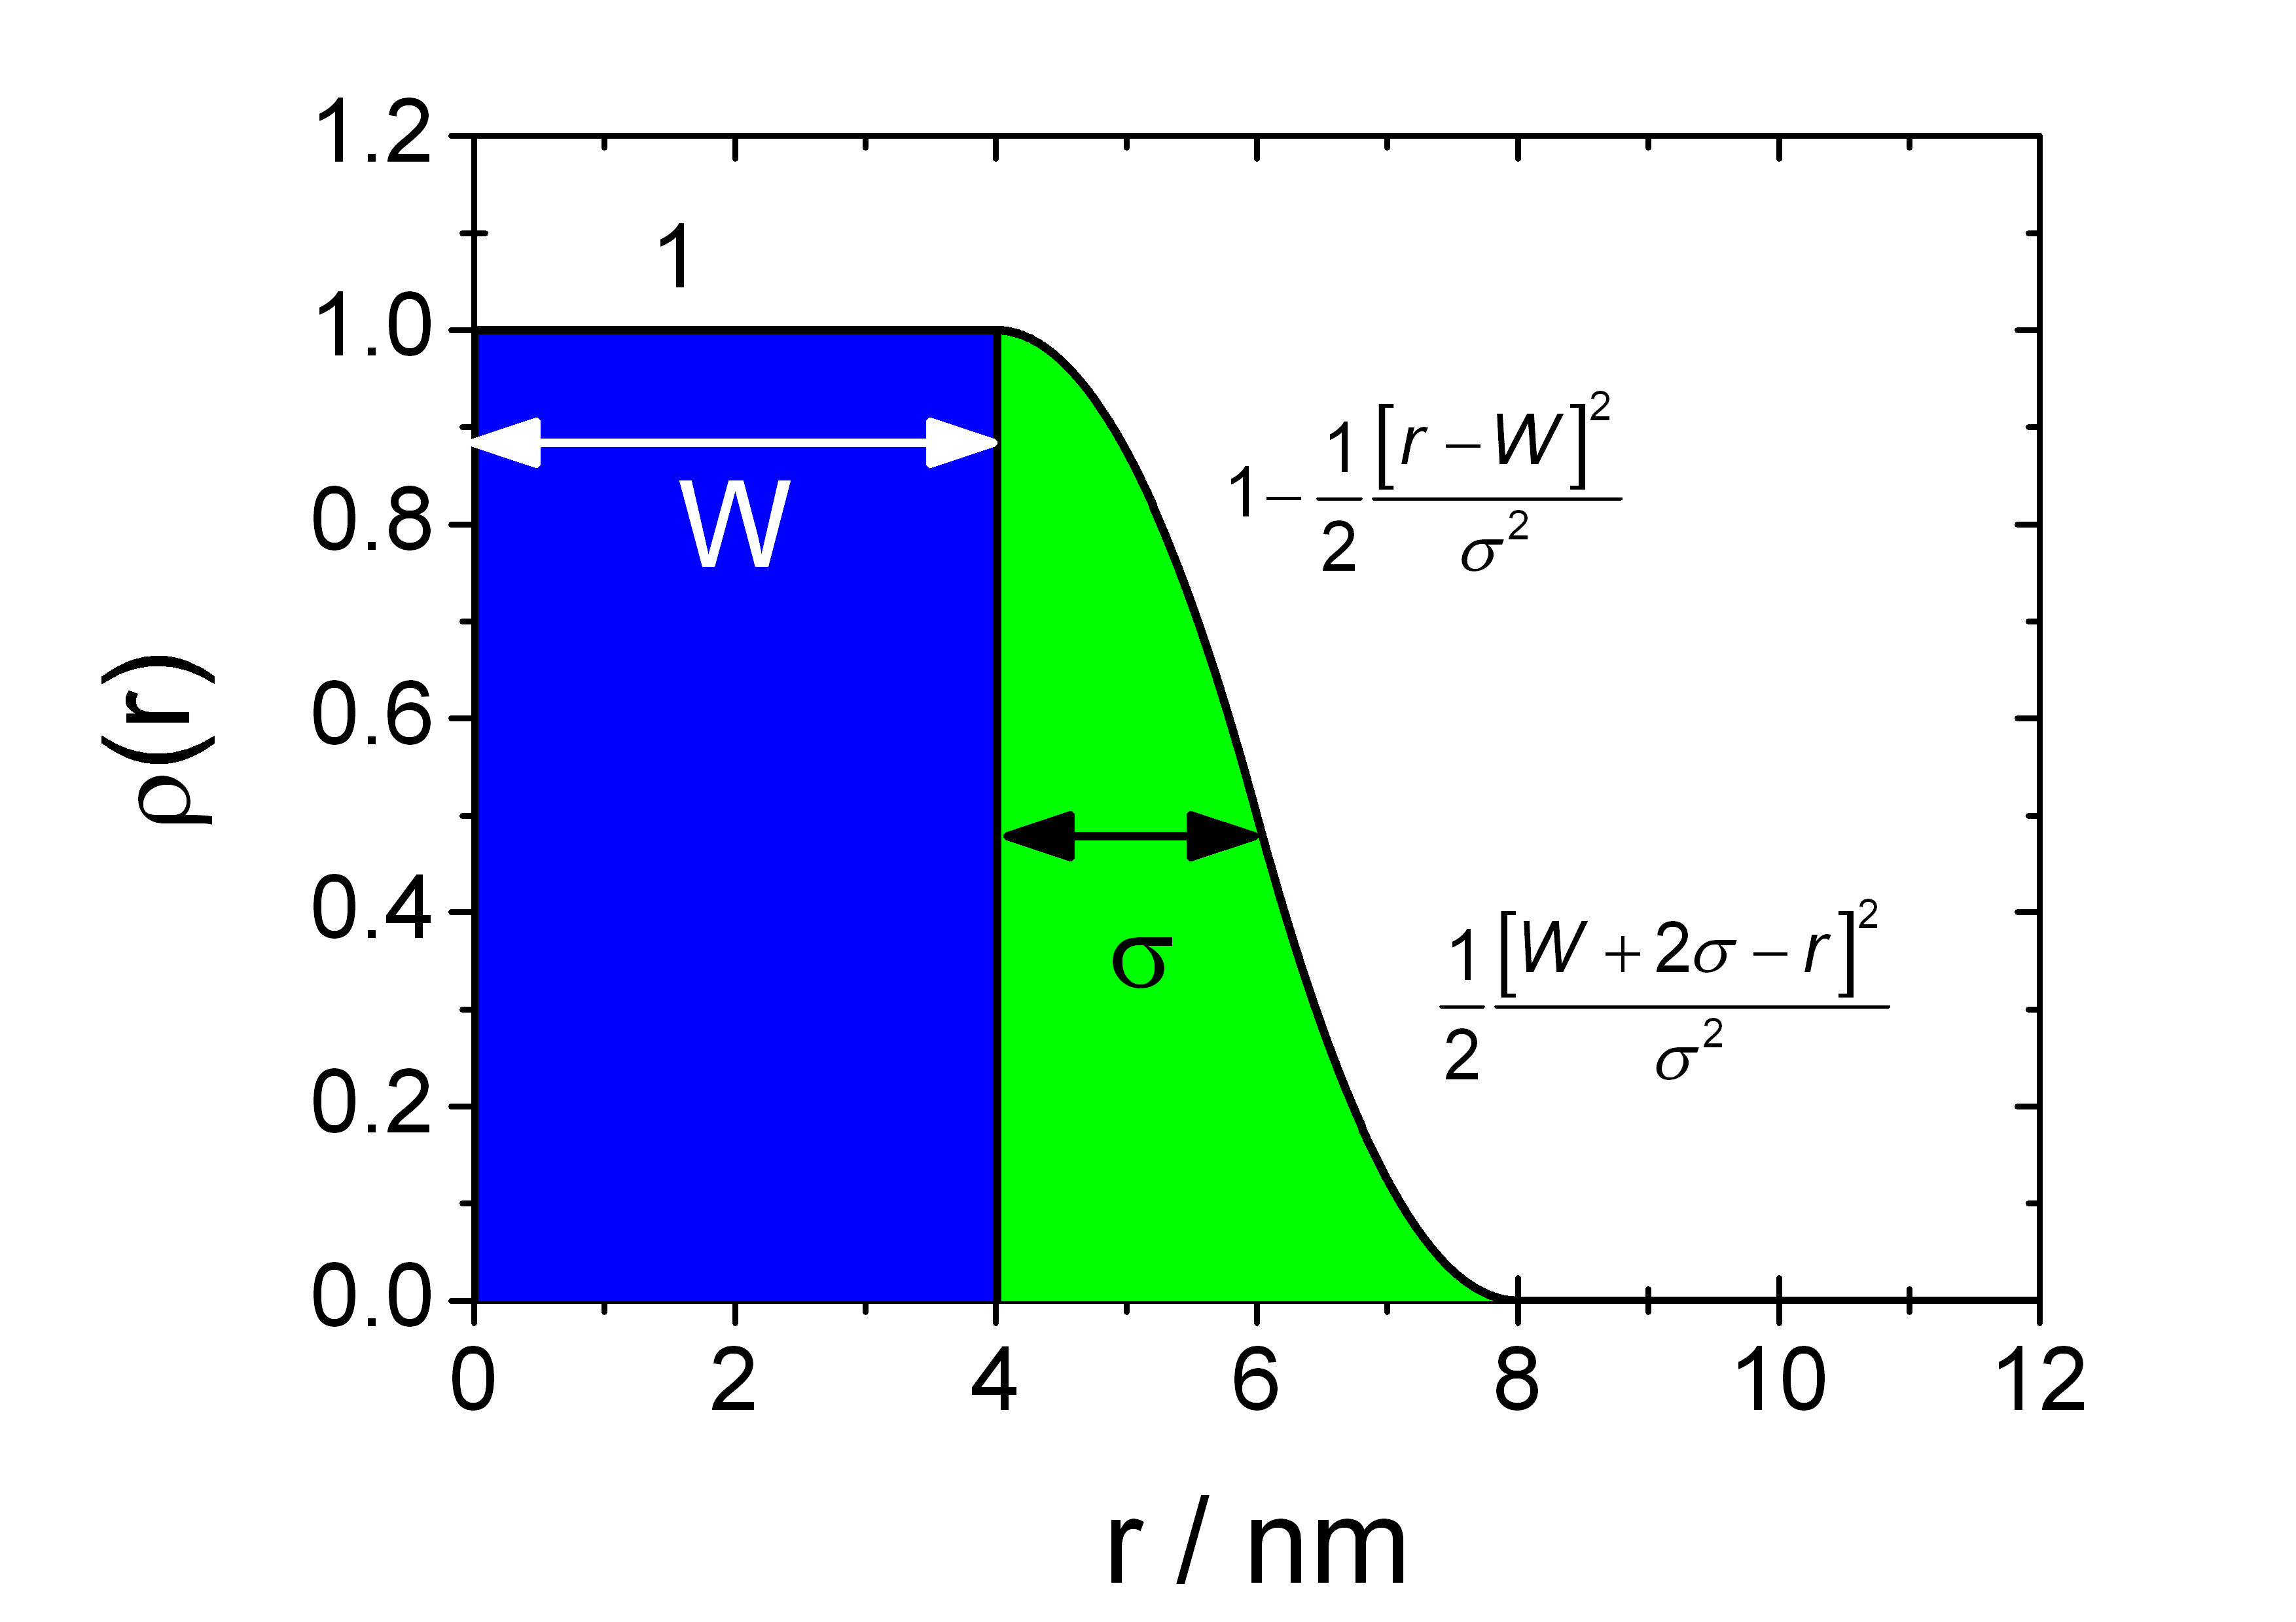
\includegraphics[width=0.48\textwidth,height=0.35\textwidth]{../images/form_factor/FuzzySphere/CoreShellMicrogel1.png}}
\hfill
\subfigure[radial profile of a spherical shell with parabolic interfaces]{
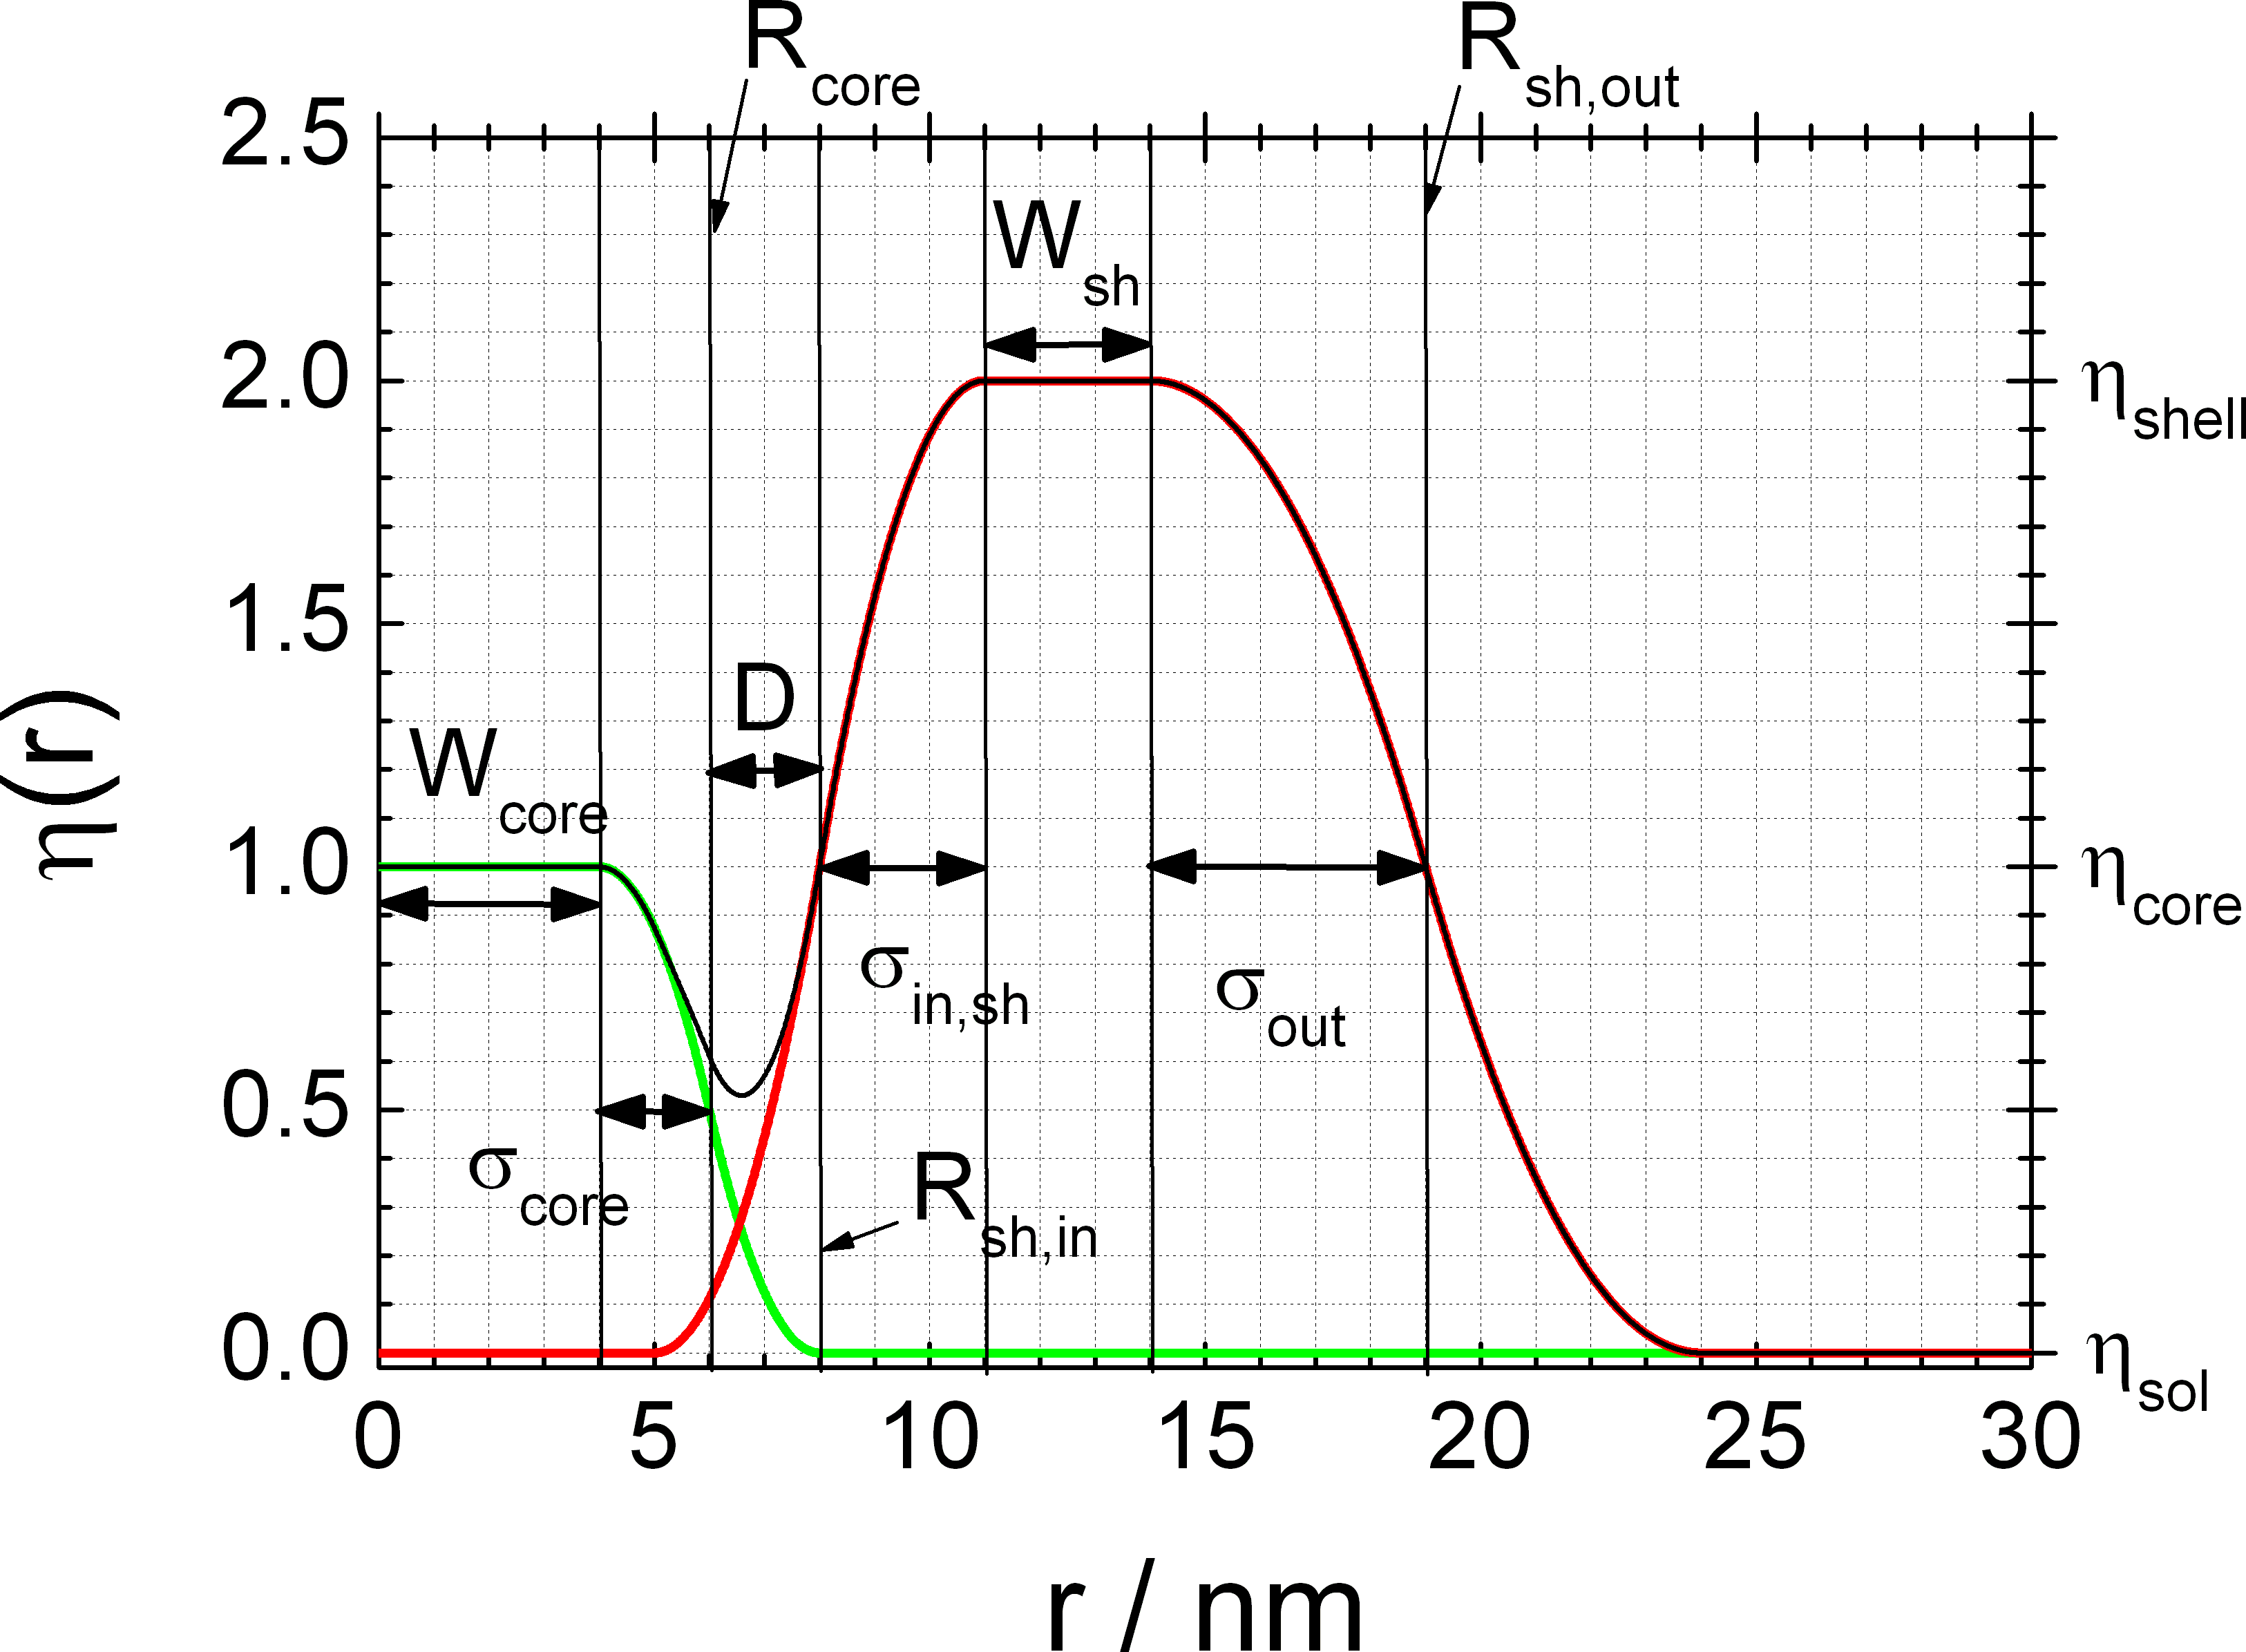
\includegraphics[width=0.48\textwidth,height=0.35\textwidth]{../images/form_factor/FuzzySphere/CoreShellMicrogel2.png}}
\end{center}
\caption{.....}
\label{fig:profile:CoreShellMicrogel}
\end{figure}


This model can be used to calculate the scattering from spherical
particles with a parabolic "fuzzy" interface \cite{Berndt2005,Berndt2006,Berndt2006a}.
The radial profile is given by
\begin{align}
\rho(r,R,\sigma) &=
\begin{cases}
1 & \mbox{for } r\leq R-\sigma \\
1-\frac{1}{2}\frac{\left((r-R)+\sigma\right)^2}{\sigma^2} & \mbox{for } R-\sigma < r \leq R \\
\frac{1}{2}\frac{\left((R-r)+\sigma\right)^2}{\sigma^2} & \mbox{for } R< r\leq R+\sigma \\
0 & \mbox{for } r > \leq R+\sigma
\end{cases}
\label{eq:CoreShellMicrogelProfile}
\end{align}
where $R=W+\sigma$. For such a radial profile the Fourier-transformation can be calculated analytically as
\begin{multline}
F(Q,R,\sigma) = \mathcal{F}[\rho(r,R,\sigma)] = \\
4 \pi \Bigg(
        \left(\frac{R}{\sigma^2}+\frac{1}{\sigma}\right) \frac{\cos (q(R+\sigma))}{q^4}
    +   \left(\frac{R}{\sigma^2}-\frac{1}{\sigma}\right) \frac{\cos (q(R-\sigma))}{q^4} \\
    -   3 \frac{\sin(q(R+\sigma))}{q^5 \sigma^2}
    -   3 \frac{\sin(q(R-\sigma))}{q^5 \sigma^2}
    -   6  \frac{\sin(qR)}{q^5 \sigma^2}
    -   2 R \frac{\cos(qR)}{q^4 \sigma^2}
\Bigg)
\end{multline}
The last term in the brackets needed to be corrected compared to the papers mentioned above
due to a typo in the original papers.
The radial scattering length density profile of a fuzzy core
shell like in Fig.\ \ref{fig:profile:CoreShellMicrogel}b can be obtained by
\begin{multline}
\eta_{core,sh}(r,W_\textrm{core},\sigma_\textrm{core},D,\sigma_\textrm{sh,in},W_\textrm{sh},\sigma_\textrm{sh,out}) =
    \eta_\textrm{sol}
+ (\eta_\textrm{shell}-\eta_\textrm{sol}) \rho(r,R_\textrm{out},\sigma_\textrm{out}) \\
+ (\eta_\textrm{shell}-\eta_\textrm{sol}) \rho(r,R_\textrm{sh,in},\sigma_\textrm{sh,in})
+ (\eta_\textrm{core} -\eta_\textrm{sol}) \rho(r,R_\textrm{core},\sigma_\textrm{core})
\end{multline}
with
\begin{subequations}
\begin{align}
    R_\textrm{core} &= W_\textrm{core}+\sigma_\textrm{core} \\
    R_\textrm{sh,in}&= R_\textrm{core}+D \\
    R_\textrm{out}  &= R_\textrm{sh,in}+\sigma_\textrm{sh,in}+W_\textrm{sh}+\sigma_\textrm{sh,out}
\end{align}
\label{eq:radiiCoreShellMicrogel}
\end{subequations}
In the same way also the scattering amplitude $F_\textrm{core,sh}(Q,\cdots)$ and the scattering intensity
$I_\textrm{core,sh}(Q,\cdots)=\abs{F_\textrm{core,sh}(Q,\cdots)}^2$ can be calculated
\begin{subequations}
\begin{multline}
F_\textrm{core,sh}(Q,W_\textrm{core},\sigma_\textrm{core},D,\sigma_\textrm{sh,in},W_\textrm{sh},\sigma_\textrm{sh,out}) =
  (\eta_\textrm{shell}-\eta_\textrm{sol}) F(Q,R_\textrm{out},\sigma_\textrm{out}) \\
+ (\eta_\textrm{shell}-\eta_\textrm{sol}) F(Q,R_\textrm{sh,in},\sigma_\textrm{sh,in})
+ (\eta_\textrm{core} -\eta_\textrm{sol}) F(Q,R_\textrm{core},\sigma_\textrm{core})
\end{multline}
\begin{align}
I_\textrm{core,sh}(Q,W_\textrm{core},\sigma_\textrm{core},D,\sigma_\textrm{sh,in},W_\textrm{sh},\sigma_\textrm{sh,out}) &=
\abs{F_\textrm{core,sh}(Q,\cdots)}^2
\end{align}
\end{subequations}

\vspace{5mm}

\noindent
\textbf{Input parameters for "\texttt{CoreShellMicrogel}" and "\texttt{radial profile of CoreShellMicrogel}":}
\begin{description}
    \item[\texttt{W\_core}] radius of center parts of core $W_\textrm{core}$ with homogeneous scattering length density
    \item[\texttt{sigma\_core}] interface half width of the core $\sigma_\mathrm{core}$
    \item[\texttt{W\_shell}] width of center parts of shell $W_\textrm{sh}$ with homogeneous scattering length density
    \item[\texttt{sigma\_sh,in}] half width of the inner interface of shell $\sigma_\mathrm{sh,in}$
    \item[\texttt{D}] distance $D$ between interface of core and in interface of shell
    \item[\texttt{sigma\_out}] half width of the outer surface profile $\sigma_\mathrm{out}$
    \item[\texttt{eta\_core}] scattering length density of homogeneous core part $\eta_\textrm{core}$
    \item[\texttt{eta\_shell}] scattering length density of homogeneous shell part $\eta_\textrm{shell}$
    \item[\texttt{eta\_sol}] scattering length density of solvent $\eta_\textrm{sol}$
\end{description}

\noindent
\textbf{Note}
\begin{itemize}
  \item If one like to simulate a simple step profile one should set $D=0$ and
        $\sigma_\mathrm{core}=\sigma_\mathrm{sh,in}$. The last equality
        in case of fitting this parameter can be simply obtained by a global parameter
        under fitting multiple data sets.
  \item Instead of using the radii in eq.\ \ref{eq:radiiCoreShellMicrogel} as input parameters the thickness
        of the homogeneous parts of the core and the shell have been used to avoid a problems
        (negative dimensions) by applying an integration over a size distribution starting from 0 on the radii.
\end{itemize}
\begin{figure}[htb]
\begin{center}
\subfigure[Some radial profiles of spheres with a parabolic interfaces  which have been used to calculate the scattering curve in Fig.\ (b).
]{
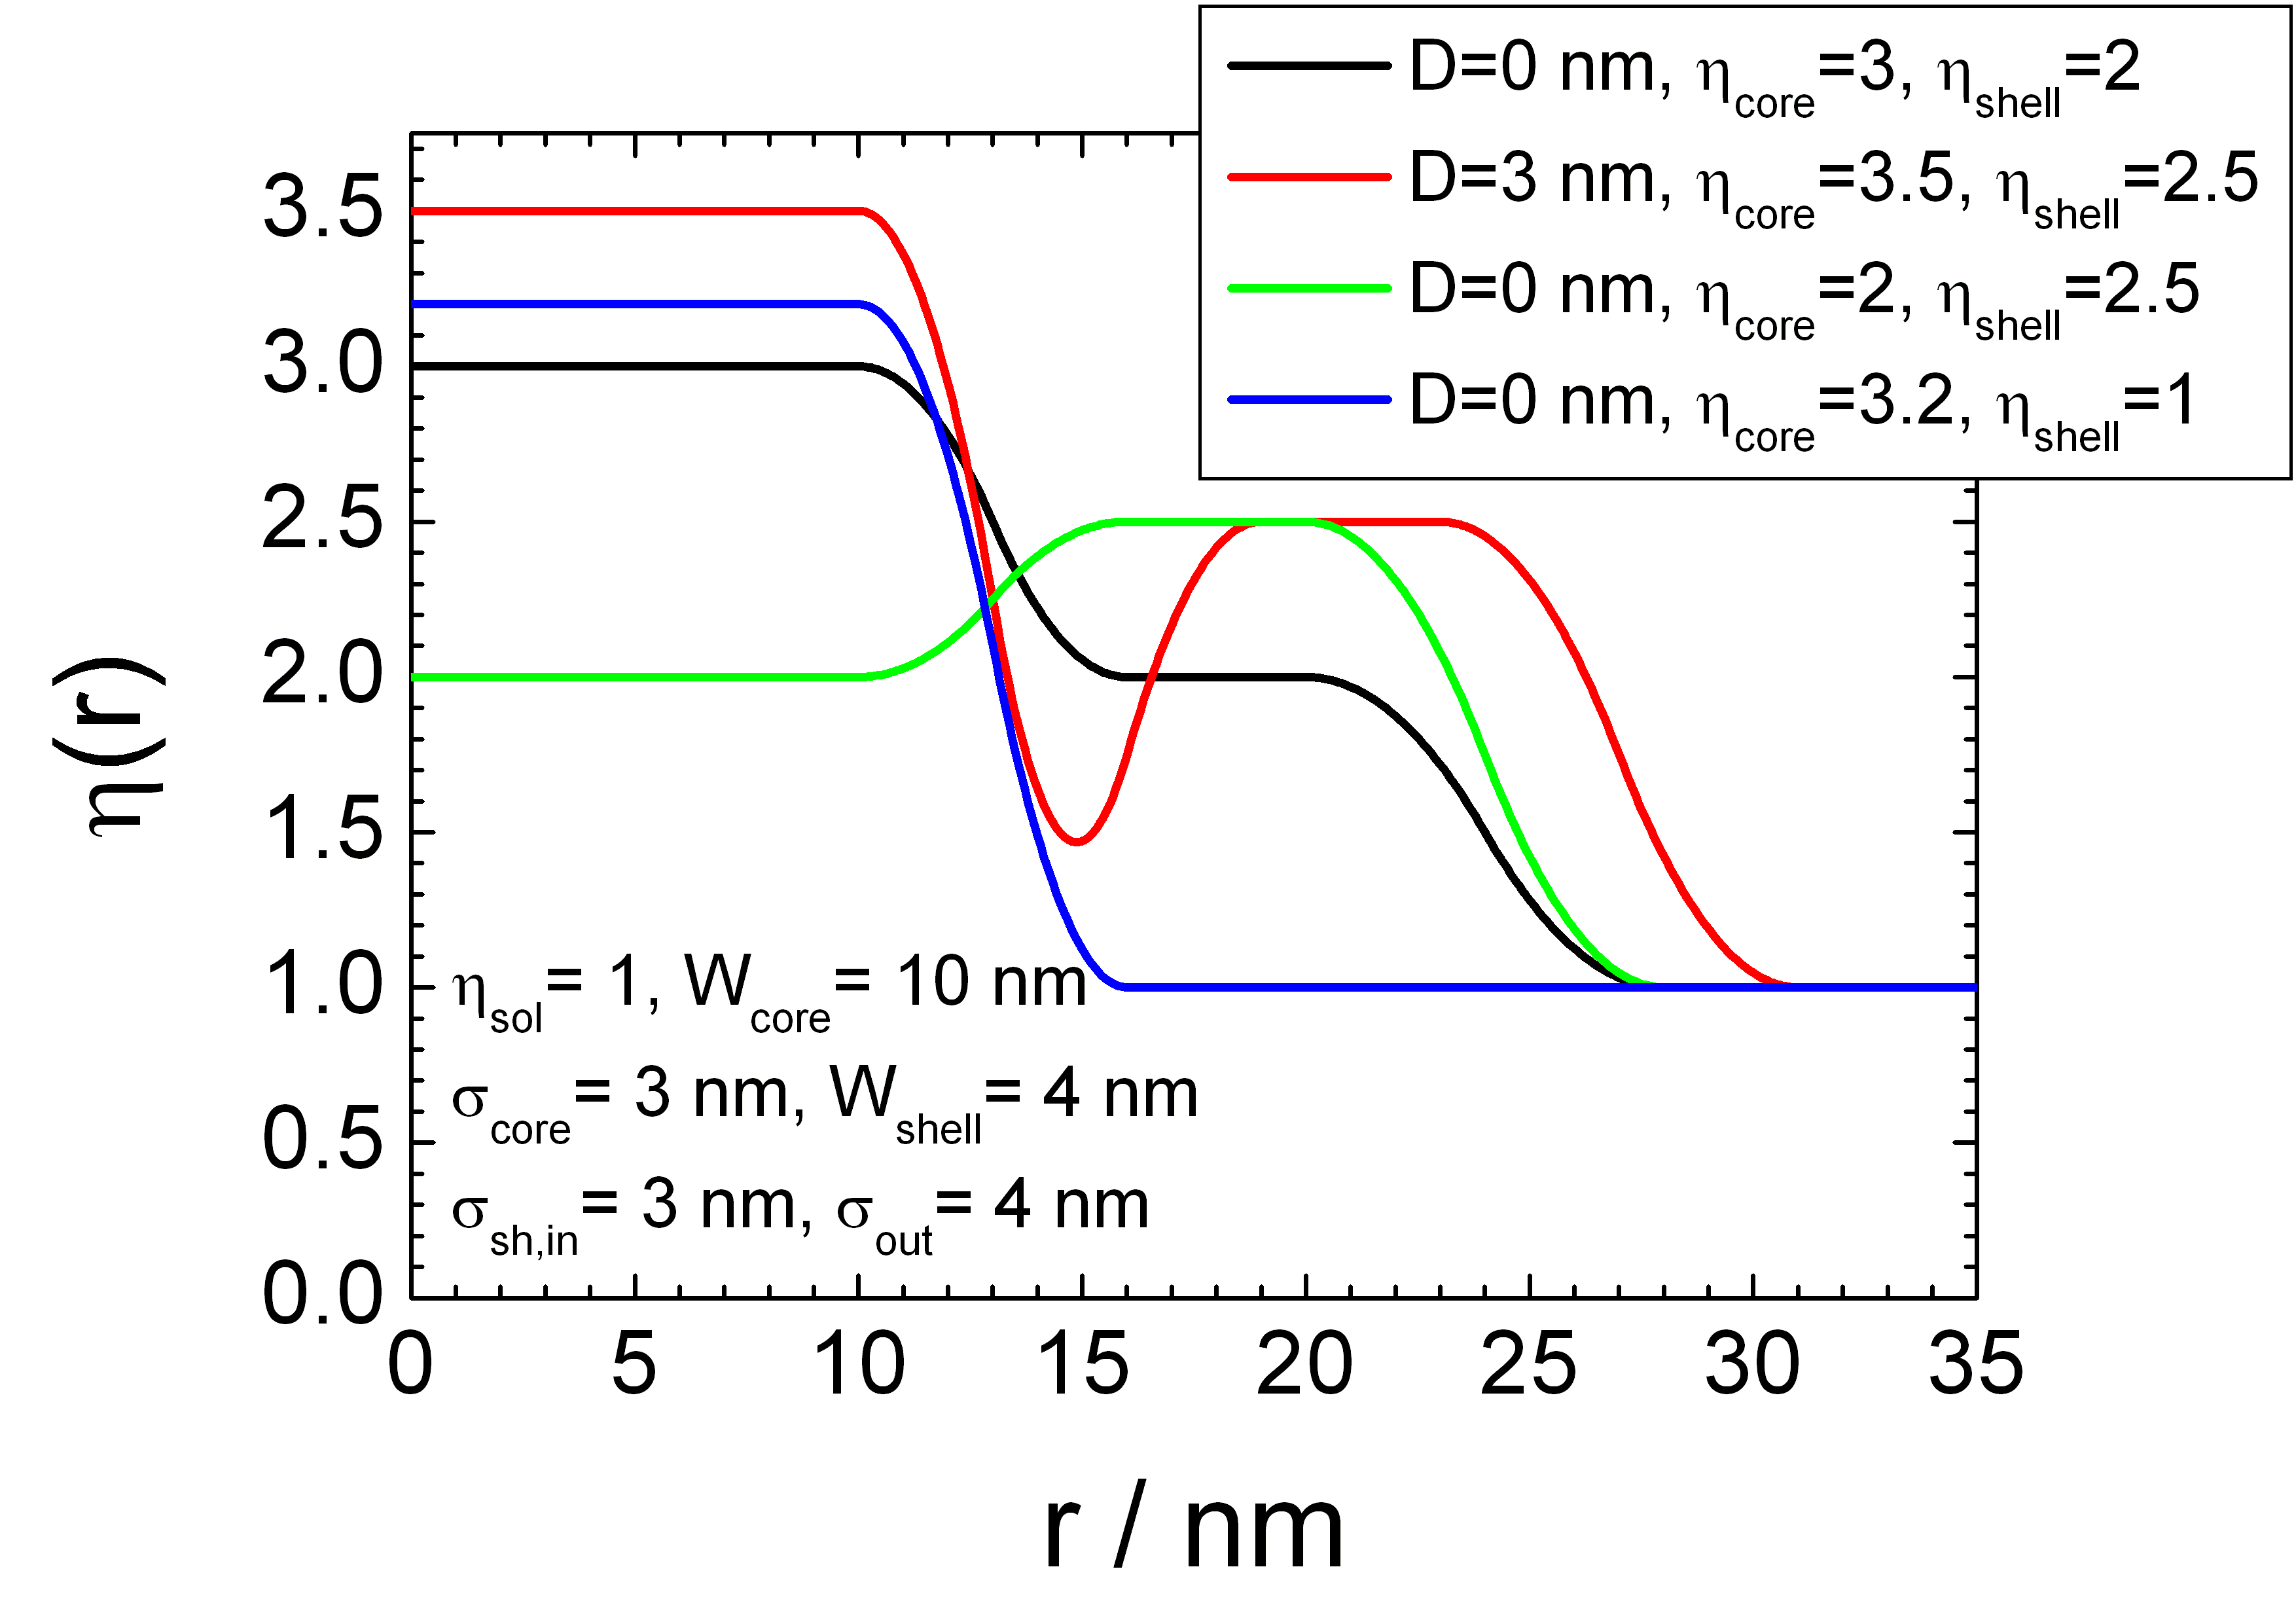
\includegraphics[width=0.48\textwidth,height=0.35\textwidth]{../images/form_factor/FuzzySphere/Example_CoreShellMicrogel1.png}}
\hfill
\subfigure[Scattering curves of the radial profiles shown in Fig.\ (a).]{
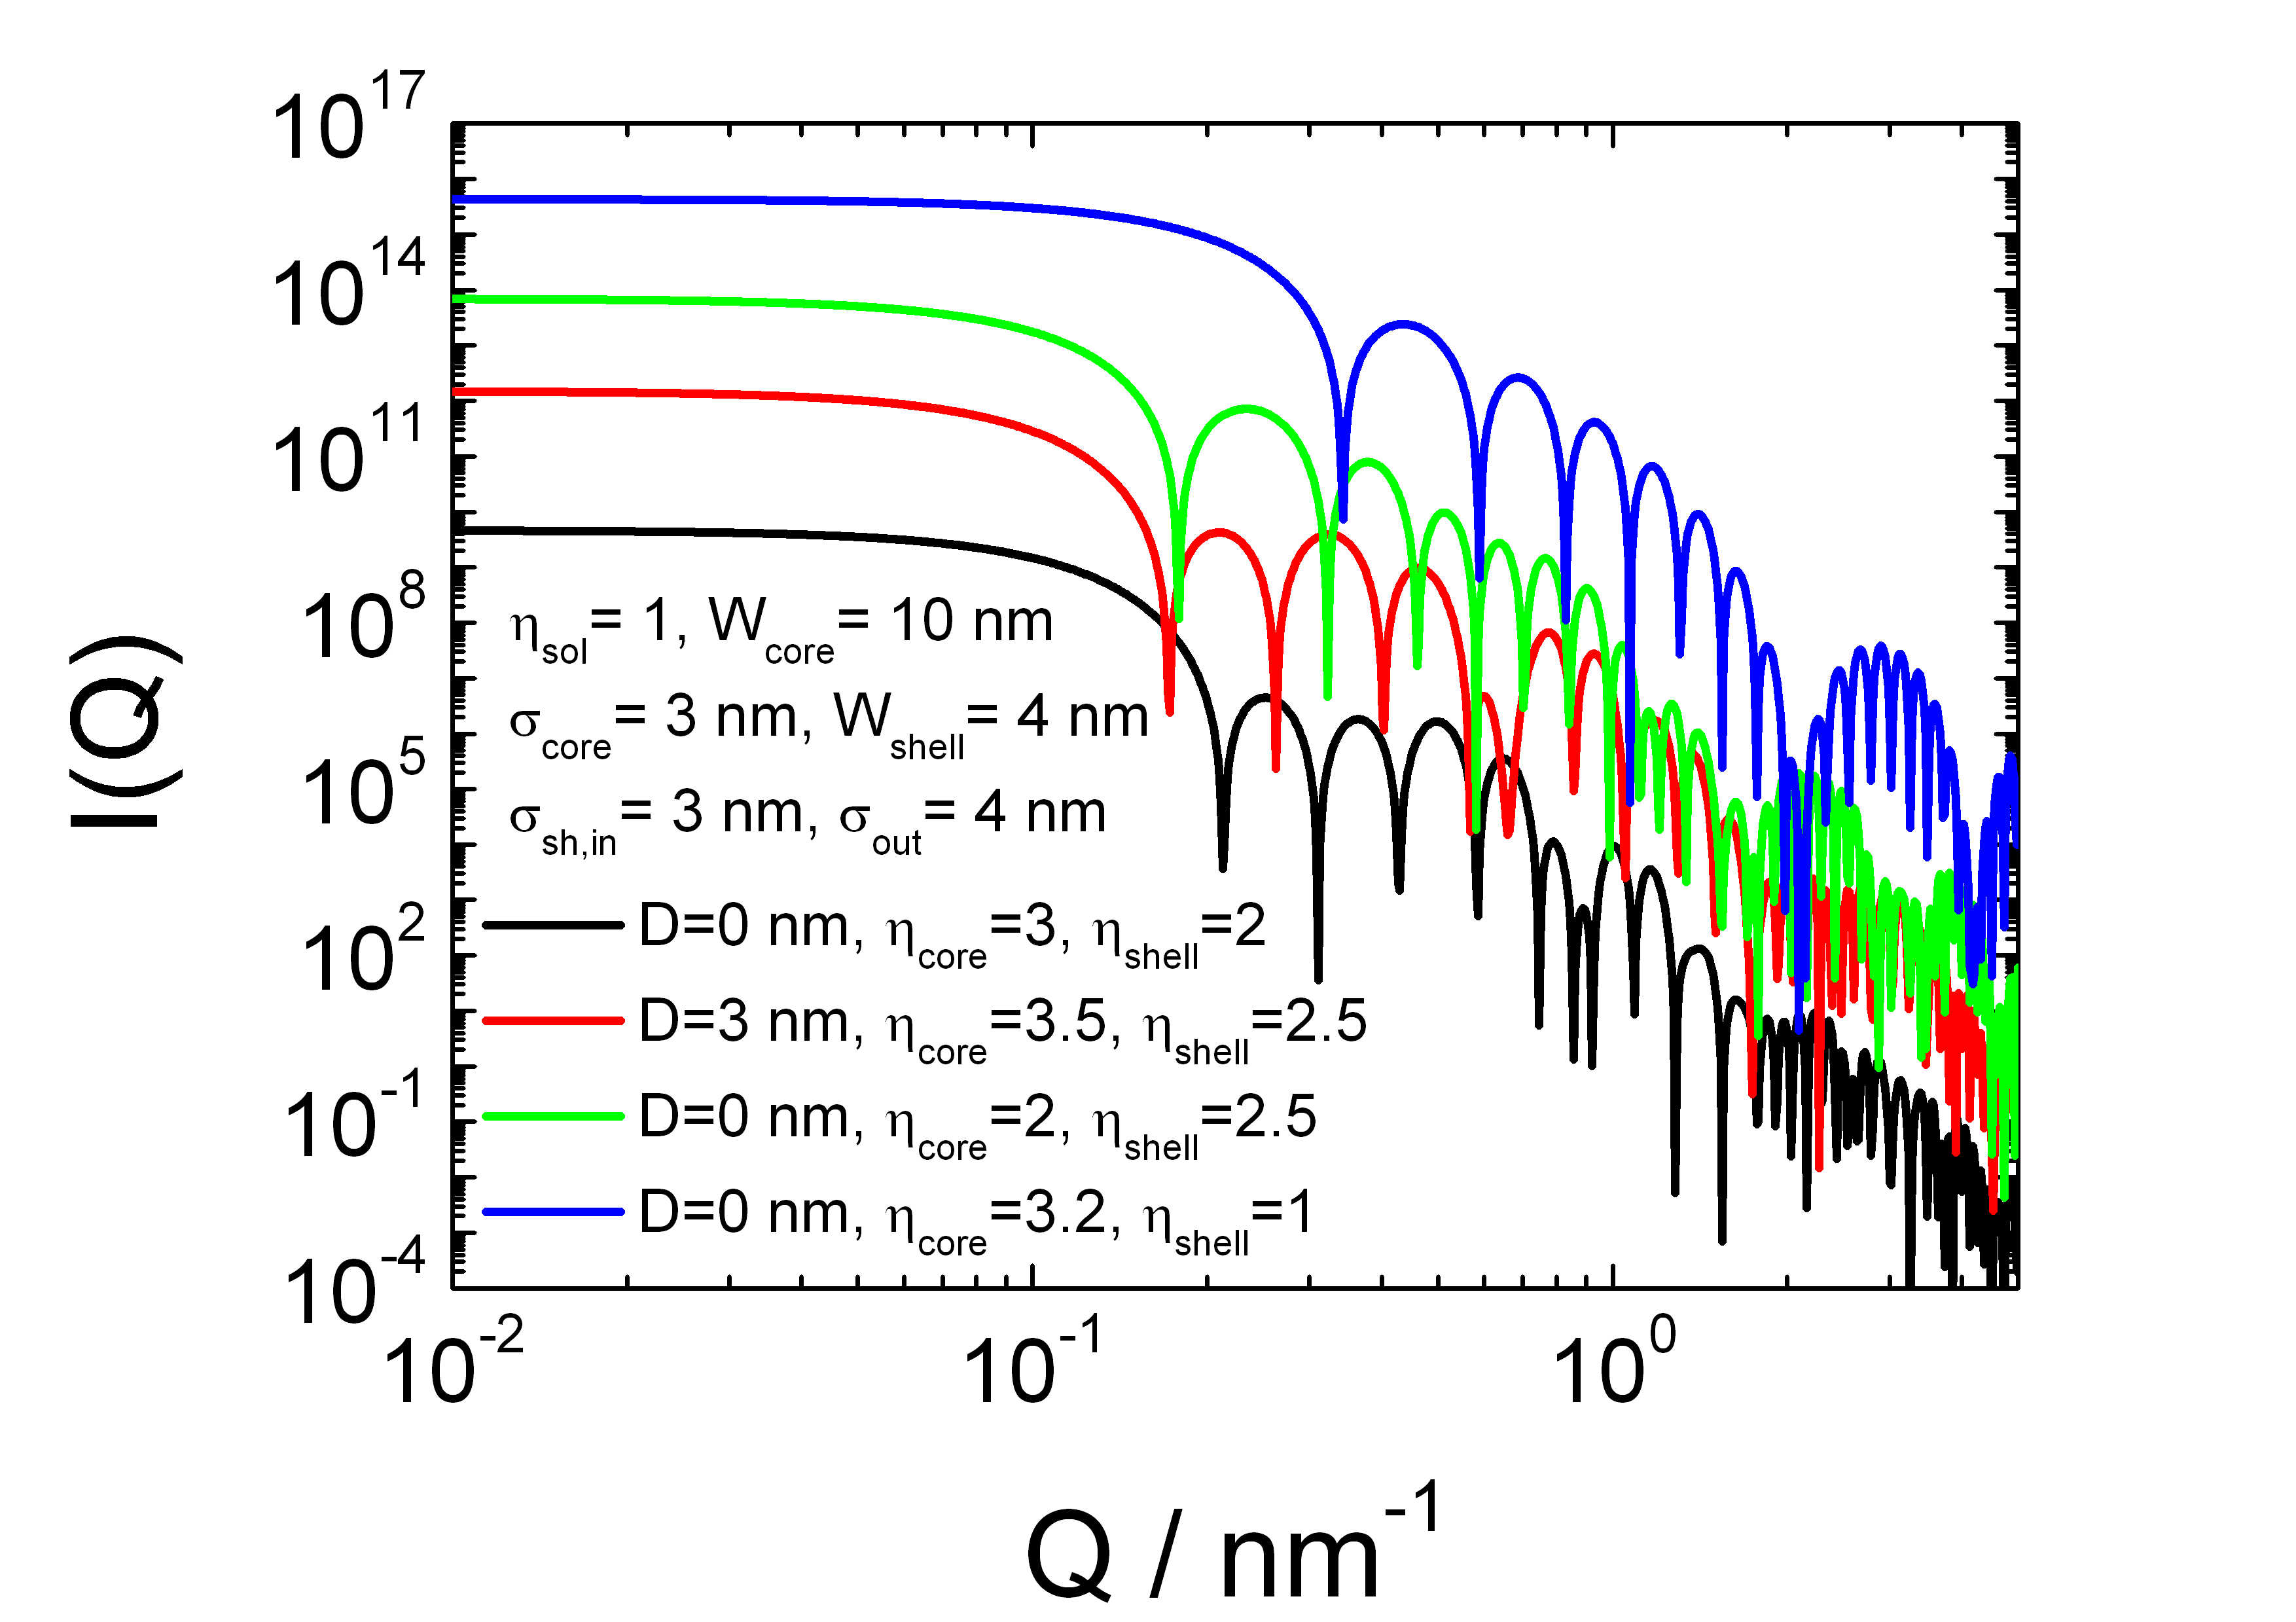
\includegraphics[width=0.48\textwidth,height=0.35\textwidth]{../images/form_factor/FuzzySphere/Example_CoreShellMicrogel2.png}}
\end{center}
\caption{The profiles and scattering curves hve been calculated with the plugin functions
"\texttt{CoreShellMicrogel}" and "\texttt{Radial Profile of CoreShellMicrogel}".}
\label{fig:profile:Example_CoreShellMicrogel}
\end{figure}

%%%%%%%%%%%%%%%%%%%%%%%%%%%%%%%%%%%%%%%%%%%%%%%%%%%%%%%%%%%%%%%%%%%%%%%%%%%%%%%%

\clearpage
\subsection{Spherical shell with linear varying contrast profile (LinShell)}
\label{sect:LinShell} ~\\

\begin{figure}[htb]
\begin{center}
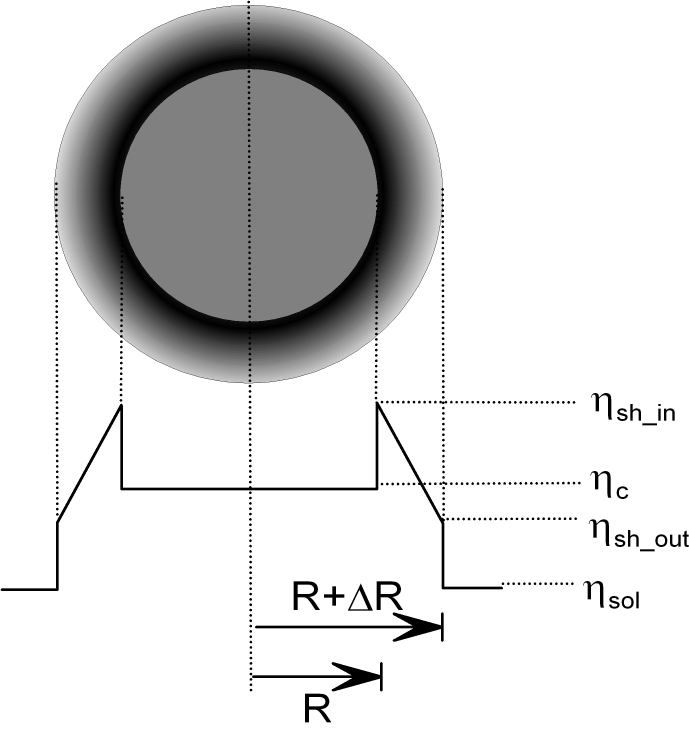
\includegraphics[width=0.5\textwidth,height=0.533\textwidth]{../images/form_factor/spheres/linshell.png}
\end{center}
\caption{Radial profile for calculating the form factor of a spherical shell with a core radius $R$
and a shell thickness of $\Delta R$ and a linear varying contrast
profile.} \label{LinShell1Profile}
\end{figure}

Form factor of a spherical shell with a core radius $R$ and a
shell thickness of $\Delta R$. Here a linear contrast profile
within the shell has been assumed.

\begin{align}
\Delta\eta(r)      & =
\begin{cases}
\eta_\text{c} & \text{~for~} r<R \\
m r + b  & \text{~for~} r \in [R,R+\Delta R] \\
\eta_\text{sol}  & \text{~for~} r>R+\Delta R
\end{cases}\\
m           & = (\eta_\text{sh\_out}-\eta_\text{sh\_in}) / \Delta R \\
b           & = -m R + \eta_\text{sh\_in} \\
\eta_\text{sh\_in}  & = (1 - x_\text{in,sol})  \, \eta_\text{sh} + x_\text{in,sol} \,\eta_\text{sol}-\eta_\text{sol} \\
                    & : \text{scattering length density at $R$} \nonumber \\
\eta_\text{sh\_out} & = (1 - x_\text{out,sol}) \, \eta_\text{sh} + x_\text{out,sol}\,\eta_\text{sol}-\eta_\text{sol} \\
                    & : \text{scattering length density at $R+\Delta R$} \nonumber \\
\eta_\text{sh}      & : \text{scattering length density of pure shell material} \nonumber \\
\eta_\text{c}       & : \text{scattering length density of core} \nonumber \\
\nonumber
\end{align}

\begin{align}
F_\text{sph}(A,x) & = \frac{4}{3}\pi x^3 \,\, 3\frac{\sin(A)-A\cos(A)}{A^3} \\[5mm]
F_\text{shlin}(A,x) & = 4\pi x^4 \frac{2\cos(A)+2A\sin(A)-A^2\cos(A)}{A^4} \\[5mm]
I_\text{LinShell}    & = \big[ \,\, (\eta_\text{c}-\eta_\text{sol}-b)F_\text{sph}(QR,R) \nonumber \\
             & \hspace{6mm} - mF_\text{shlin}(QR,R) \\
             & \hspace{6mm} + mF_\text{shlin}\left(Q(R+\Delta R),R+\Delta R\right) \nonumber \\
             & \hspace{6mm} + bF_\text{sph}\left(Q(R+\Delta R),R+\Delta R\right) \big]^2 \nonumber
\end{align}

\vspace{5mm}

\underline{Input Parameters for model \texttt{LinShell} and \texttt{radial profile of LinShell}:}\\
\begin{description}
\item[\texttt{R}] radius of core $R$
\item[\texttt{dR}] thickness of the shell $\Delta R$
\item[\texttt{eta\_c}] scattering length density $\eta_\text{c}$
\item[\texttt{eta\_sh}] scattering length density of non-swollen shell $\eta_\text{sh}$
\item[\texttt{x\_in}] amount of solvent $x_\text{in,sol}$ on core-shell interface at $R$
\item[\texttt{x\_out}] amount of solvent $x_\text{out,sol}$ on shell-solvent interface at $R+\Delta R$
\item[\texttt{eta\_sol}] scattering length density of solvent $\eta_\text{sol}$
\end{description}

\noindent\underline{Note:}
\begin{itemize}
\item $x_\text{in,sol}$ and $x_\text{out,sol}$ are only physical for values between 0 and 1.
\end{itemize}


\begin{figure}[htb]
\begin{center}
\subfigure[Some radial profiles of spheres with a linear interface profiles
due to penetration of solvent into the shell which have been used to calculate
the scattering curve in Fig.\ (b).]{
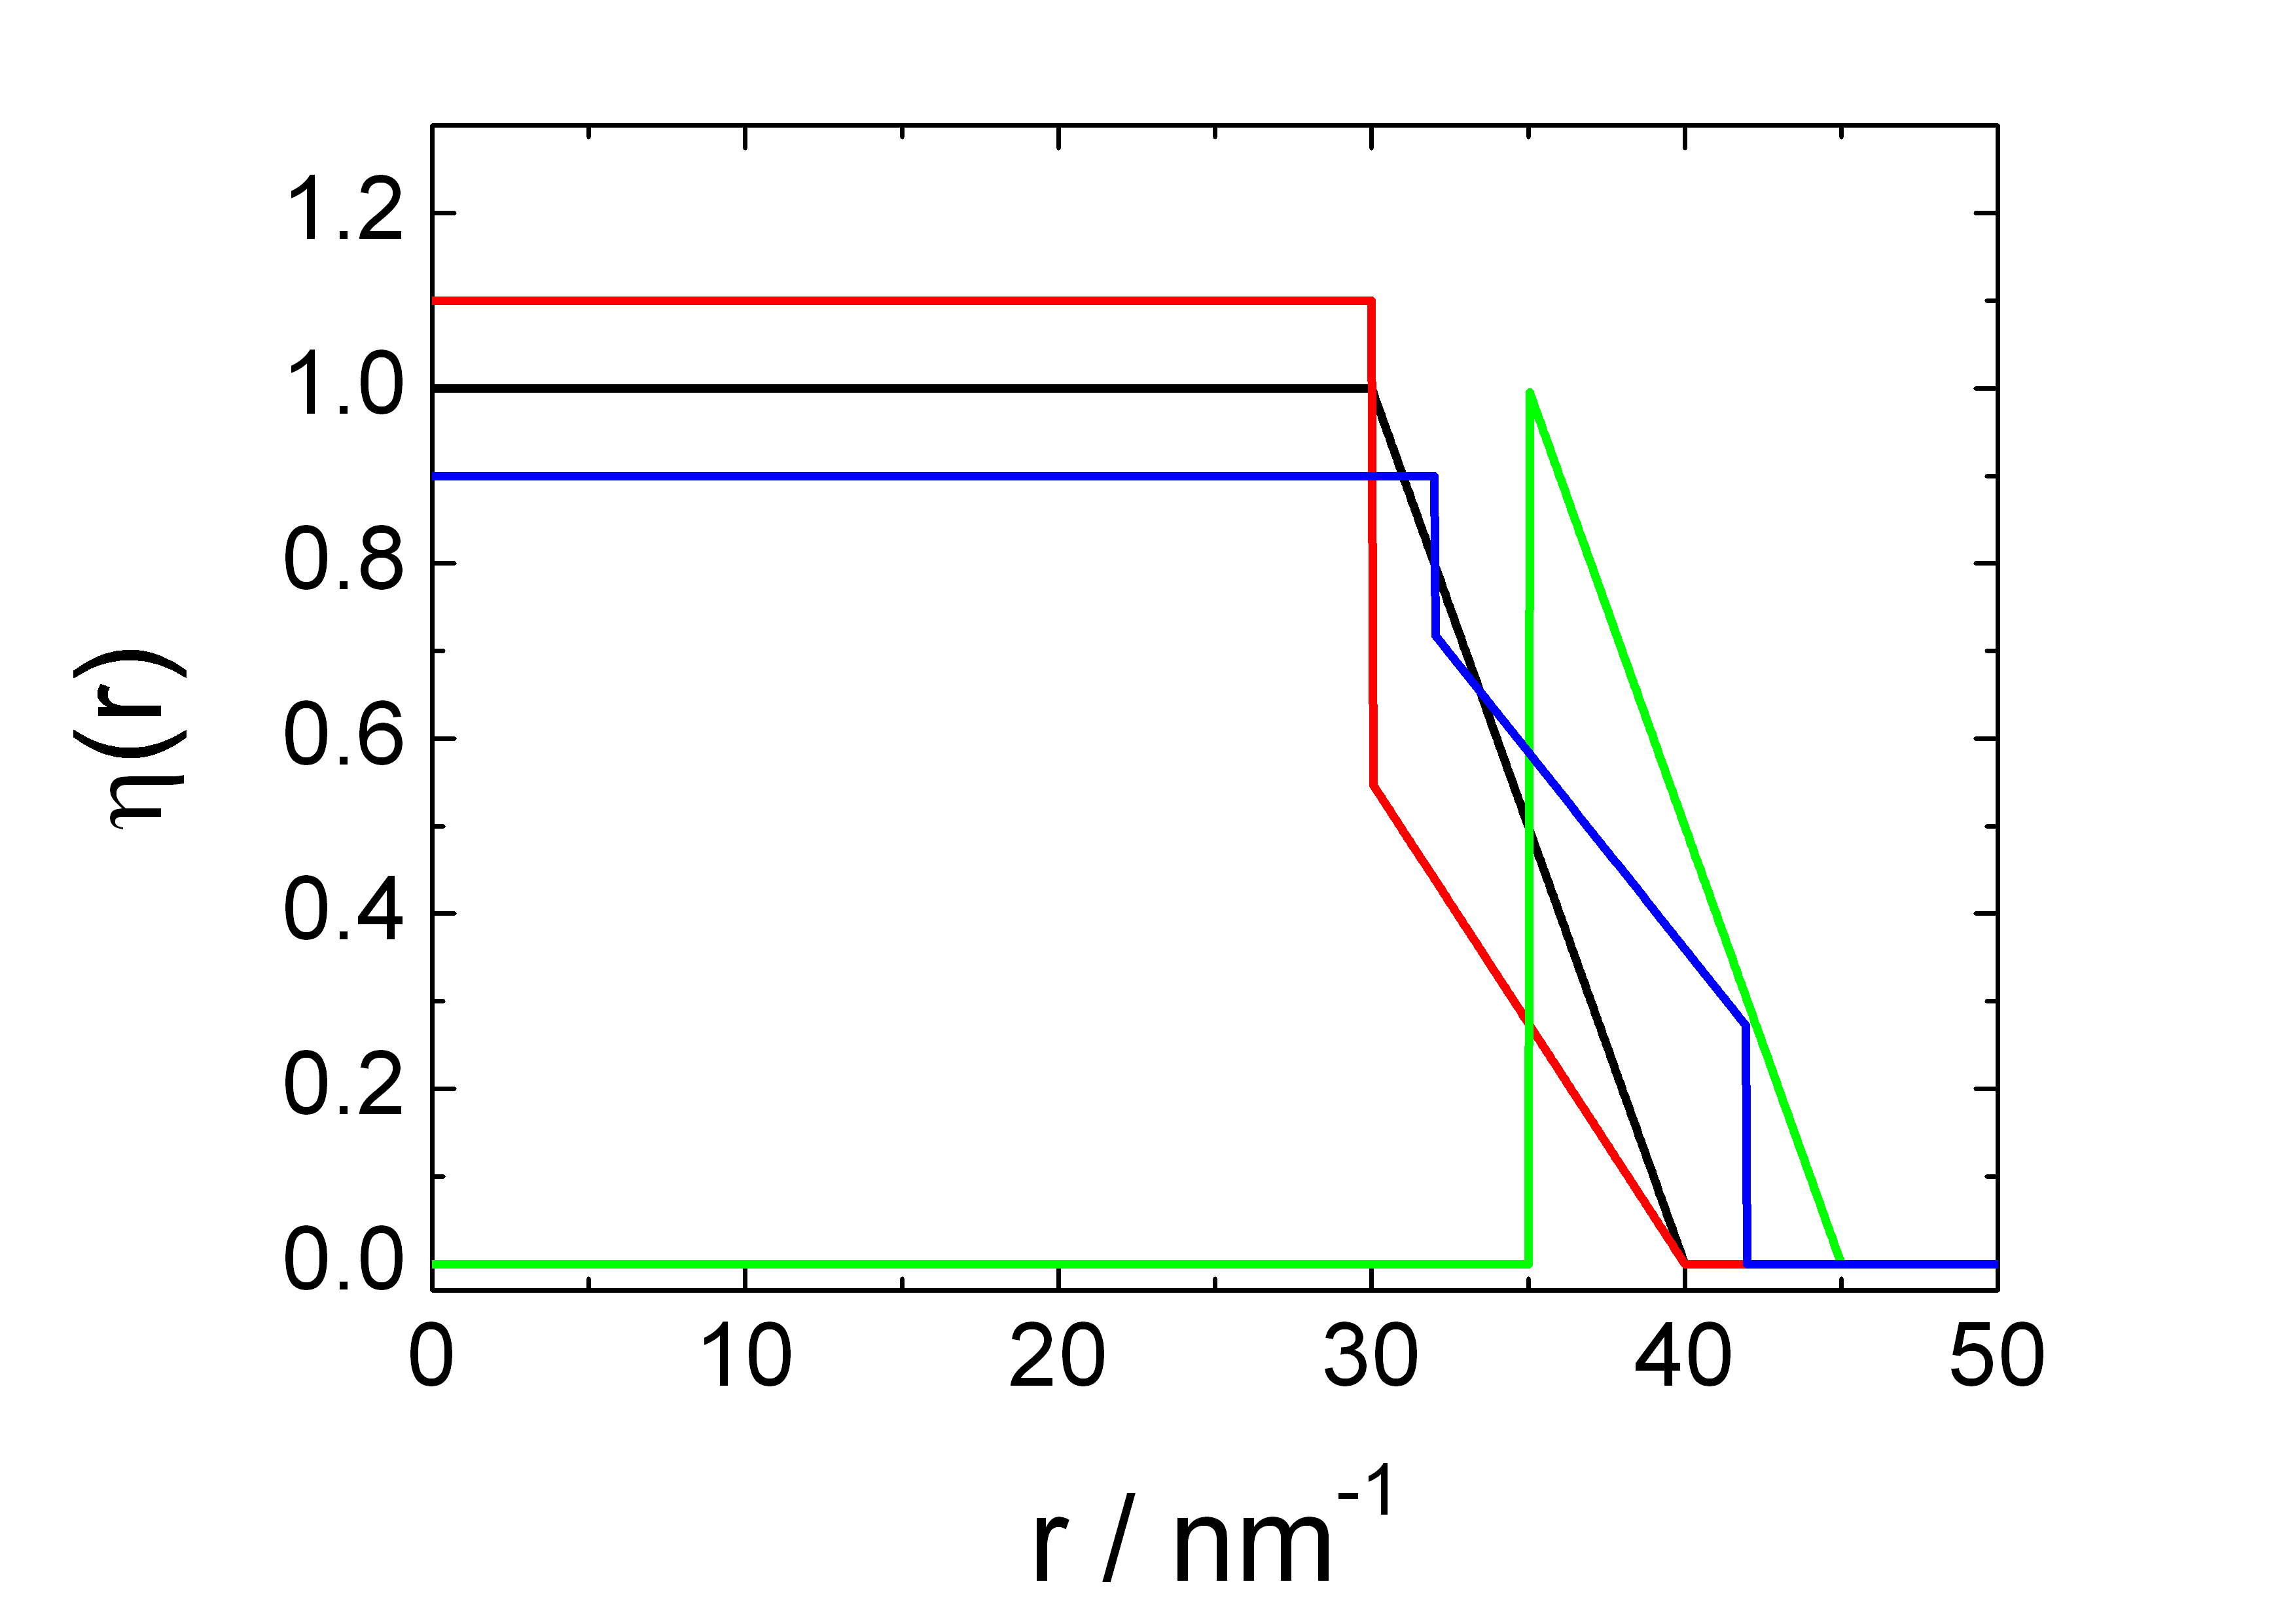
\includegraphics[width=0.48\textwidth,height=0.35\textwidth]{../images/form_factor/FuzzySphere/LinShell_profile.png}}
\hfill
\subfigure[Scattering curves of the radial profiles shown in Fig.\ (a).]{
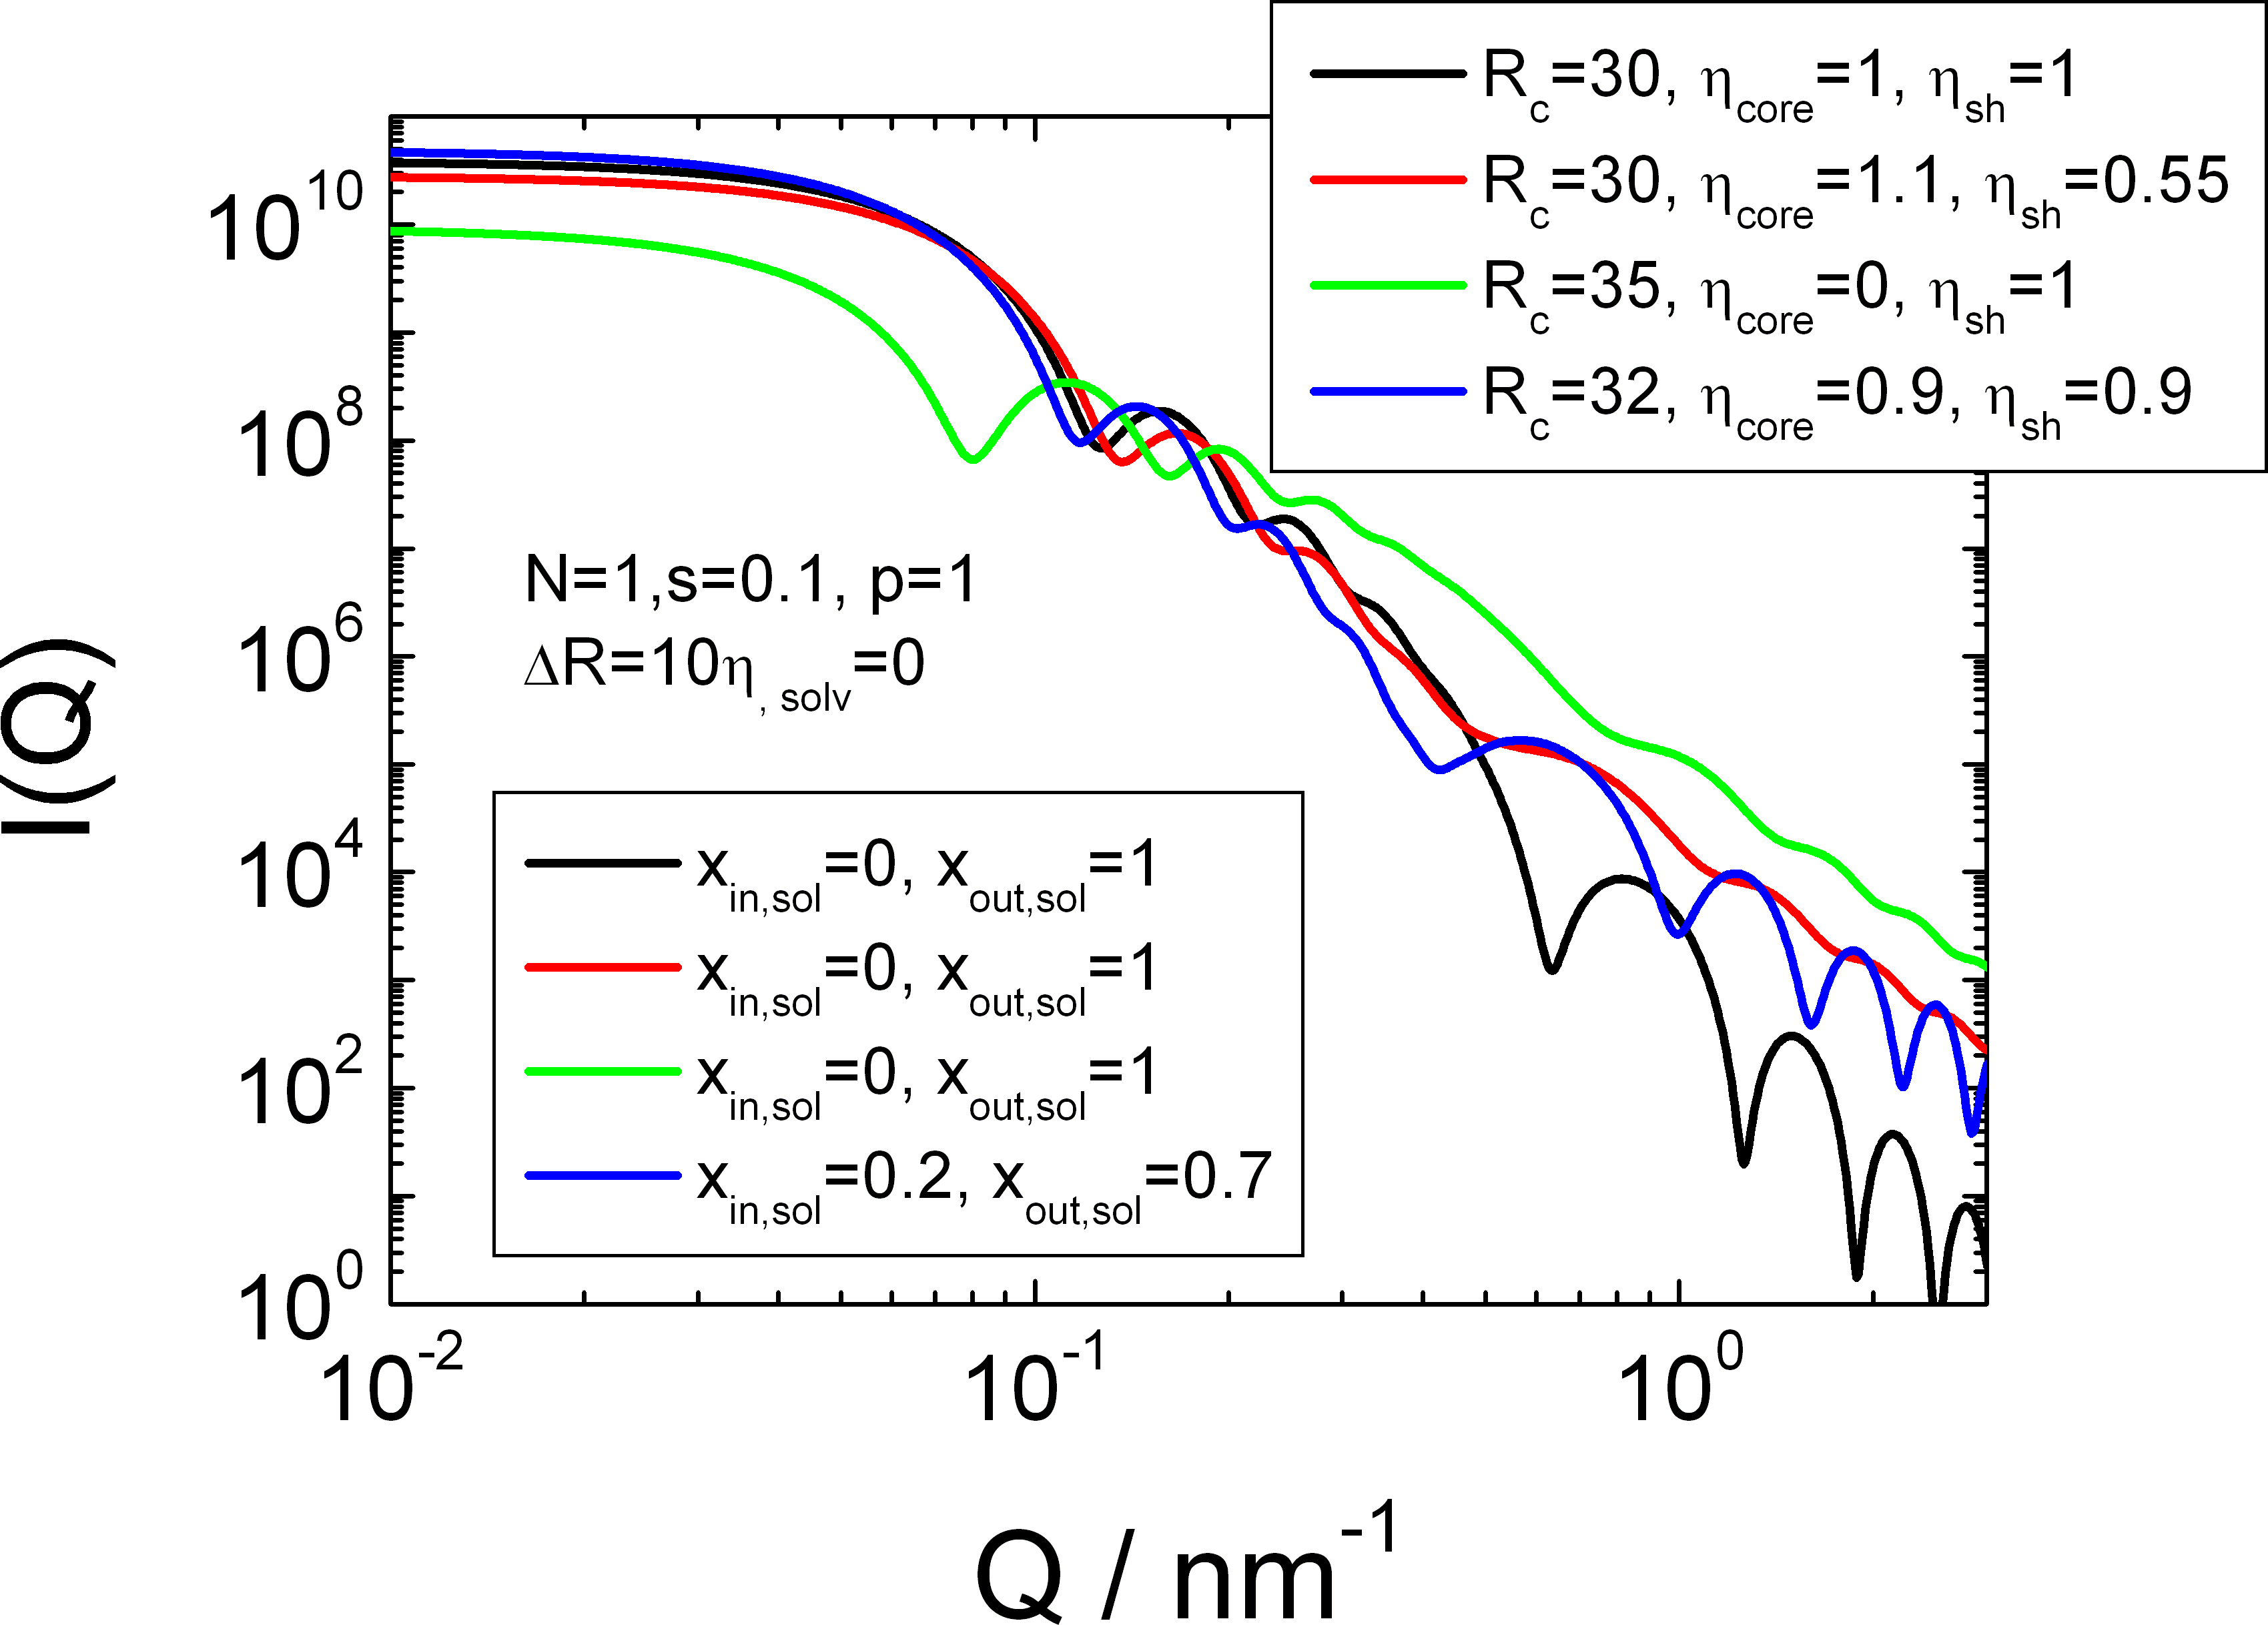
\includegraphics[width=0.48\textwidth,height=0.35\textwidth]{../images/form_factor/FuzzySphere/LinShell_IQ.png}}
\end{center}
\caption{Scattering intensity of a spherical shell with an linear shell profile. The scattering intensity has been calculated
with a lognormal size distribution for the core radius $R_c$.}
\label{fig:I_LinShell1}
\end{figure}
%%%%%%%%%%%%%%%%%%%%%%%%%%%%%%%%%%%%%%%%%%%%%%%%%%%%%%%%%%%%%%%%%%%%%%%%%

\clearpage
\subsection{LinShell2}
\label{sect:LinShell2} ~\\

\begin{figure}[htb]
\begin{center}
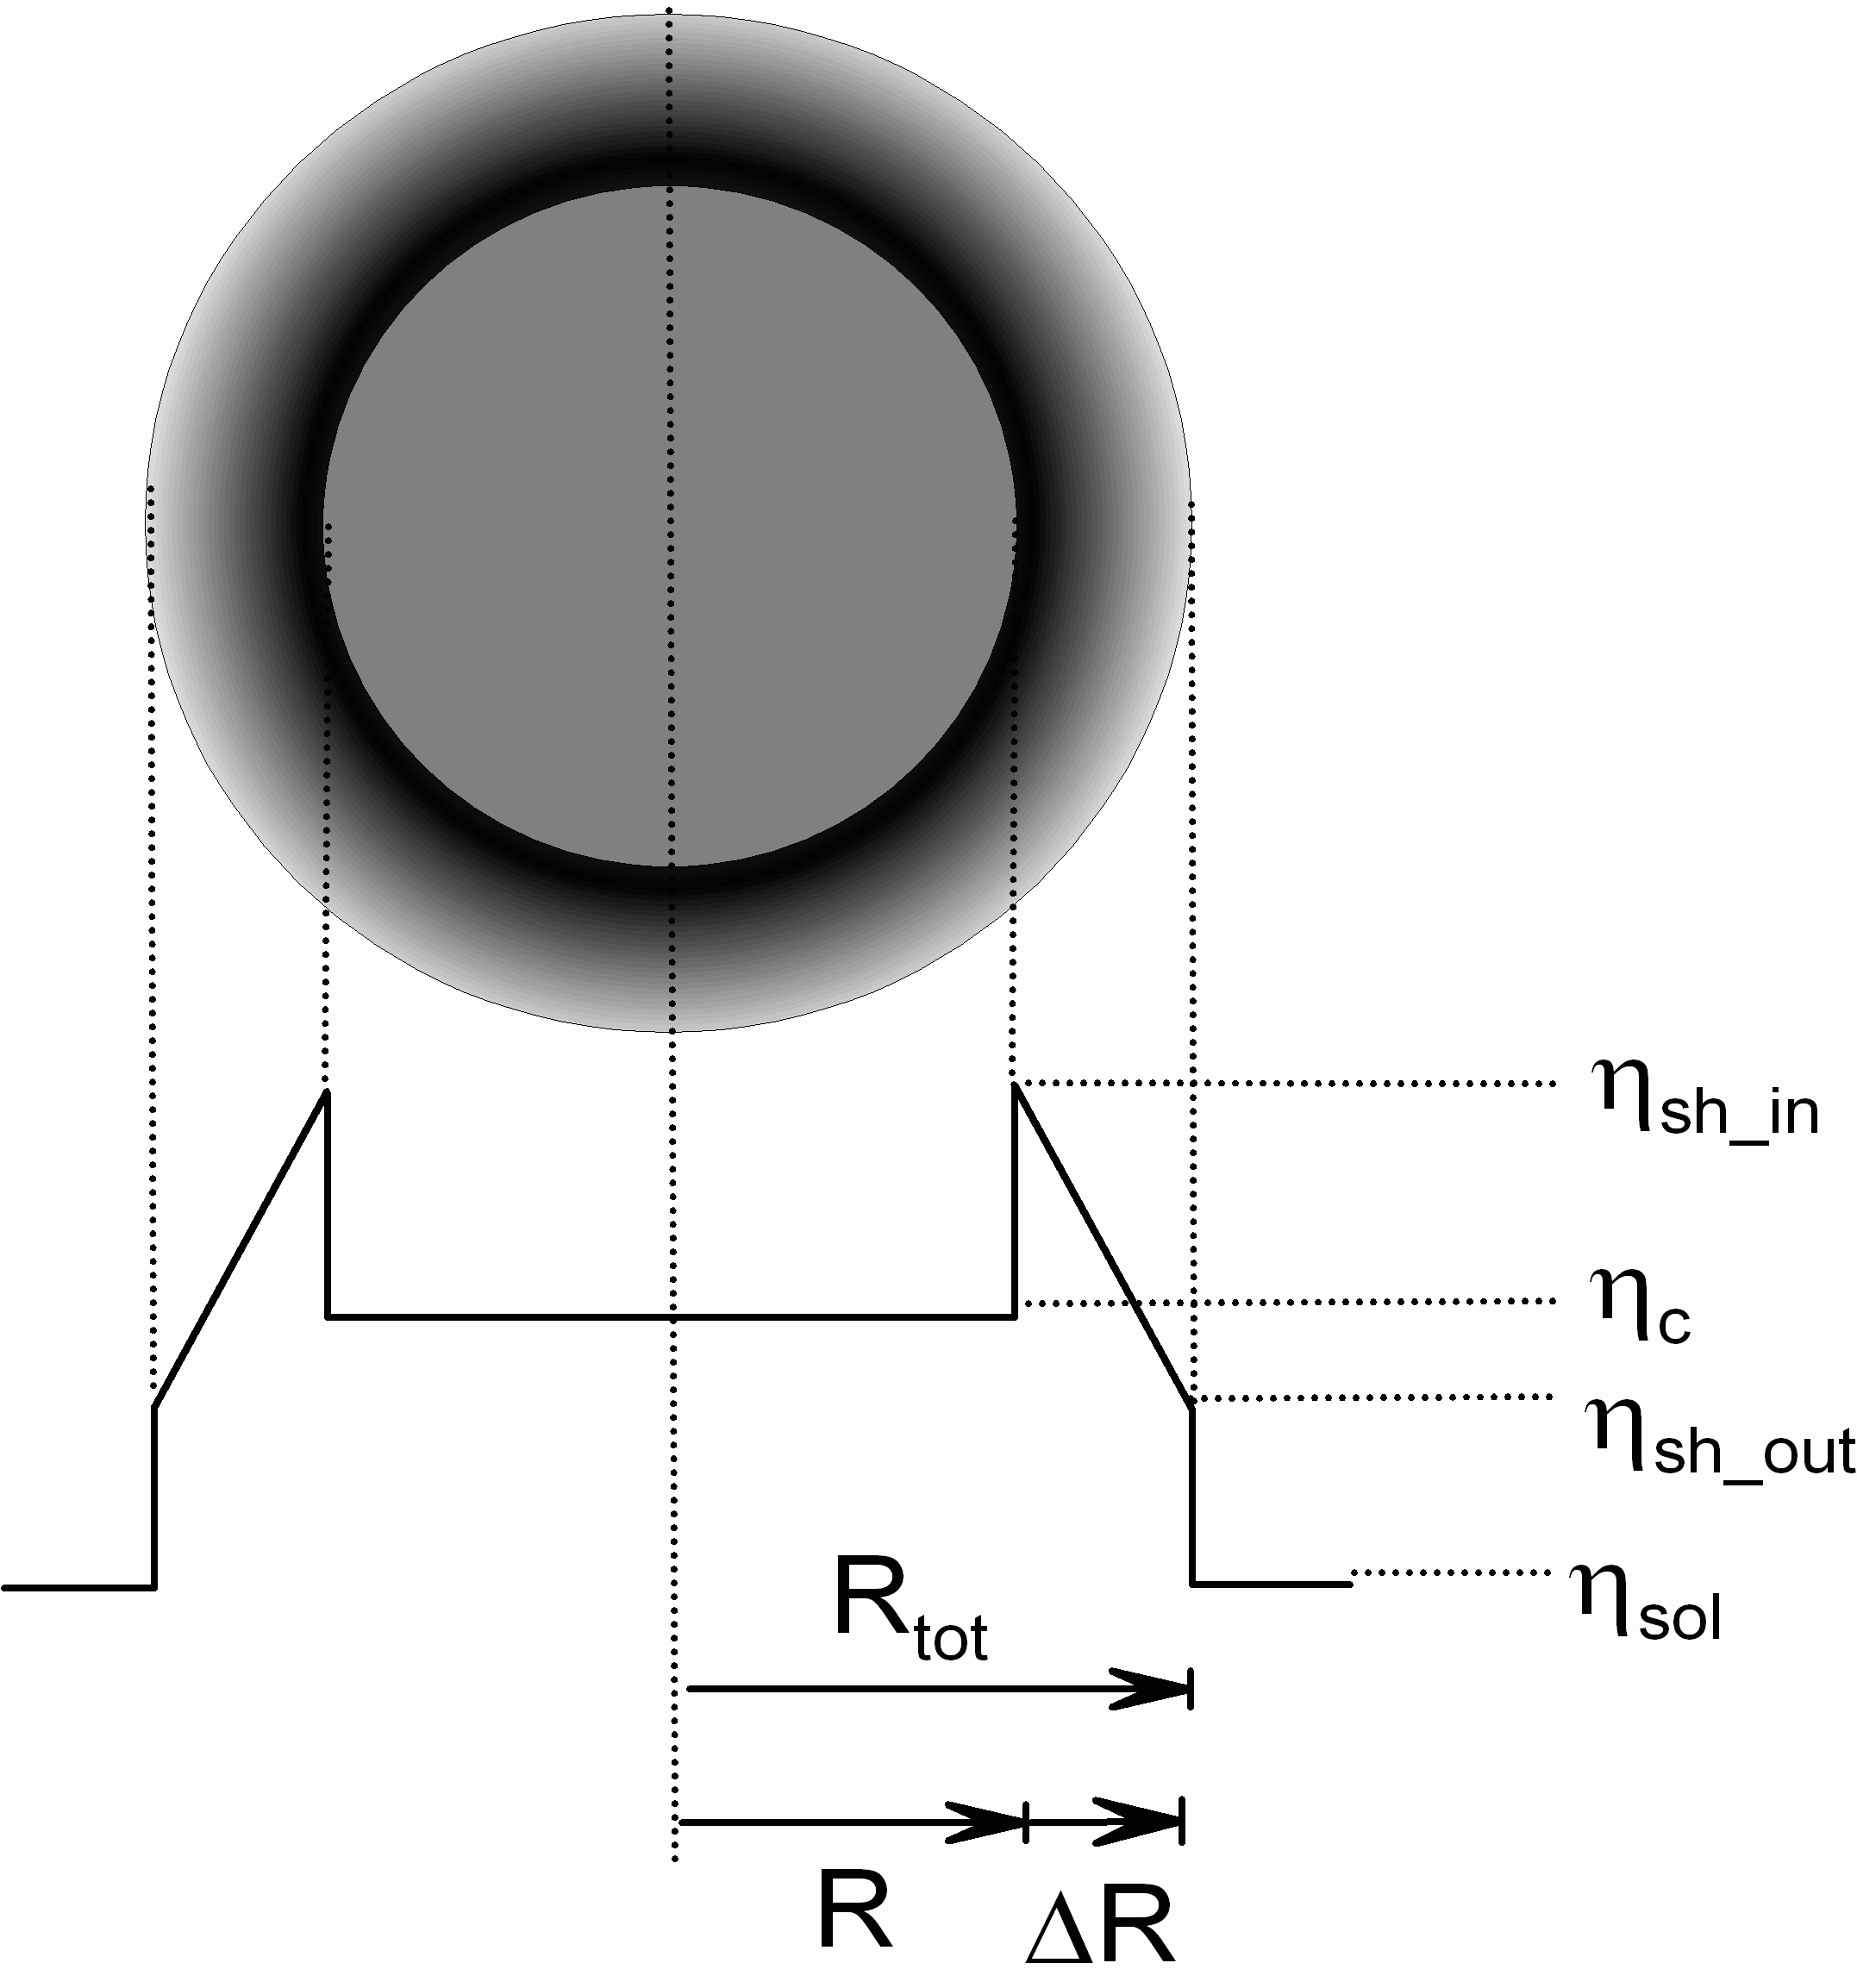
\includegraphics[width=0.5\textwidth,height=0.533\textwidth]{../images/form_factor/spheres/linshell2.png}
\end{center}
\caption{Radial profile for calculating the form factor of a spherical shell with a total
radius $R_\text{tot}$, a shell thickness of $\Delta R$, and a linear varying contrast
profile.} \label{LinShell2Profile}
\end{figure}

Form factor of a spherical shell with a total radius
$R_\text{tot}$ and a shell thickness of $\Delta R$. The definition
are the same than for {\tt LinShell} except that instead of the
core radius $R$ now the total radius $R_\text{tot}$ is used to
parameterize the form factor. The parameter definitions are the
following:
\begin{align}
R&=
\begin{cases}
R_\text{tot}-\Delta R & \mbox{for } R_\text{tot} > \Delta R \\
0 & \mbox{otherwise}
\end{cases}
\end{align}
\begin{align}
\Delta\eta(r)      & =
\begin{cases}
\eta_\text{c} & \text{~for~} r<R \\
m r + b  & \text{~for~} r \in [R,R_\text{tot}] \\
\eta_\text{sol} & \text{~for~} r>R_\text{tot}
\end{cases}
\end{align}
with
\begin{align}
m           & = (\eta_\text{sh\_out}-\eta_\text{sh\_in}) / \Delta R \\
b           & = -m R + \eta_\text{sh\_in}
\end{align}
and
\begin{align}
\eta_\text{sh\_in}  & = (1 - x_\text{in,sol})  \, \eta_\text{sh} + x_\text{in,sol} \,\eta_\text{sol} \\
                    & : \text{scattering length density at $R$} \nonumber \\
\eta_\text{sh\_out} & = (1 - x_\text{out,sol}) \, \eta_\text{sh} + x_\text{out,sol}\,\eta_\text{sol} \\
                    & : \text{scattering length density at $R_\text{tot}=R+\Delta R$} \nonumber \\
\eta_\text{sh}      & : \text{scattering length density of pure shell material} \nonumber \\
\eta_\text{c}       & : \text{scattering length density of core} \nonumber \\
x_\text{in,sol}     & : \text{amount of solvent at $R$} \nonumber \\
x_\text{out,sol}    & : \text{amount of solvent at $R_\text{tot}=R+\Delta R$} \nonumber
\end{align}

\begin{align}
F_\text{sph}(A,x) & = \frac{4}{3}\pi x^3 \,\, 3\frac{\sin(A)-A\cos(A)}{A^3} \\[5mm]
F_\text{shlin}(A,x) & = 4\pi x^4 \frac{2\cos(A)+2A\sin(A)-A^2\cos(A)}{A^4} \\[5mm]
I_\text{LinShell2}    & = \big[ \,\, (\eta_\text{c}-\eta_\text{sol}-b)F_\text{sph}(QR,R) \nonumber \\
             & \hspace{6mm} - mF_\text{shlin}(QR,R) \\
             & \hspace{6mm} + mF_\text{shlin}\left(QR_\text{tot},R_\text{tot}\right) \nonumber \\
             & \hspace{6mm} + bF_\text{sph}\left(QR_\text{tot},R_\text{tot}\right) \big]^2 \nonumber
\end{align}

\vspace{5mm}

\hspace{1pt}\\
\underline{Input Parameters for model \texttt{LinShell2} and \texttt{radial profile of LinShell2}:}\\
\begin{description}
\item[\texttt{Rtot}] total overall radius $R_\text{tot}$
\item[\texttt{dR}] thickness of the shell $\Delta R$
\item[\texttt{eta\_c}] scattering length density $\eta_\text{c}$
\item[\texttt{eta\_sh}] scattering length density of non-swollen shell $\eta_\text{sh}$
\item[\texttt{x\_in}] amount of solvent $x_\text{in,sol}$ on core-shell interface at $R$ $(x_\text{in,sol} \in [0;1])$
\item[\texttt{x\_out}] amount of solvent $x_\text{out,sol}$ on shell-solvent interface at $R+\Delta R$ $(x_\text{out,sol} \in [0;1])$.
\item[\texttt{eta\_s}] scattering length density of solvent $\eta_\text{sol}$
\end{description}


\noindent\underline{Note:}
\begin{itemize}
\item $x_\text{in,sol}$ and $x_\text{out,sol}$ are only physical for values between 0 and 1.
\end{itemize}

%%%%%%%%%%%%%%%%%%%%%%%%%%%%%%%%%%%%%%%%%%%%%%%%%%%%%%%%%%%%%%%%%%%%%%%%%

\clearpage
\subsection{ExpShell}
\label{sect:ExpShell} ~\\

\begin{figure}[htb]
\begin{center}
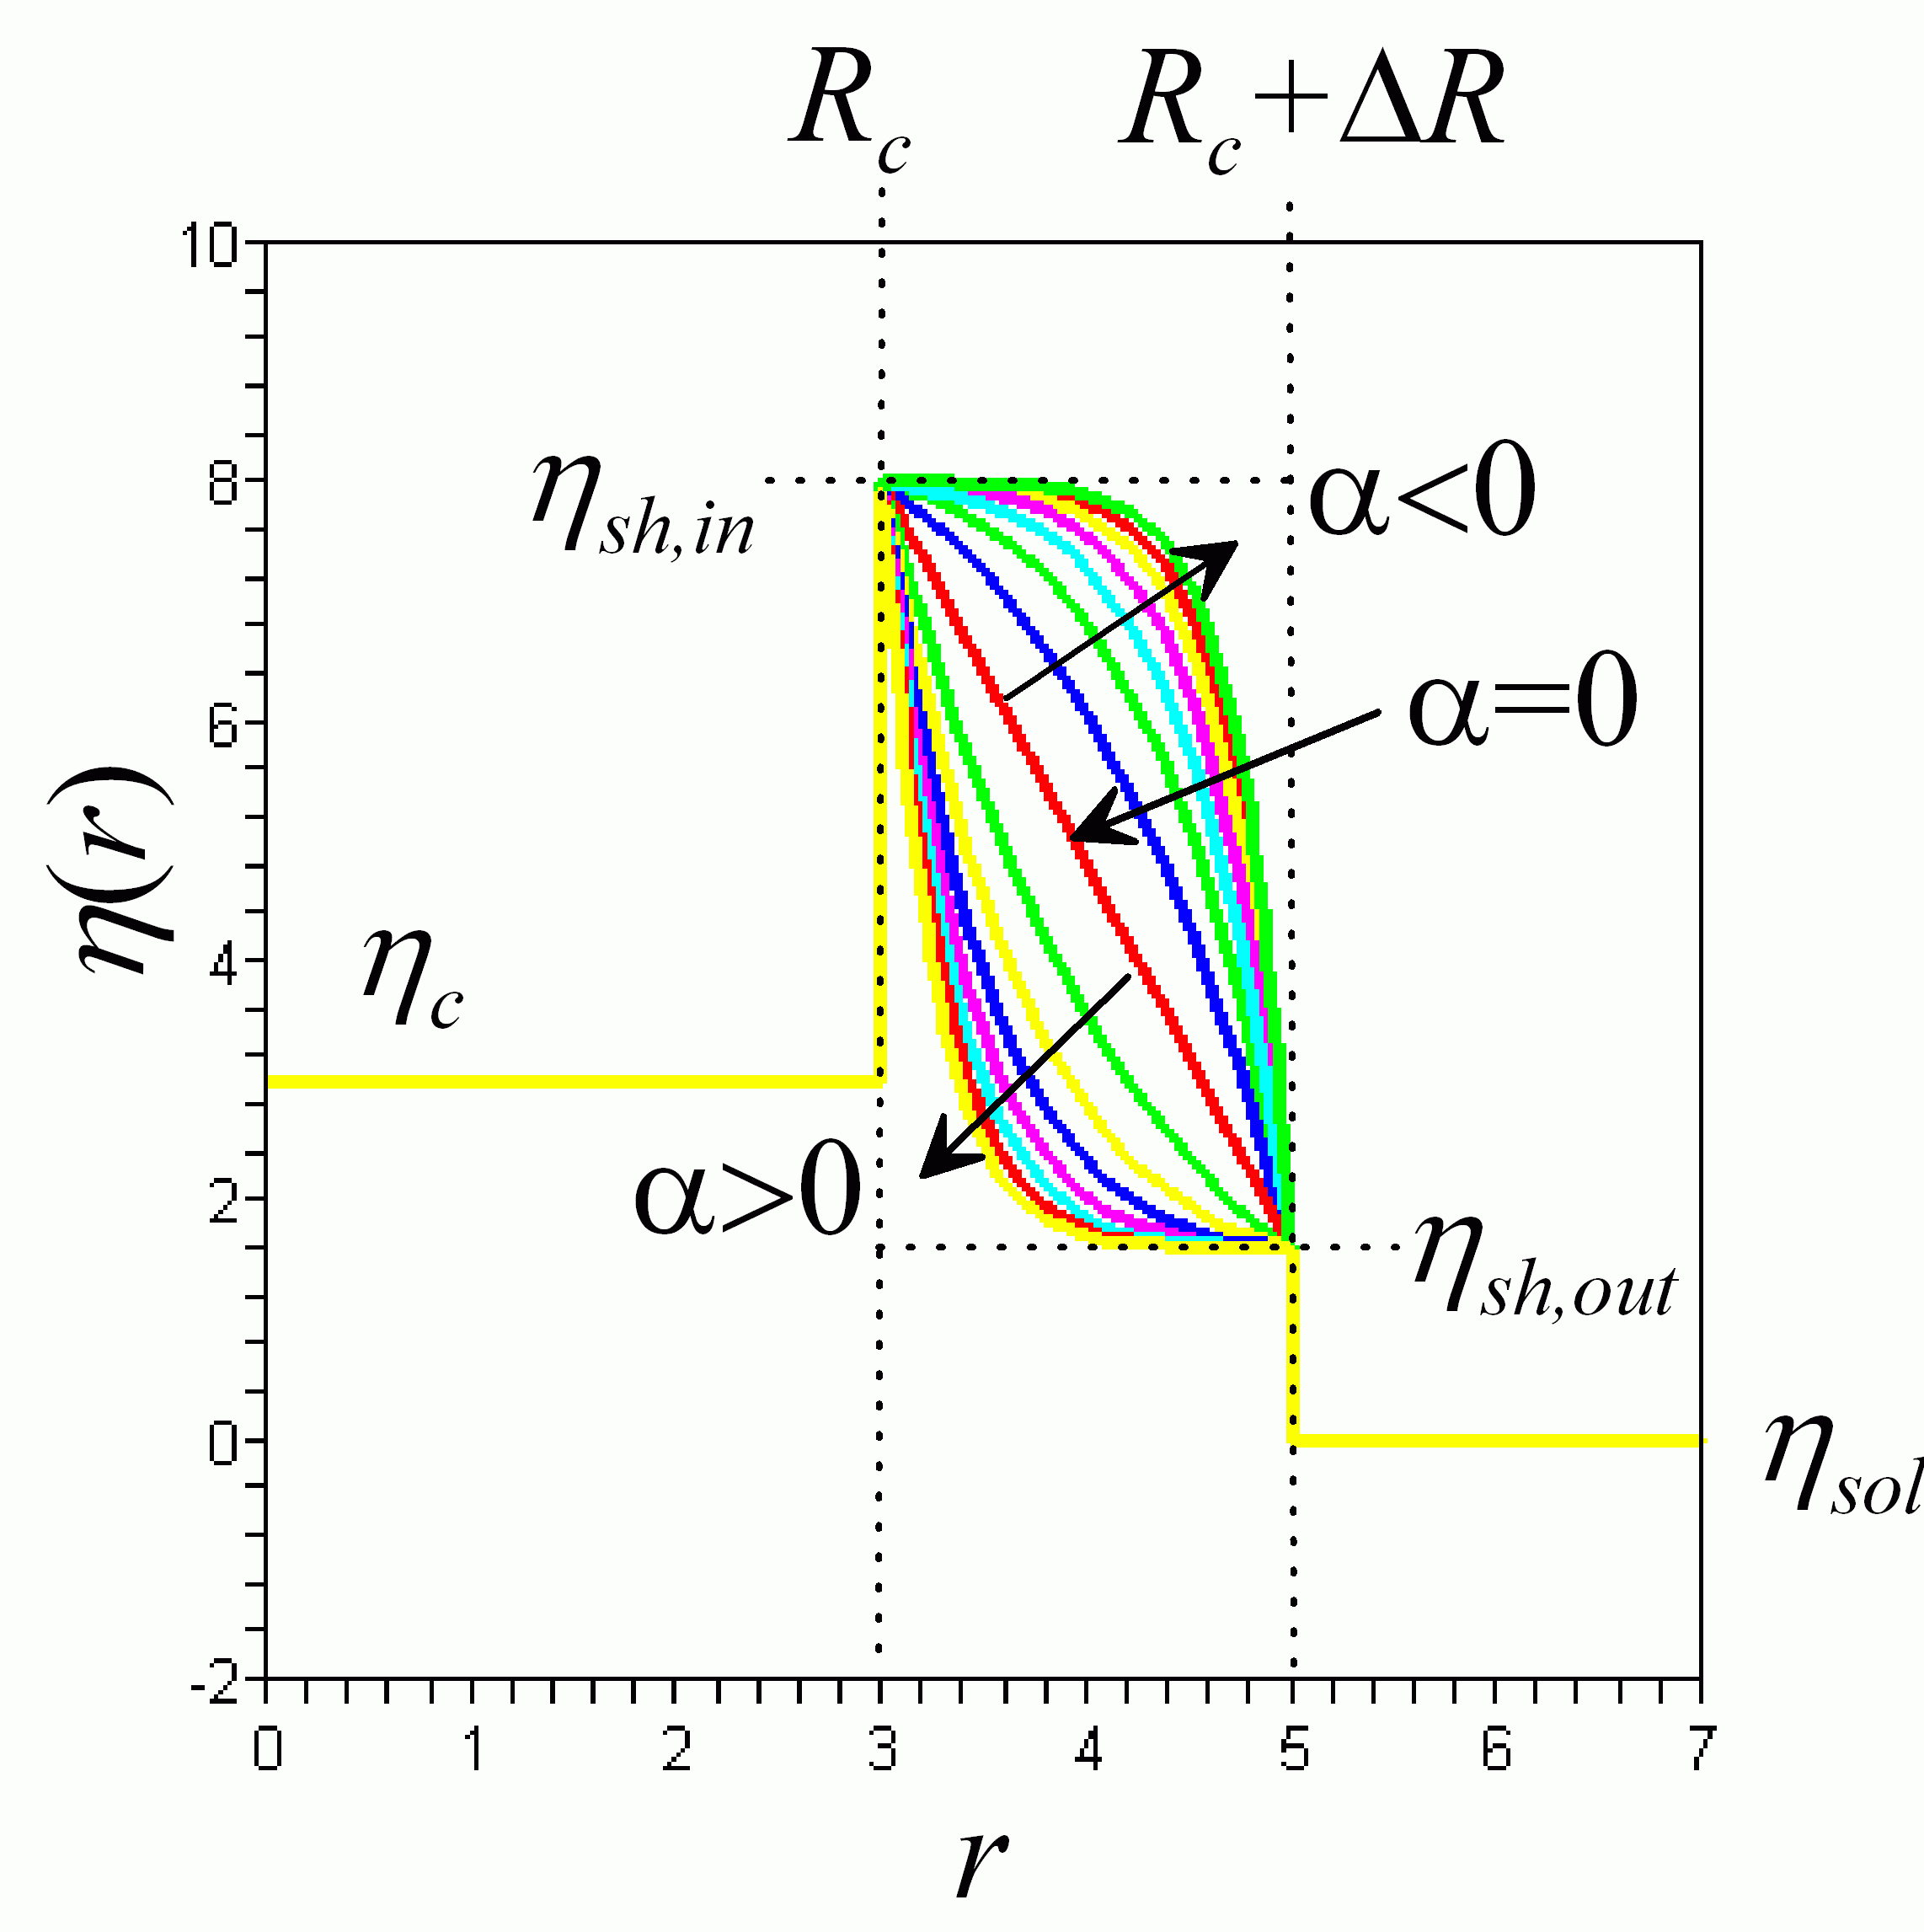
\includegraphics[width=0.55\textwidth,height=0.5\textwidth]{../images/form_factor/spheres/ExpShell.png}
\end{center}
\caption{Radial profile for calculating the form factor of a spherical shell with a core radius
$R_c$ and a shell thickness of $\Delta R$ and a exponentially varying contrast
profile. The profile shape can be varied by the parameter $\alpha$ describing the penetration of the solvent into the shell.
A value of $\alpha=0$ means linear profile and is equivalent to {\tt LinShell}
and {\tt LinShell2}. For $\alpha>0$ the solvent penetrates further into the shell
and for $\alpha<0$ less.} \label{ExpShellProfile}
\end{figure}

\noindent
\begin{align}
\eta_\text{ExpShell}(r,R_c,\Delta R,\alpha,\phi_\text{in},\phi_\text{out}) &=
\begin{cases}
\eta_c              & r \leq R_c  \\
\eta_\text{exp}(\frac {r-R_c}{\Delta R})   & R_c < r< R_c+\Delta R \\
\eta_\text{sol}     & r> R_c+\Delta R
\end{cases}
\end{align}
\begin{align}
\eta_\text{exp} (x) &=
\begin{cases}
\eta_\text{sh,in}  +
\left[\eta_\text{sh,out}-\eta_\text{sh,in}\right] x \exp\left( \left[ 1-x \right] \alpha\right)
 & \alpha<0 \\[2mm]
\left[\eta_\text{sh,in}-\eta_\text{sh,out}\right] \left[1-x\right] \exp\left(-{x\alpha}\right) +
 \eta_\text{sh,out}& \alpha \geq 0
\end{cases} \\[2mm]
\eta_\text{sh,in} & = \left[ \phi_\text{in}\,\eta_\text{sol}+ \left( 1-\phi_\text{in} \right)
 \eta_\text{sh} \right] \\
\eta_\text{sh,out} & = \left[ \phi_\text{out}\,\eta_\text{sol}+ \left( 1-\phi_\text{out} \right) \eta_\text{sh} \right]
\end{align}

The scattering intensity for the radial symmetric scattering length density profile $\eta_\text{ExpShell}(r)$
can be calculated analytical. The integral needed to be solved for that is
\begin{equation}
I_\text{ExpShell}(Q) = \int_0^\infty 4\pi r^2 \frac{\sin Qr}{Qr}\, \eta_\text{ExpShell}(r)\, dr
\end{equation}

\begin{align}
R_c &=\text{core radius} \nonumber\\
\Delta R &=\text{shell thickness} \nonumber\\
\eta_\text{sh,in}  & = (1 - \phi_\text{in,sol})  \, \eta_\text{sh} + \phi_\text{in,sol} \,\eta_\text{sol} \\
                    & : \text{scattering length density at $R_c$} \nonumber \\
\eta_\text{sh,out}     & = (1 - \phi_\text{out,sol}) \, \eta_\text{sh} + \phi_\text{out,sol}\,\eta_\text{sol} \\
                        & : \text{scattering length density at $R_c+\Delta R$} \nonumber \\
\eta_\text{sh}      & : \text{scattering length density of pure shell material} \nonumber \\
\eta_\text{c}       & : \text{scattering length density of core} \nonumber \\
\phi_\text{in}     & : \text{amount of solvent  at $R_c$} \nonumber \\
\phi_\text{out}    & : \text{amount of solvent at $R_c+\Delta R$} \nonumber \\
\alpha             & : \text{parameter for exponential diffuse profile of the shell} \\
\nonumber
\end{align}


\vspace{5mm}

\hspace{1pt}\\
\underline{Input Parameters for model \texttt{ExpShell}:}\\
\begin{description}
\item[\texttt{R\_core}] radius of core  $R_c$
\item[\texttt{DR}] thickness of the shell $\Delta R$
\item[\texttt{eta\_core}] scattering length density $\eta_\text{c}$
\item[\texttt{eta\_shell}] scattering length density of non-swollen shell $\eta_\text{sh}$
\item[\texttt{x\_in\_sol}] amount of solvent $\phi_\text{in}$ on core-shell interface at $r=R$
\item[\texttt{x\_out\_sol}] amount of solvent $\phi_\text{out}$ on shell-solvent interface at $r=R+\Delta R$
\item[\texttt{alpha}]  a parameter ($\alpha$) which describes the penetration profile of the solvent into the shell.
A value of $\alpha=0$ means linear profile and is equivalent to {\tt LinShell} and {\tt LinShell2}. For $\alpha>0$
the solvent penetrates further into the shell and for $\alpha<0$ less.
\item[\texttt{eta\_solvent}] scattering length density of solvent $\eta_\text{sol}$
\end{description}

\noindent\underline{Note:}
\begin{itemize}
\item $\phi_\text{in}$ and $\phi_\text{out}$ are only physical for values between 0 and 1.
\end{itemize}

\begin{figure}[htb]
\begin{center}
\subfigure[Some radial profiles of spheres with a exponential interfaces
which have been used to calculate the scattering curve in Fig.\ (b).
]{
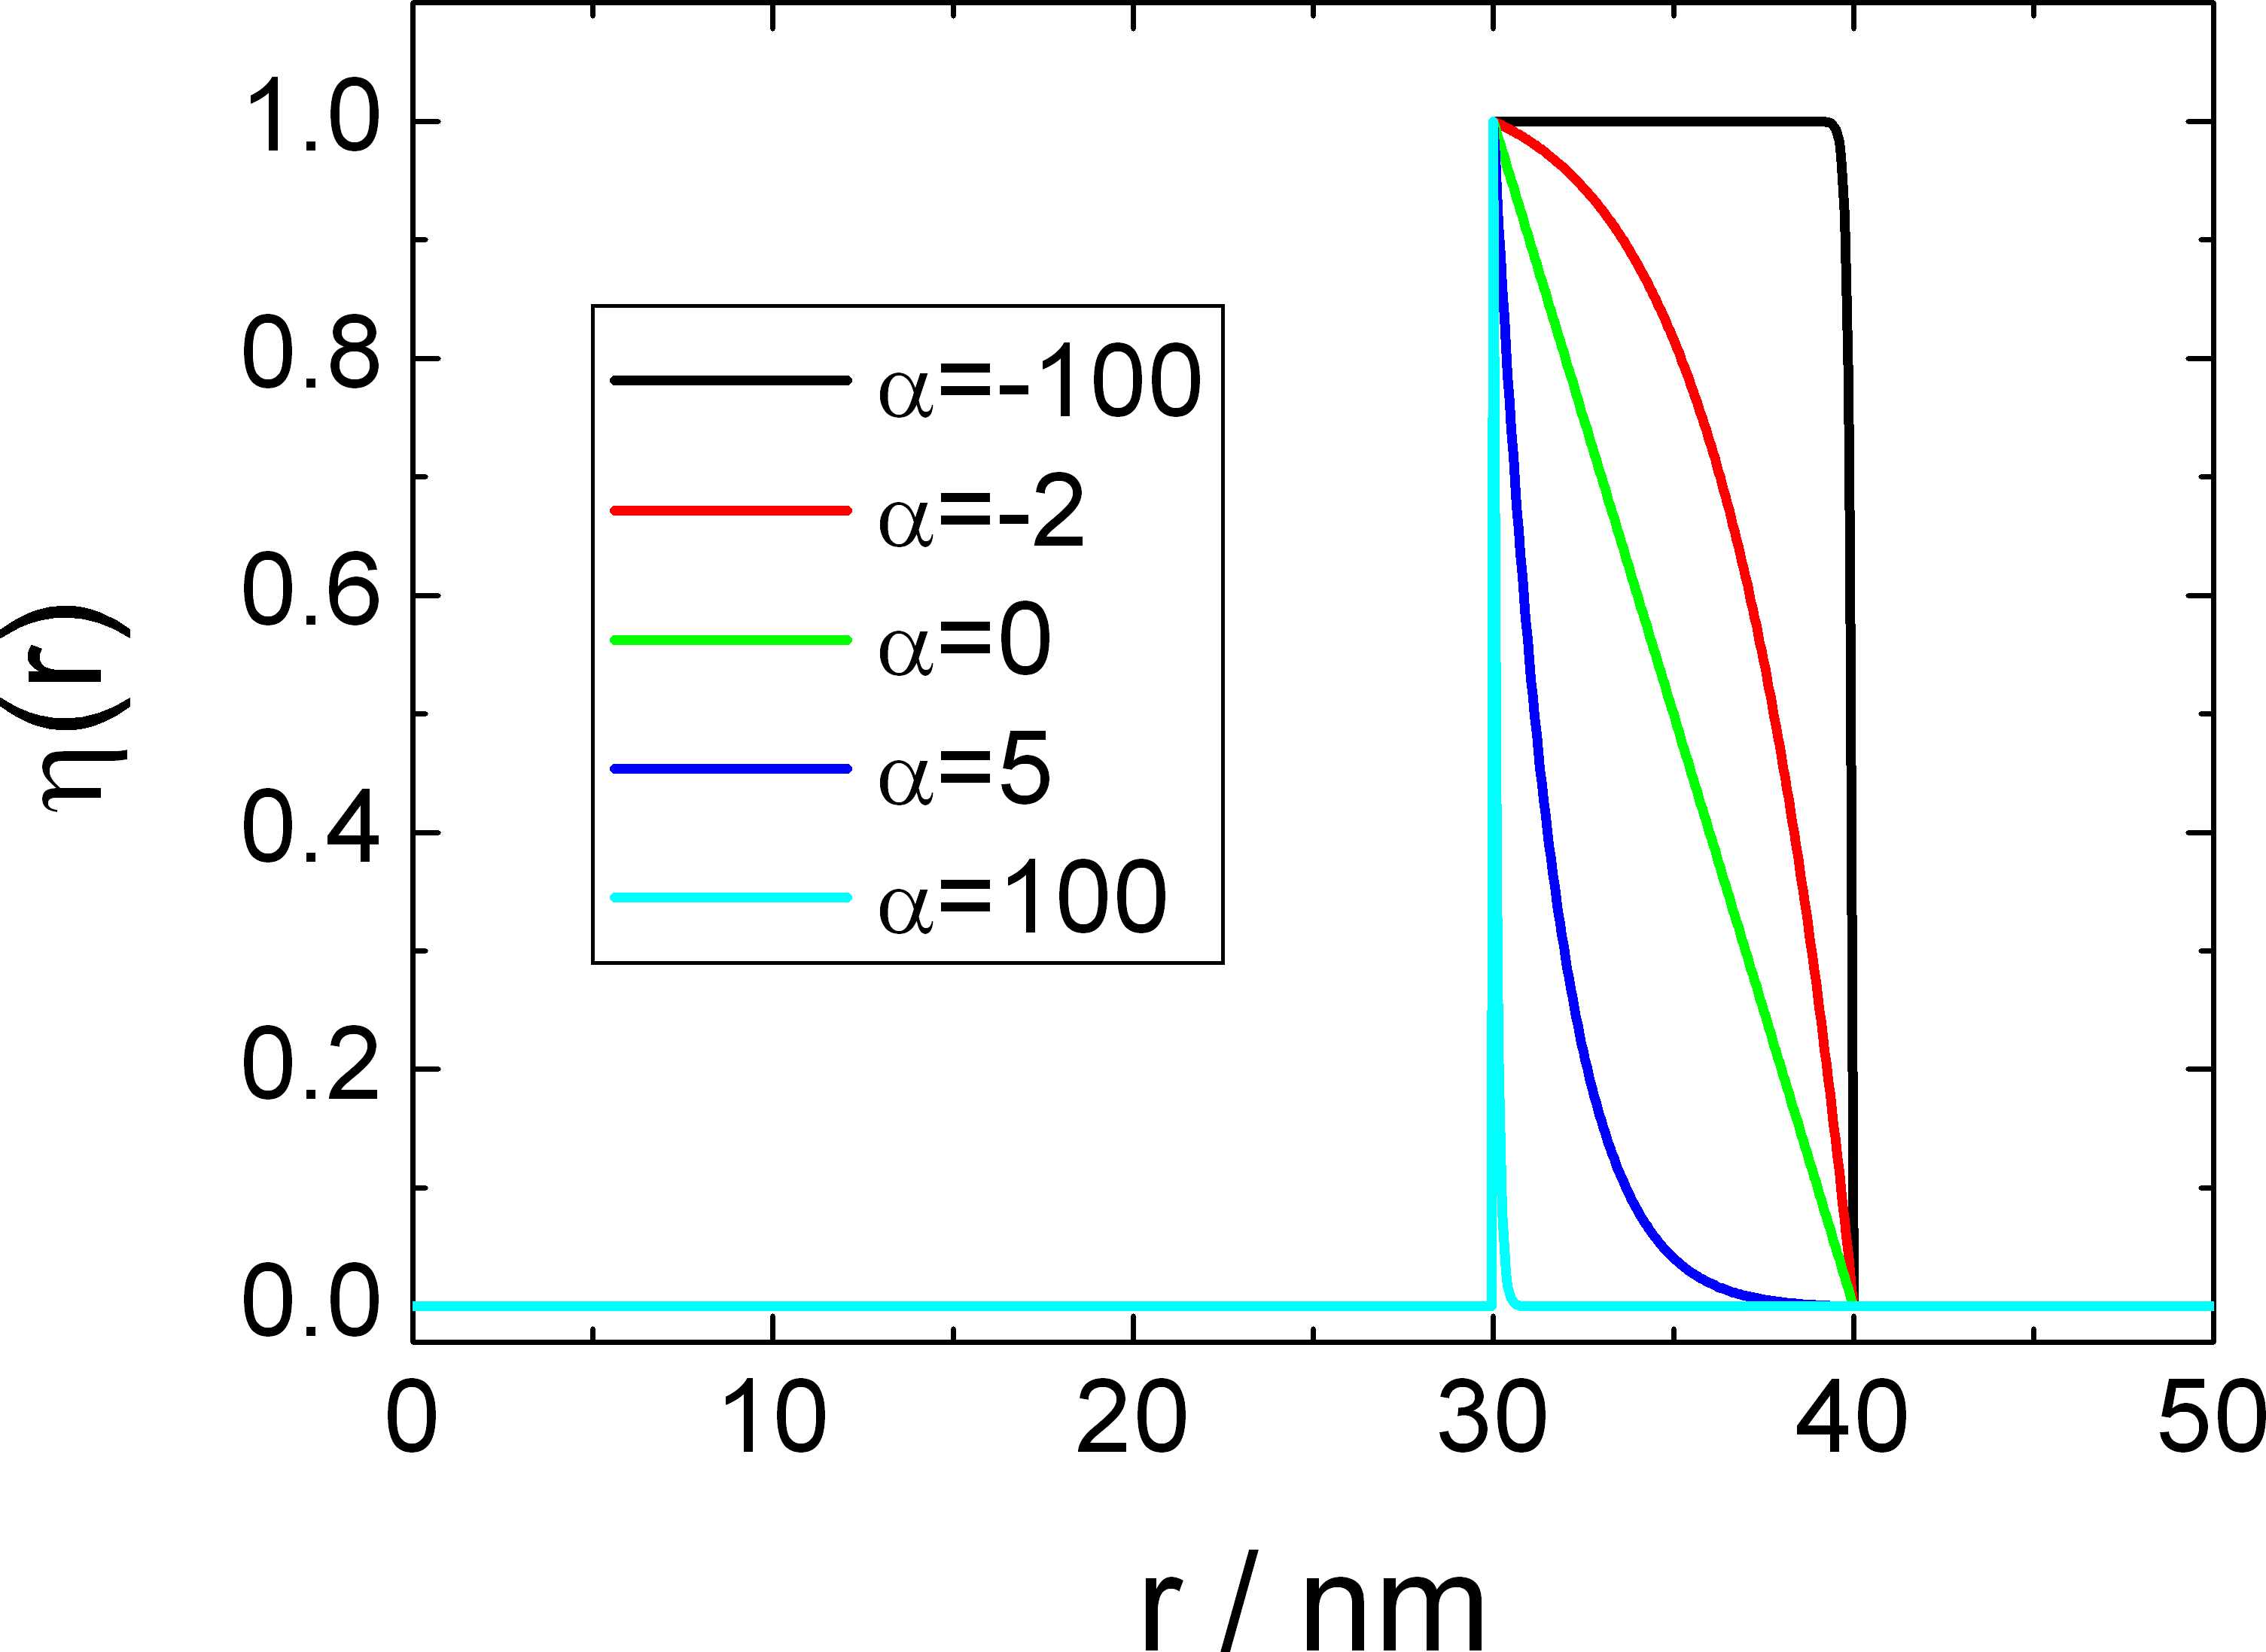
\includegraphics[width=0.48\textwidth,height=0.35\textwidth]{../images/form_factor/FuzzySphere/ExpShell_profile.png}}
\hfill
\subfigure[Scattering curves of the radial profiles shown in Fig.\ (a).]{
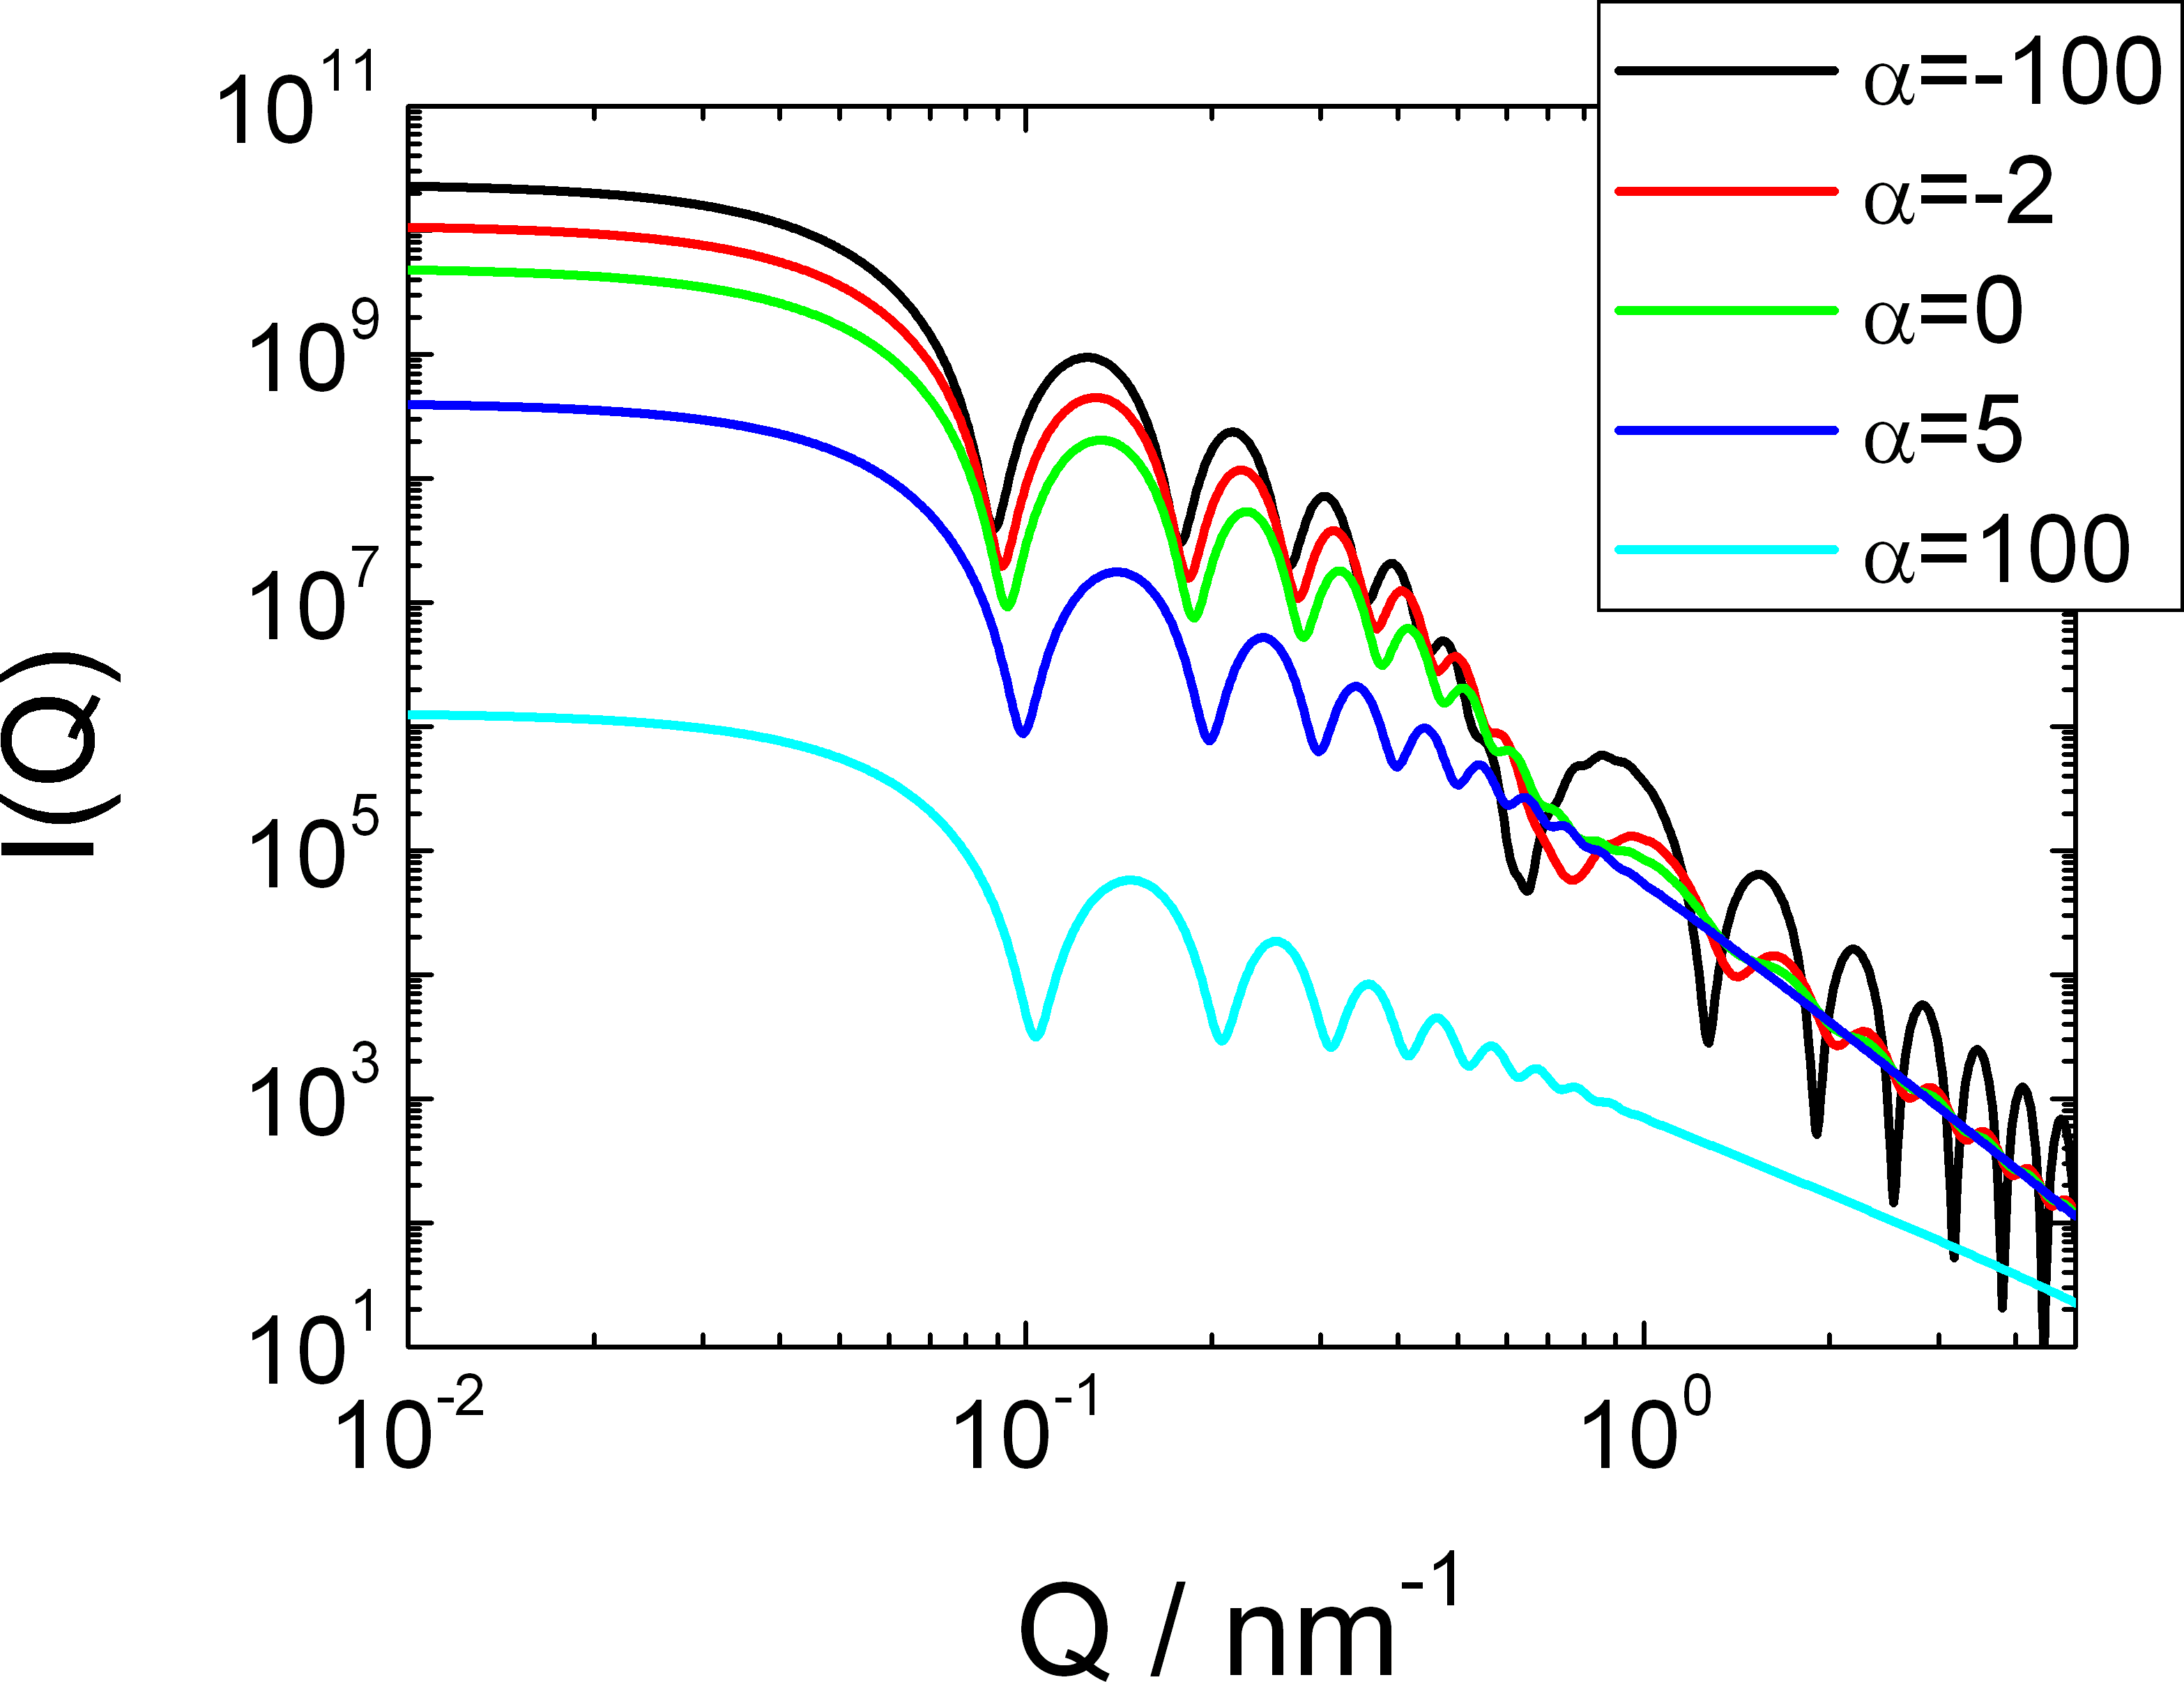
\includegraphics[width=0.48\textwidth,height=0.35\textwidth]{../images/form_factor/FuzzySphere/ExpShell_IQ.png}}
\end{center}
\caption{Scattering intensity of a spherical shell with an exponential shell profile. The scattering intensity has been calculated
with a lognormal $[\mathrm{LogNorm}(N\!=\!1,\sigma\!=\!0.05,p\!=\!1,R\!=\!30)]$ size distribution for the core radius $R_c$.
The scattering length density of the core $\eta_\text{c}$ and the solvent $\eta_\text{sol}$ are set to 0, $\eta_\text{sh}=1$,
$\phi_\text{in}=0$,  $\phi_\text{out}=1$, and $\Delta R =10$.}
\label{fig:ExpShellExample}
\end{figure}

%%%%%%%%%%%%%%%%%%%%%%%%%%%%%%%%%%%%%%%%%%%%%%%%%%%%%%%%%%%%%%%%%%%%%%%%%

\clearpage
\subsection{BoucherSphere, radial profile for a sphere resulting in a Porod law both below and above $q^{-4}$}
\label{sect:BoucherSphere} ~\\

\begin{figure}[htb]
\begin{center}
\subfigure[Some radial profiles with $\eta_0=\Delta\eta$ for several values of $\alpha$.
]{
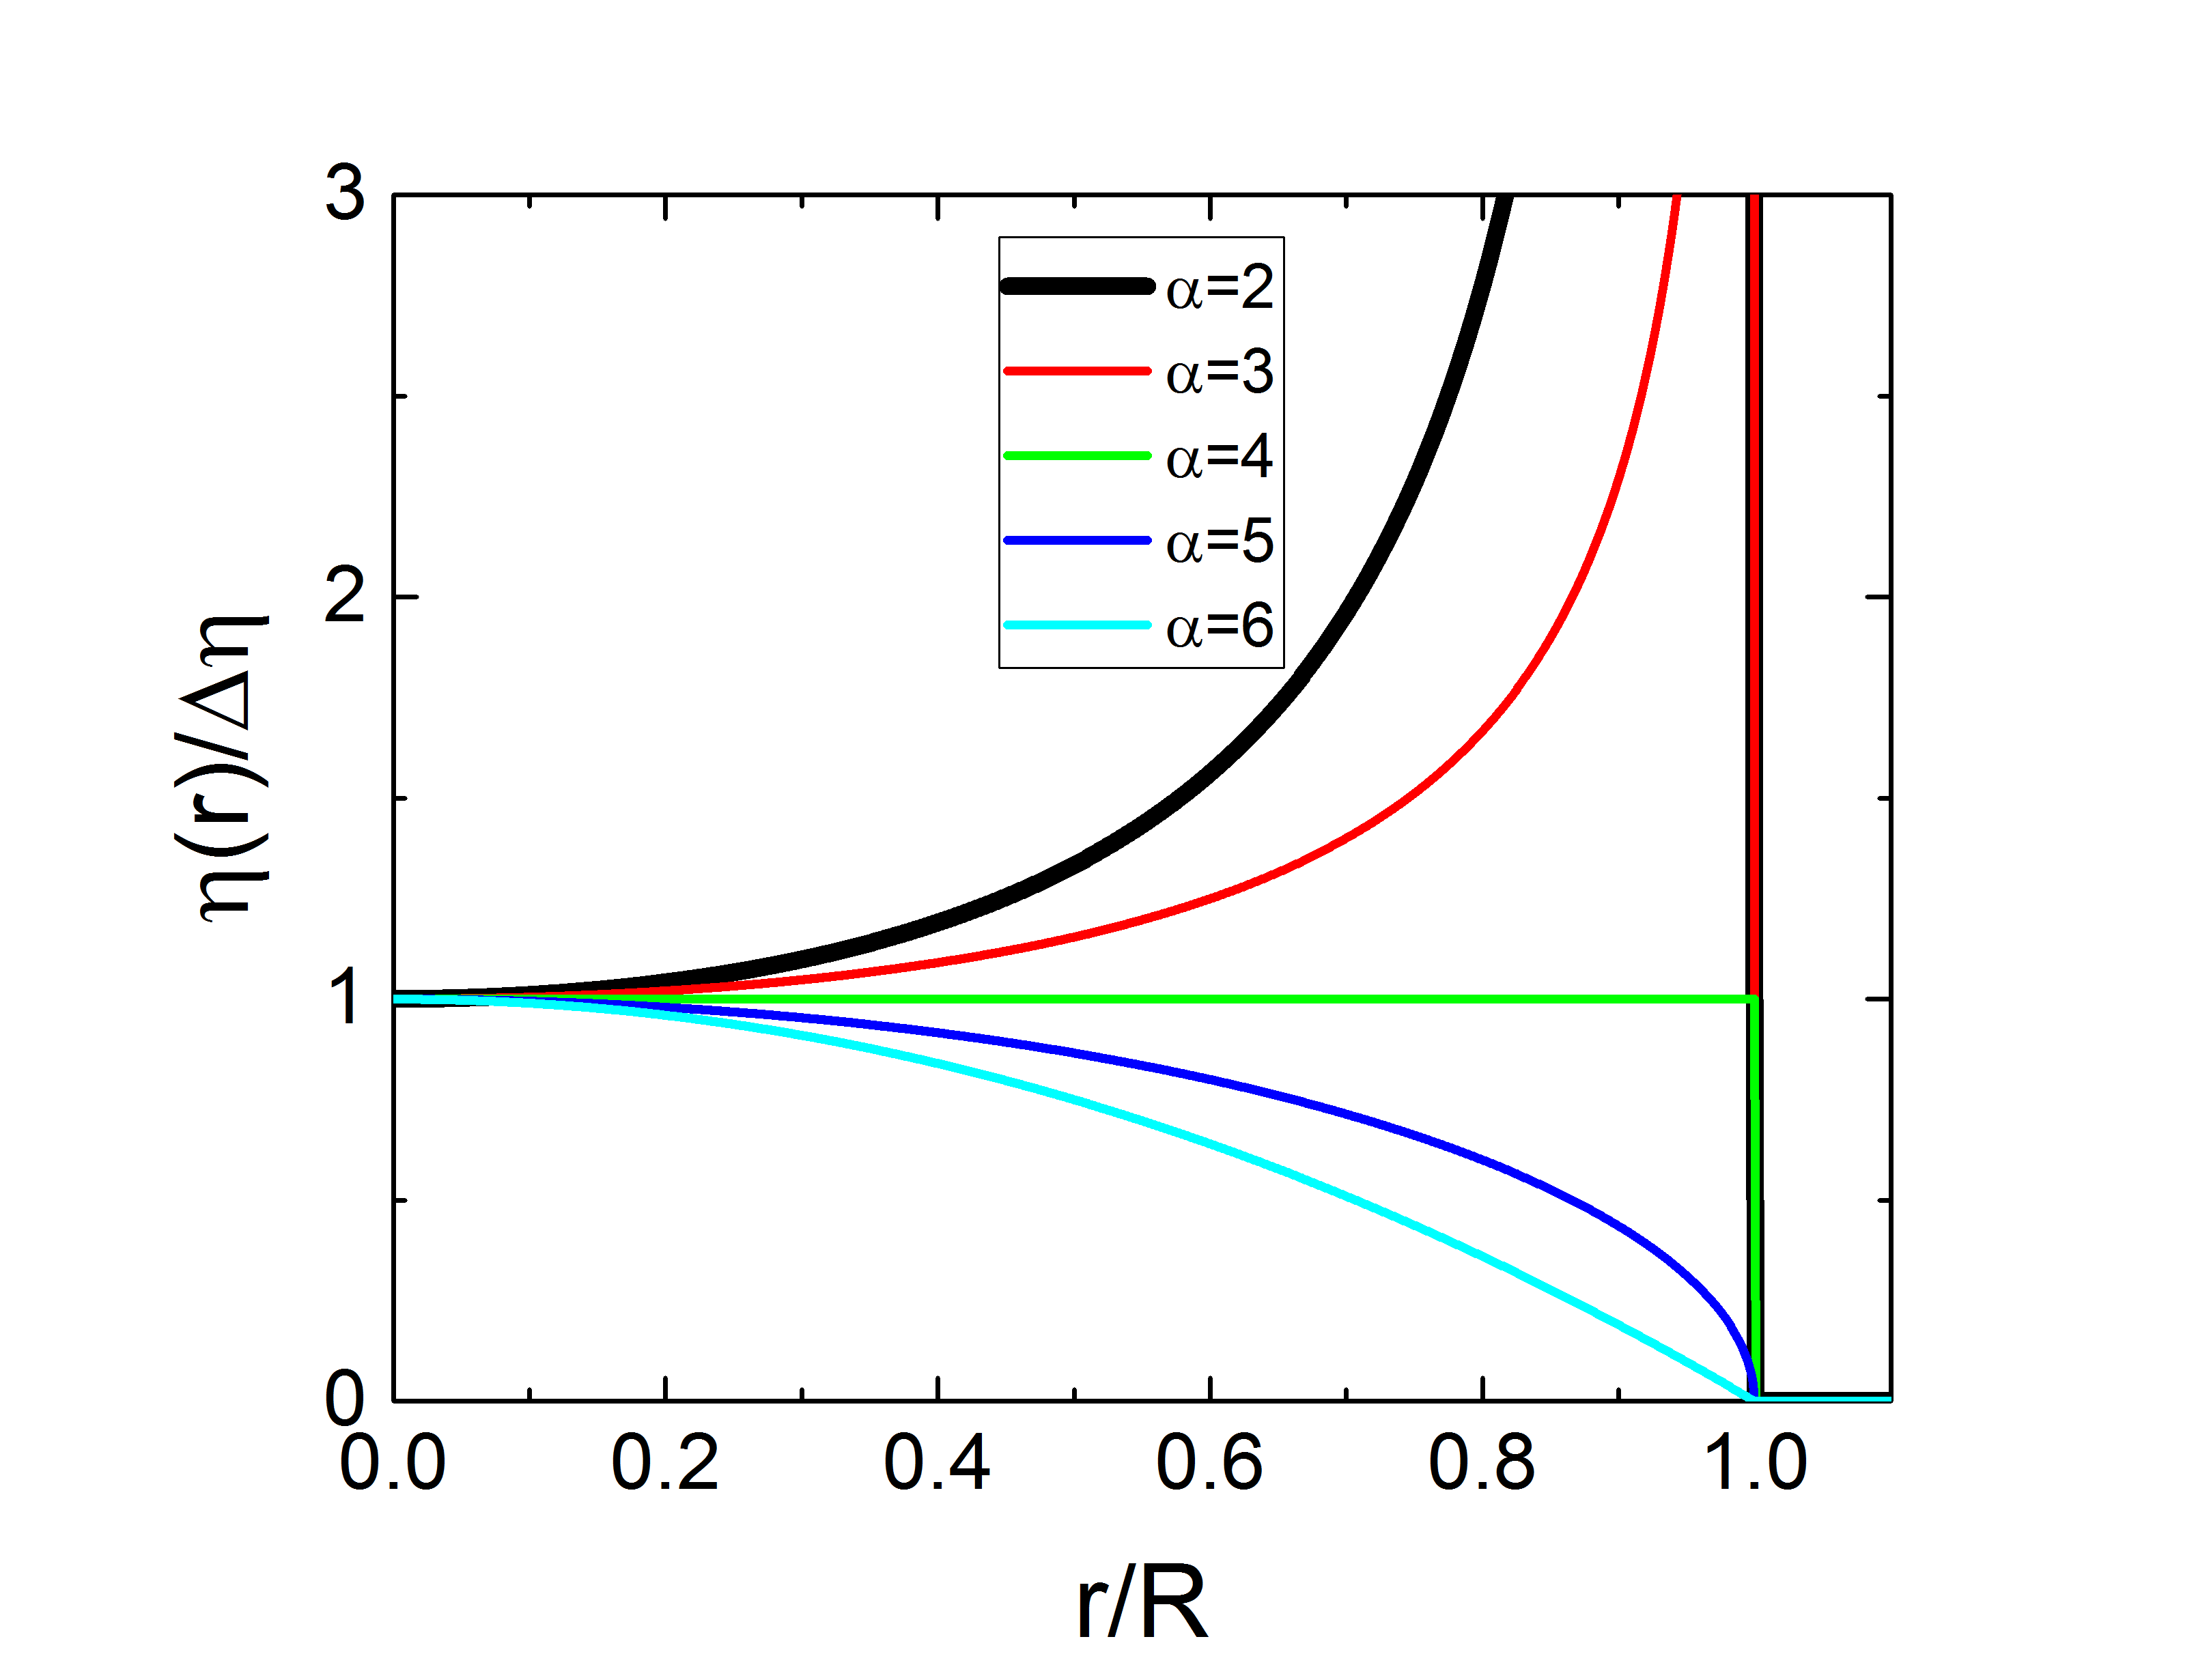
\includegraphics[width=0.48\textwidth]{Boucherprofile.png}}
\hfill
\subfigure[Radial profiles for several values of $\alpha$ with a normalised radial profile to assure $\alpha$-independent excess scattering length.
]{
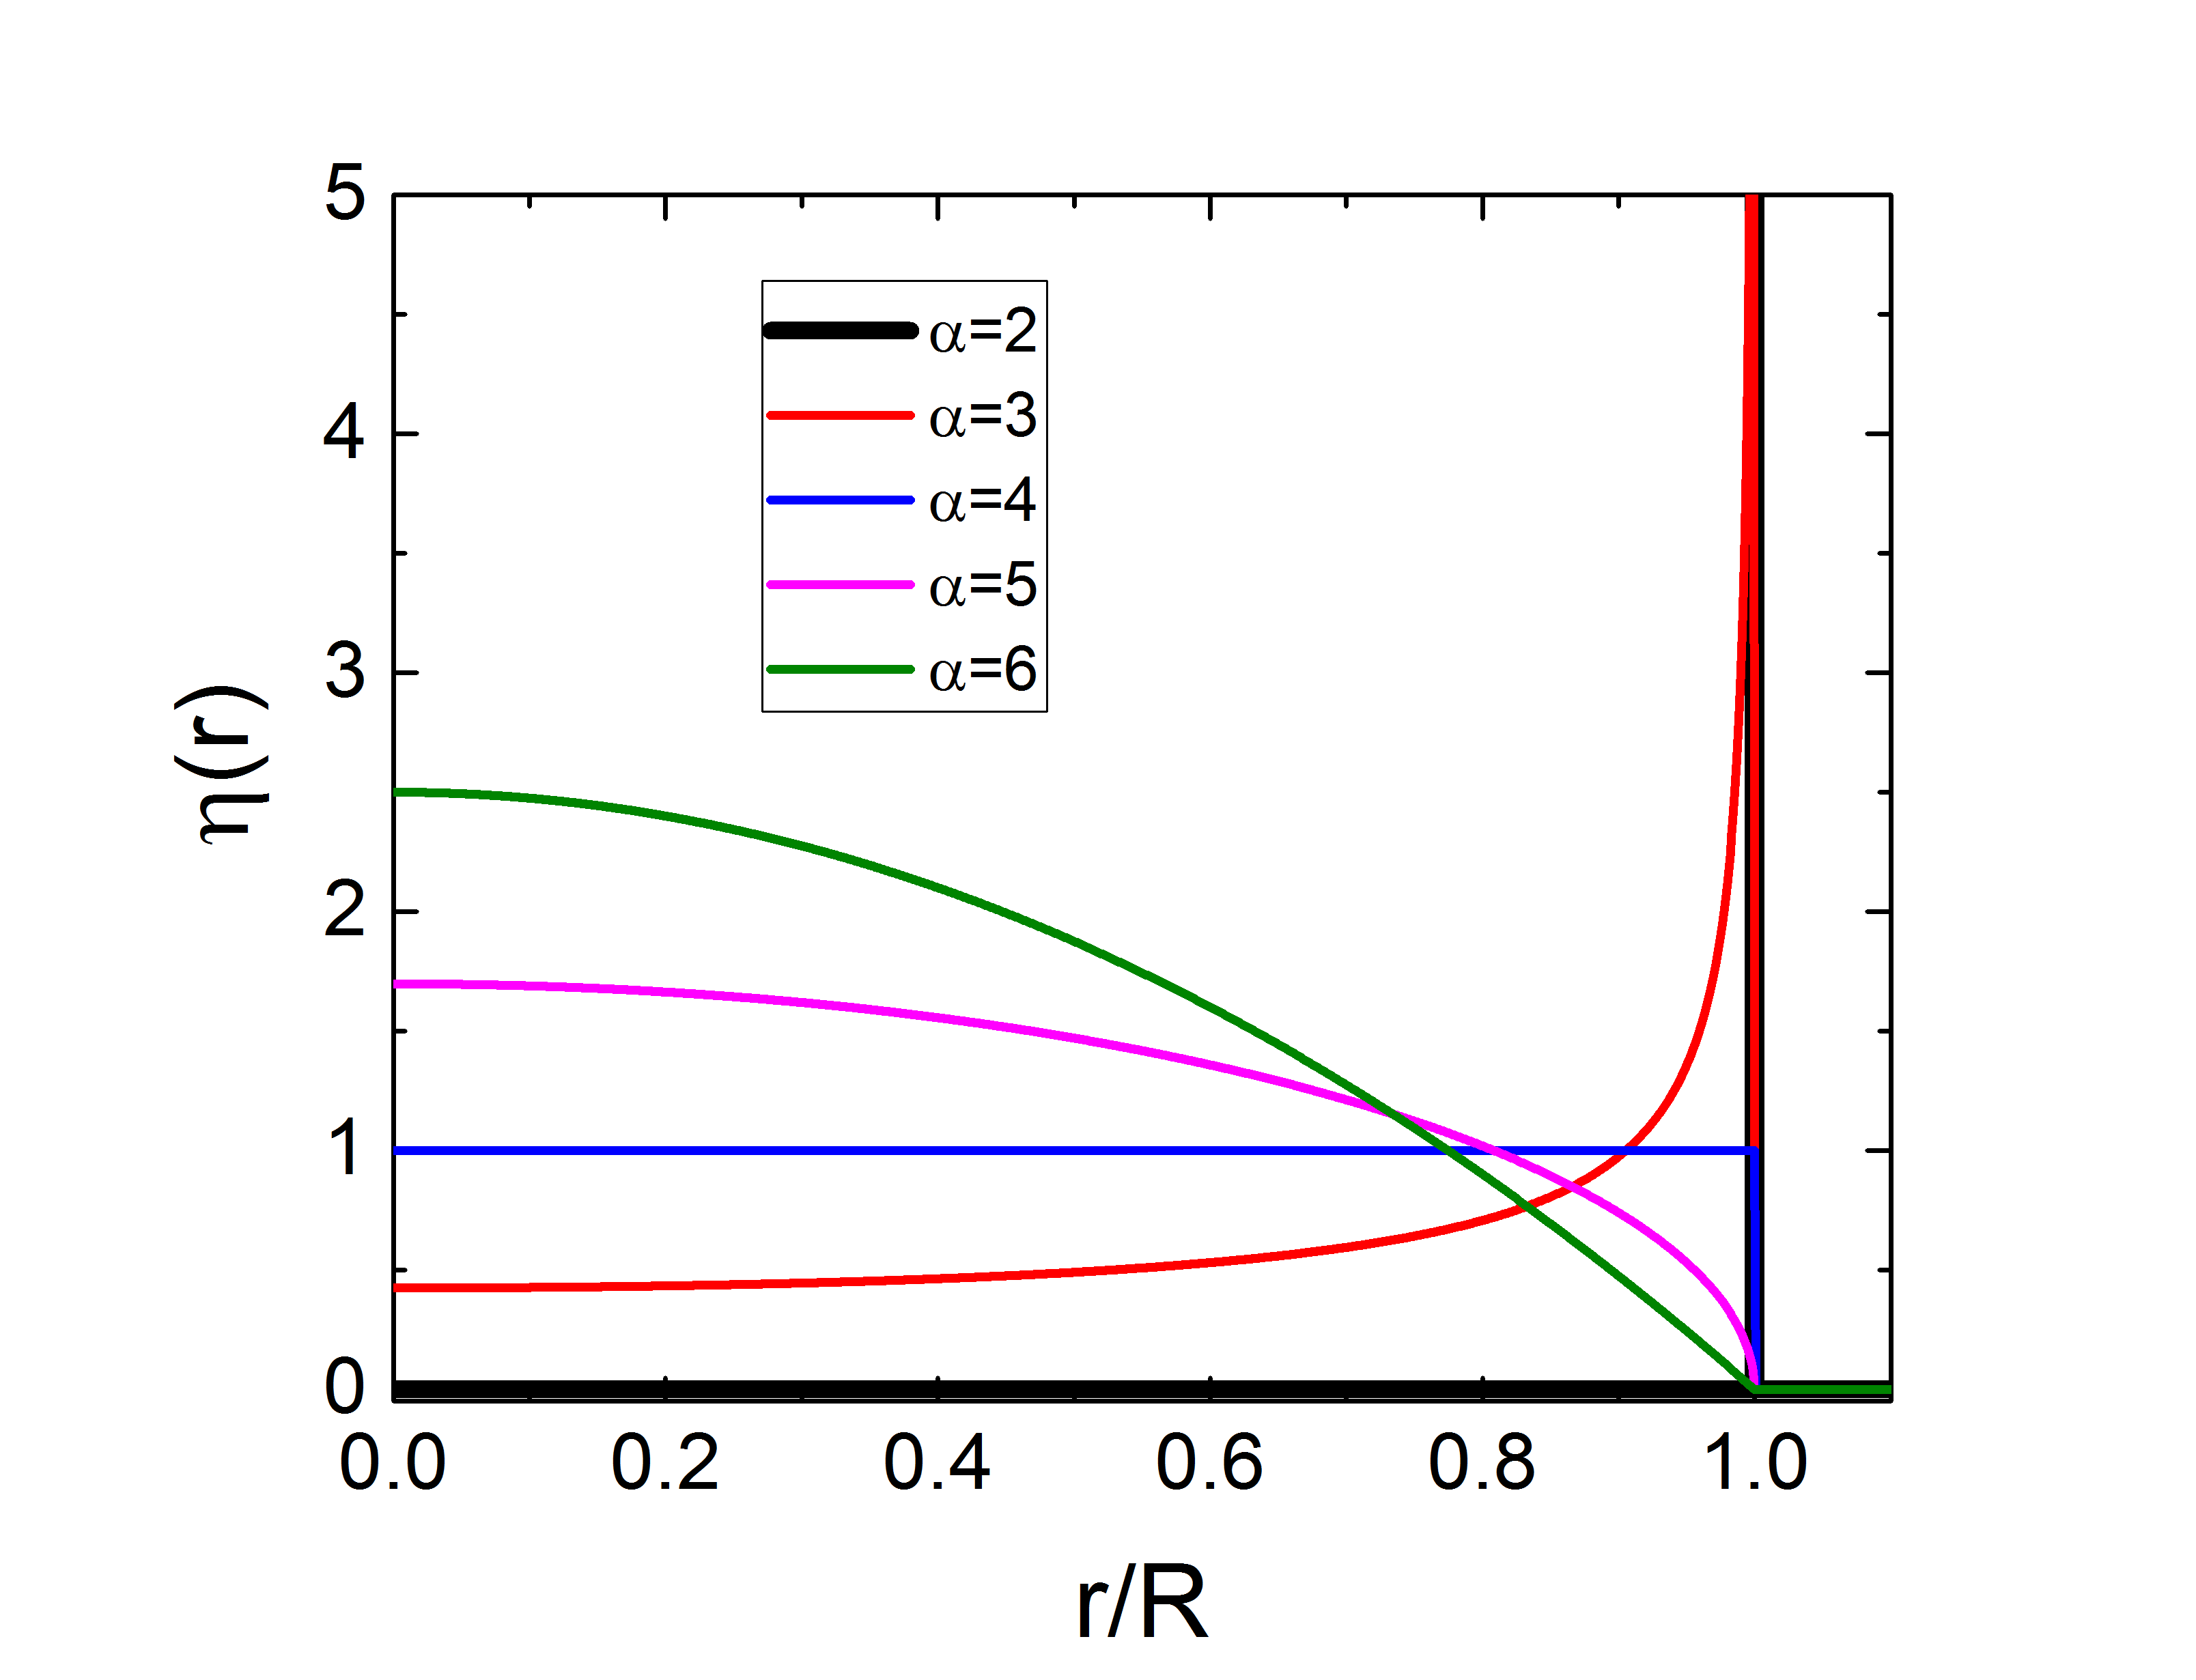
\includegraphics[width=0.48\textwidth]{Boucherprofile2.png}}
\end{center}
\caption{The two implemented case for the radial profiles according to Boucher \cite{Boucher1983}}
\label{fig:Boucherprofilea}
\end{figure}

Boucher  has described in \cite{Boucher1983} a simple analytical radial profile for which also the form factor can be calculated analytically. The radial profile is parameterized in a way that any potential law in the Porod regime can be obtained. The radial profile is defined by
\begin{align}
    \label{eq:profileBoucherSphere}
    \eta(r) &= \eta_0
    \begin{cases}
        \left[1-\left(\frac{r}{R}\right)^2 \right]^{\frac{\alpha}{2}-2} & \mbox{ for } r \leq R \\
        0 & \mbox{ for } r > R
    \end{cases}
\end{align}
The excess scattering $\beta$ of such a particle is
\BE
\beta = \int_0^R \eta(r) 4\pi r^2 \mathrm{d}r = \eta_0  R^3 \pi^{\frac{3}{2}} \frac{\Gamma\left(\frac{\alpha}{2}-1\right)}{\Gamma\left(\frac{\alpha+1}{2}\right)}
\EE
The input value $\Delta\eta$ for this profile is the scatter contrast at $r=0$, i.e.
\begin{align}
\eta_0&=\Delta\eta \qquad \mbox{(case \texttt{BoucherSphere})}
\label{eq:eta0BoucherSphere}
\end{align}
The special case of $\alpha=4$ corresponds to a homogeneous sphere with a scattering contrast $\Delta\eta$ for which the excess scattering length becomes $\beta_\mathrm{sp}=\Delta\eta \frac{4}{3}\pi R^3$.

 Also a second variant of the form factor has been implemented. In the second case the excess scattering length is normalised to the one of a homogeneous sphere with contrast $\Delta\eta$, so that the excess scattering length is for all $\alpha$ equal to $\beta_\mathrm{sp}=\Delta\eta \frac{4}{3}\pi R^3$. This is done by setting the contrast at $r=0$ in eq.\ \ref{eq:profileBoucherSphere} to
\begin{align}
\eta_0&=\Delta\eta \frac{4}{3\sqrt{\pi}} \frac{\Gamma\left(\frac{\alpha+1}{2}\right)}{\Gamma\left(\frac{\alpha}{2}-1\right)}  \qquad \mbox{(case \texttt{BoucherSphere2})}
\label{eq:eta0BoucherSphere2}
\end{align}
By this normalisation the excess scattering length is for all $\alpha$ equal to the one of a homogeneous sphere with a scattering contrast $\Delta\eta$, i.e. $\beta_\mathrm{sp}=\Delta\eta \frac{4}{3}\pi R^3$.

To get feeling which part of the spherical contributes most to the scattering ones can define
a fractional relative excess scattering length according to \cite{Boucher1983} which reads as
\begin{align}
Z(x) = & \frac{
            \int_{0}^{x}\! \left( 1-{\frac {{r}^{2}}{{R}^{2}}} \right) ^{\frac{\alpha}{2}-2} 4\pi\,{r}^{2}\,{\rm d}r
           }{
            \int_{0}^{R}\! \left( 1-{\frac {{r}^{2}}{{R}^{2}}} \right) ^{\frac{\alpha}{2}-2} 4\pi\,{r}^{2}\,{\rm d}r
           } \nonumber \\
  = & \frac{4}{3} \,{\frac {{x}^{3}\Gamma  \left(\frac{\alpha+1}{2} \right) }{\sqrt {\pi }
\Gamma  \left( \frac{\alpha}{2}-1 \right) {R}^{3}}
\;_2F_1\left(\frac{3}{2},-\frac{\alpha}{2}+2;\,\frac{5}{2};\,{\frac {{x}^{2}}{{R}^{2}}}\right)}
\end{align}
$Z(x)$ is the excess scattering of the sub-domain of the spherical particle ranging from $r=0$ to $r=x$ relative to the excess scattering of the whole particle. The derivative $Z'(x)$ then defines the fractional contribution of a sub-shell with radius $r=x$ and thickness $\textrm{d}x$  of the spherical particle compared to its total excess scattering length of the particle.

\begin{figure}[htb]
\begin{center}
\subfigure[Fractional relative excess scattering length $Z(x)$ for several $\alpha$.
]{
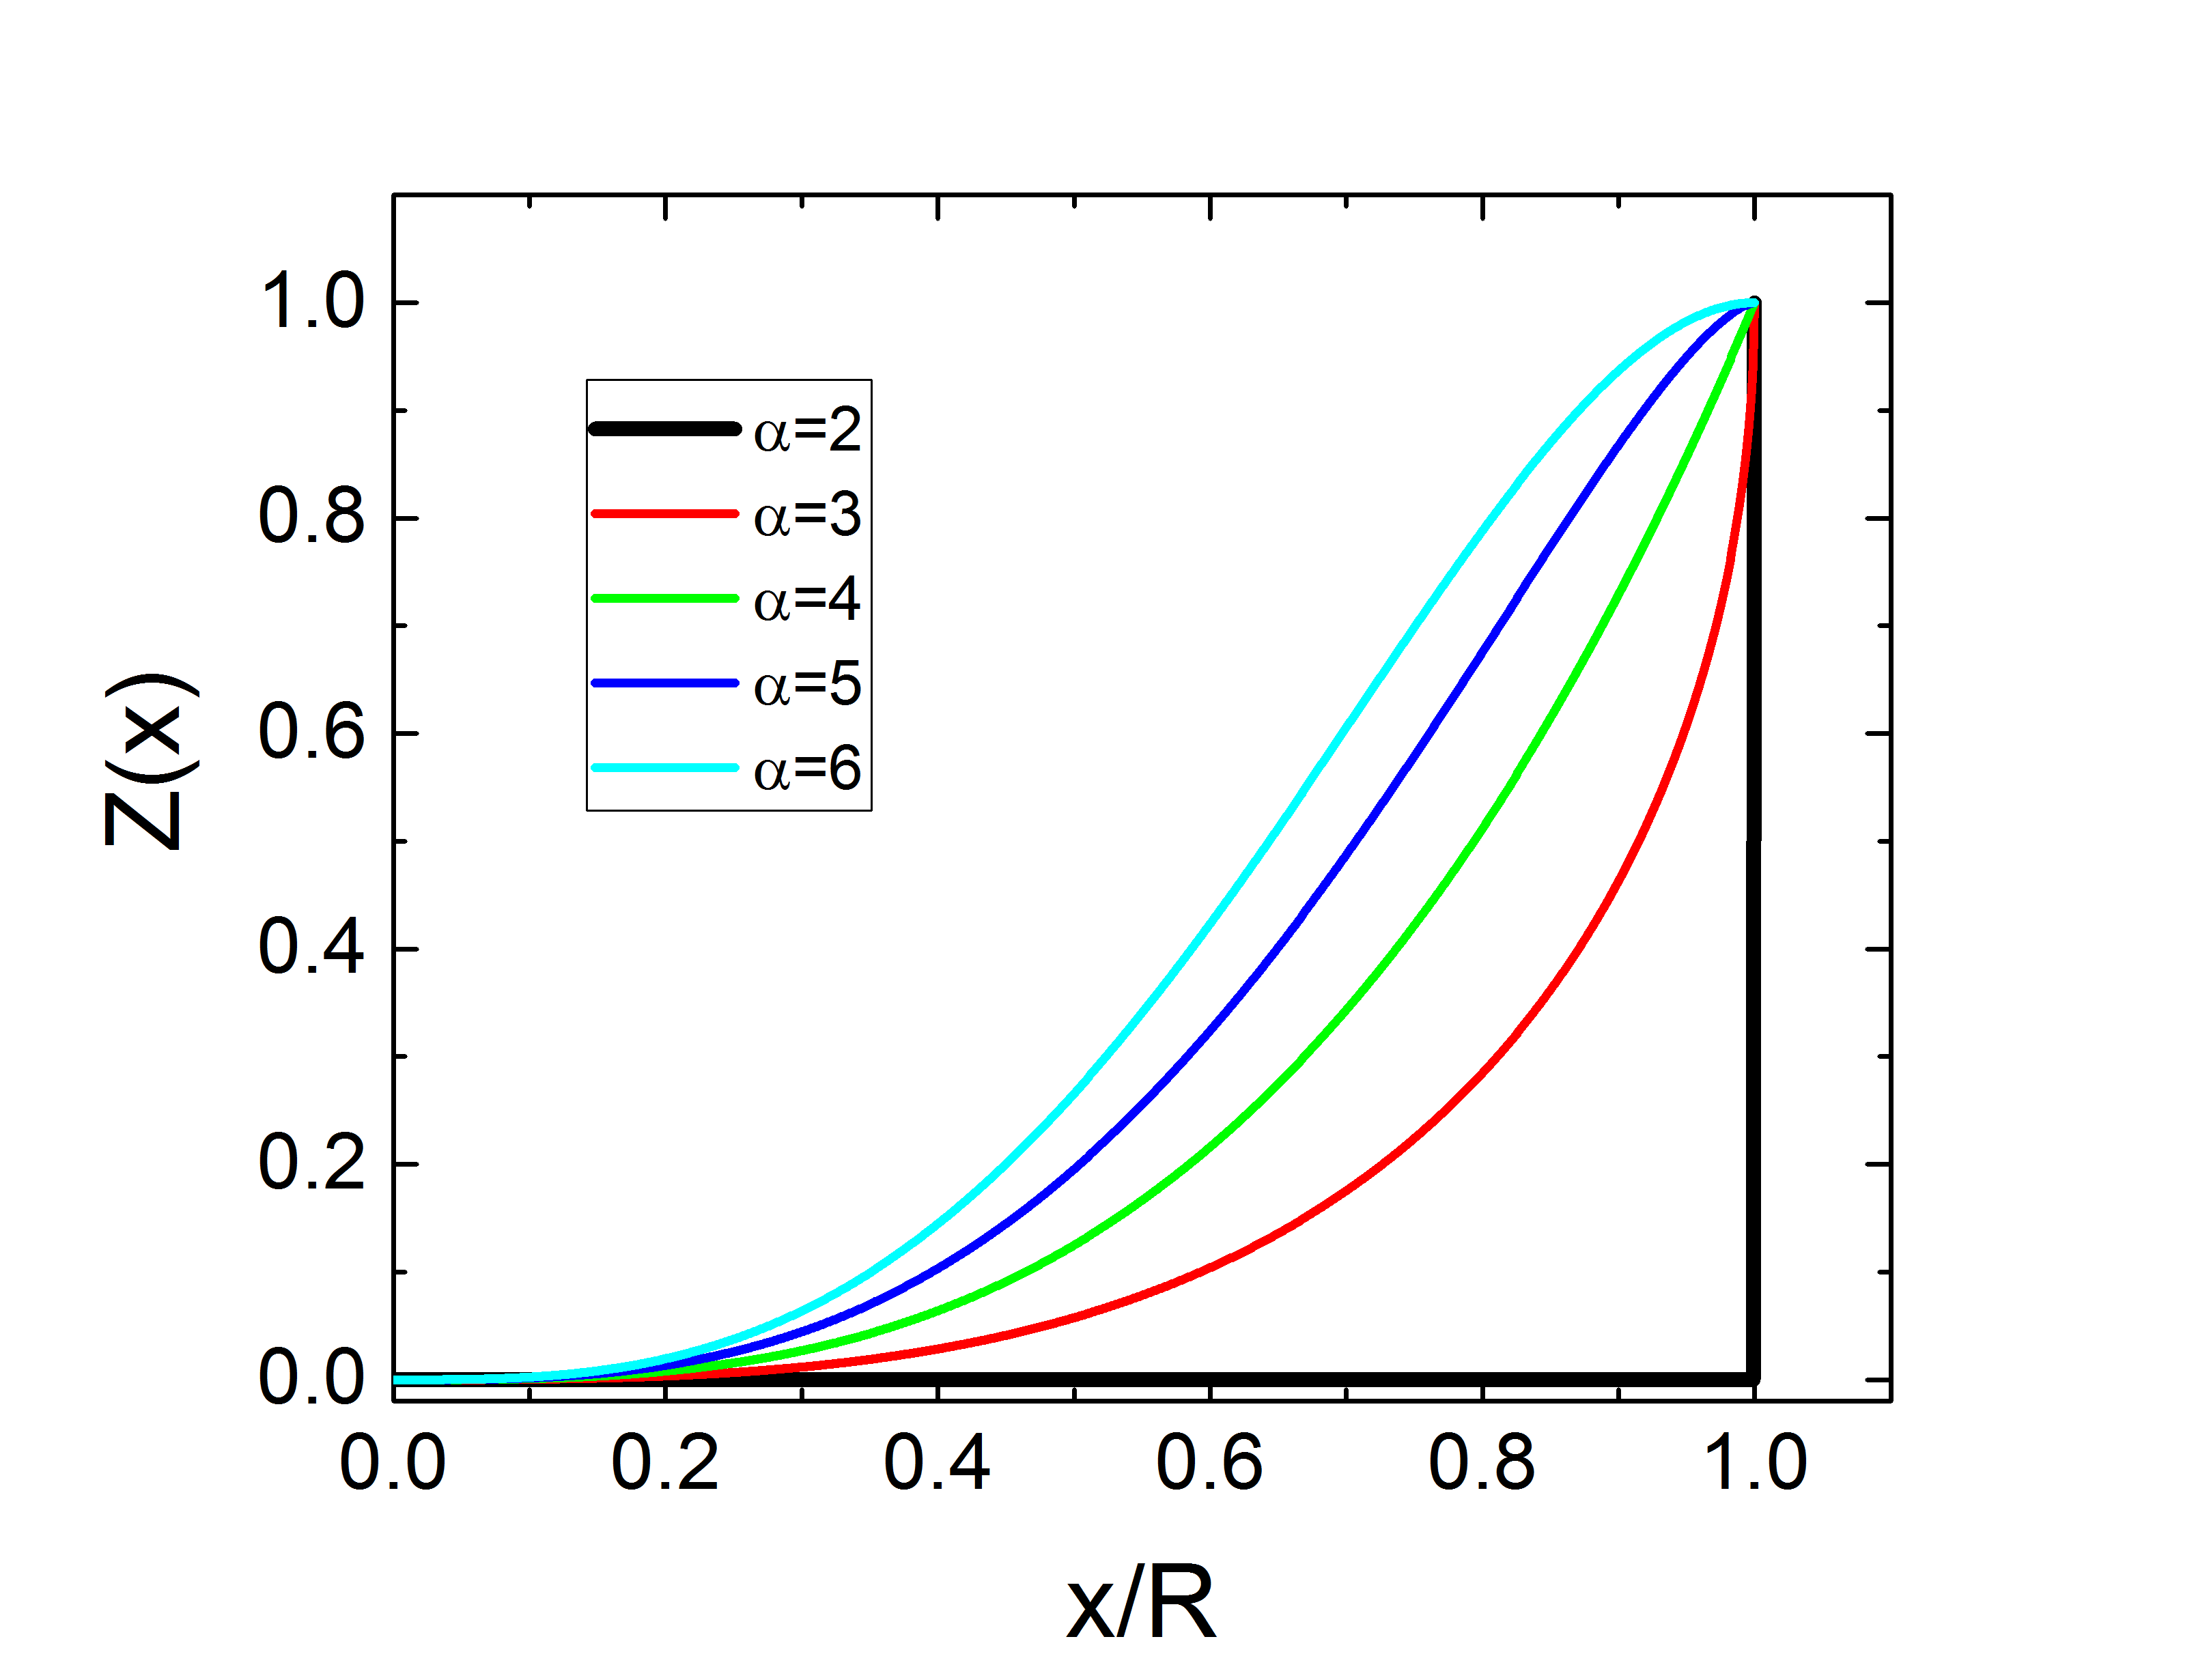
\includegraphics[width=0.48\textwidth]{BoucherZr.png}}
\hfill
\subfigure[Derivative of fractional relative excess scattering length $Z'(x)$ shows which part of the particle contributes how much to the excess scattering.
]{
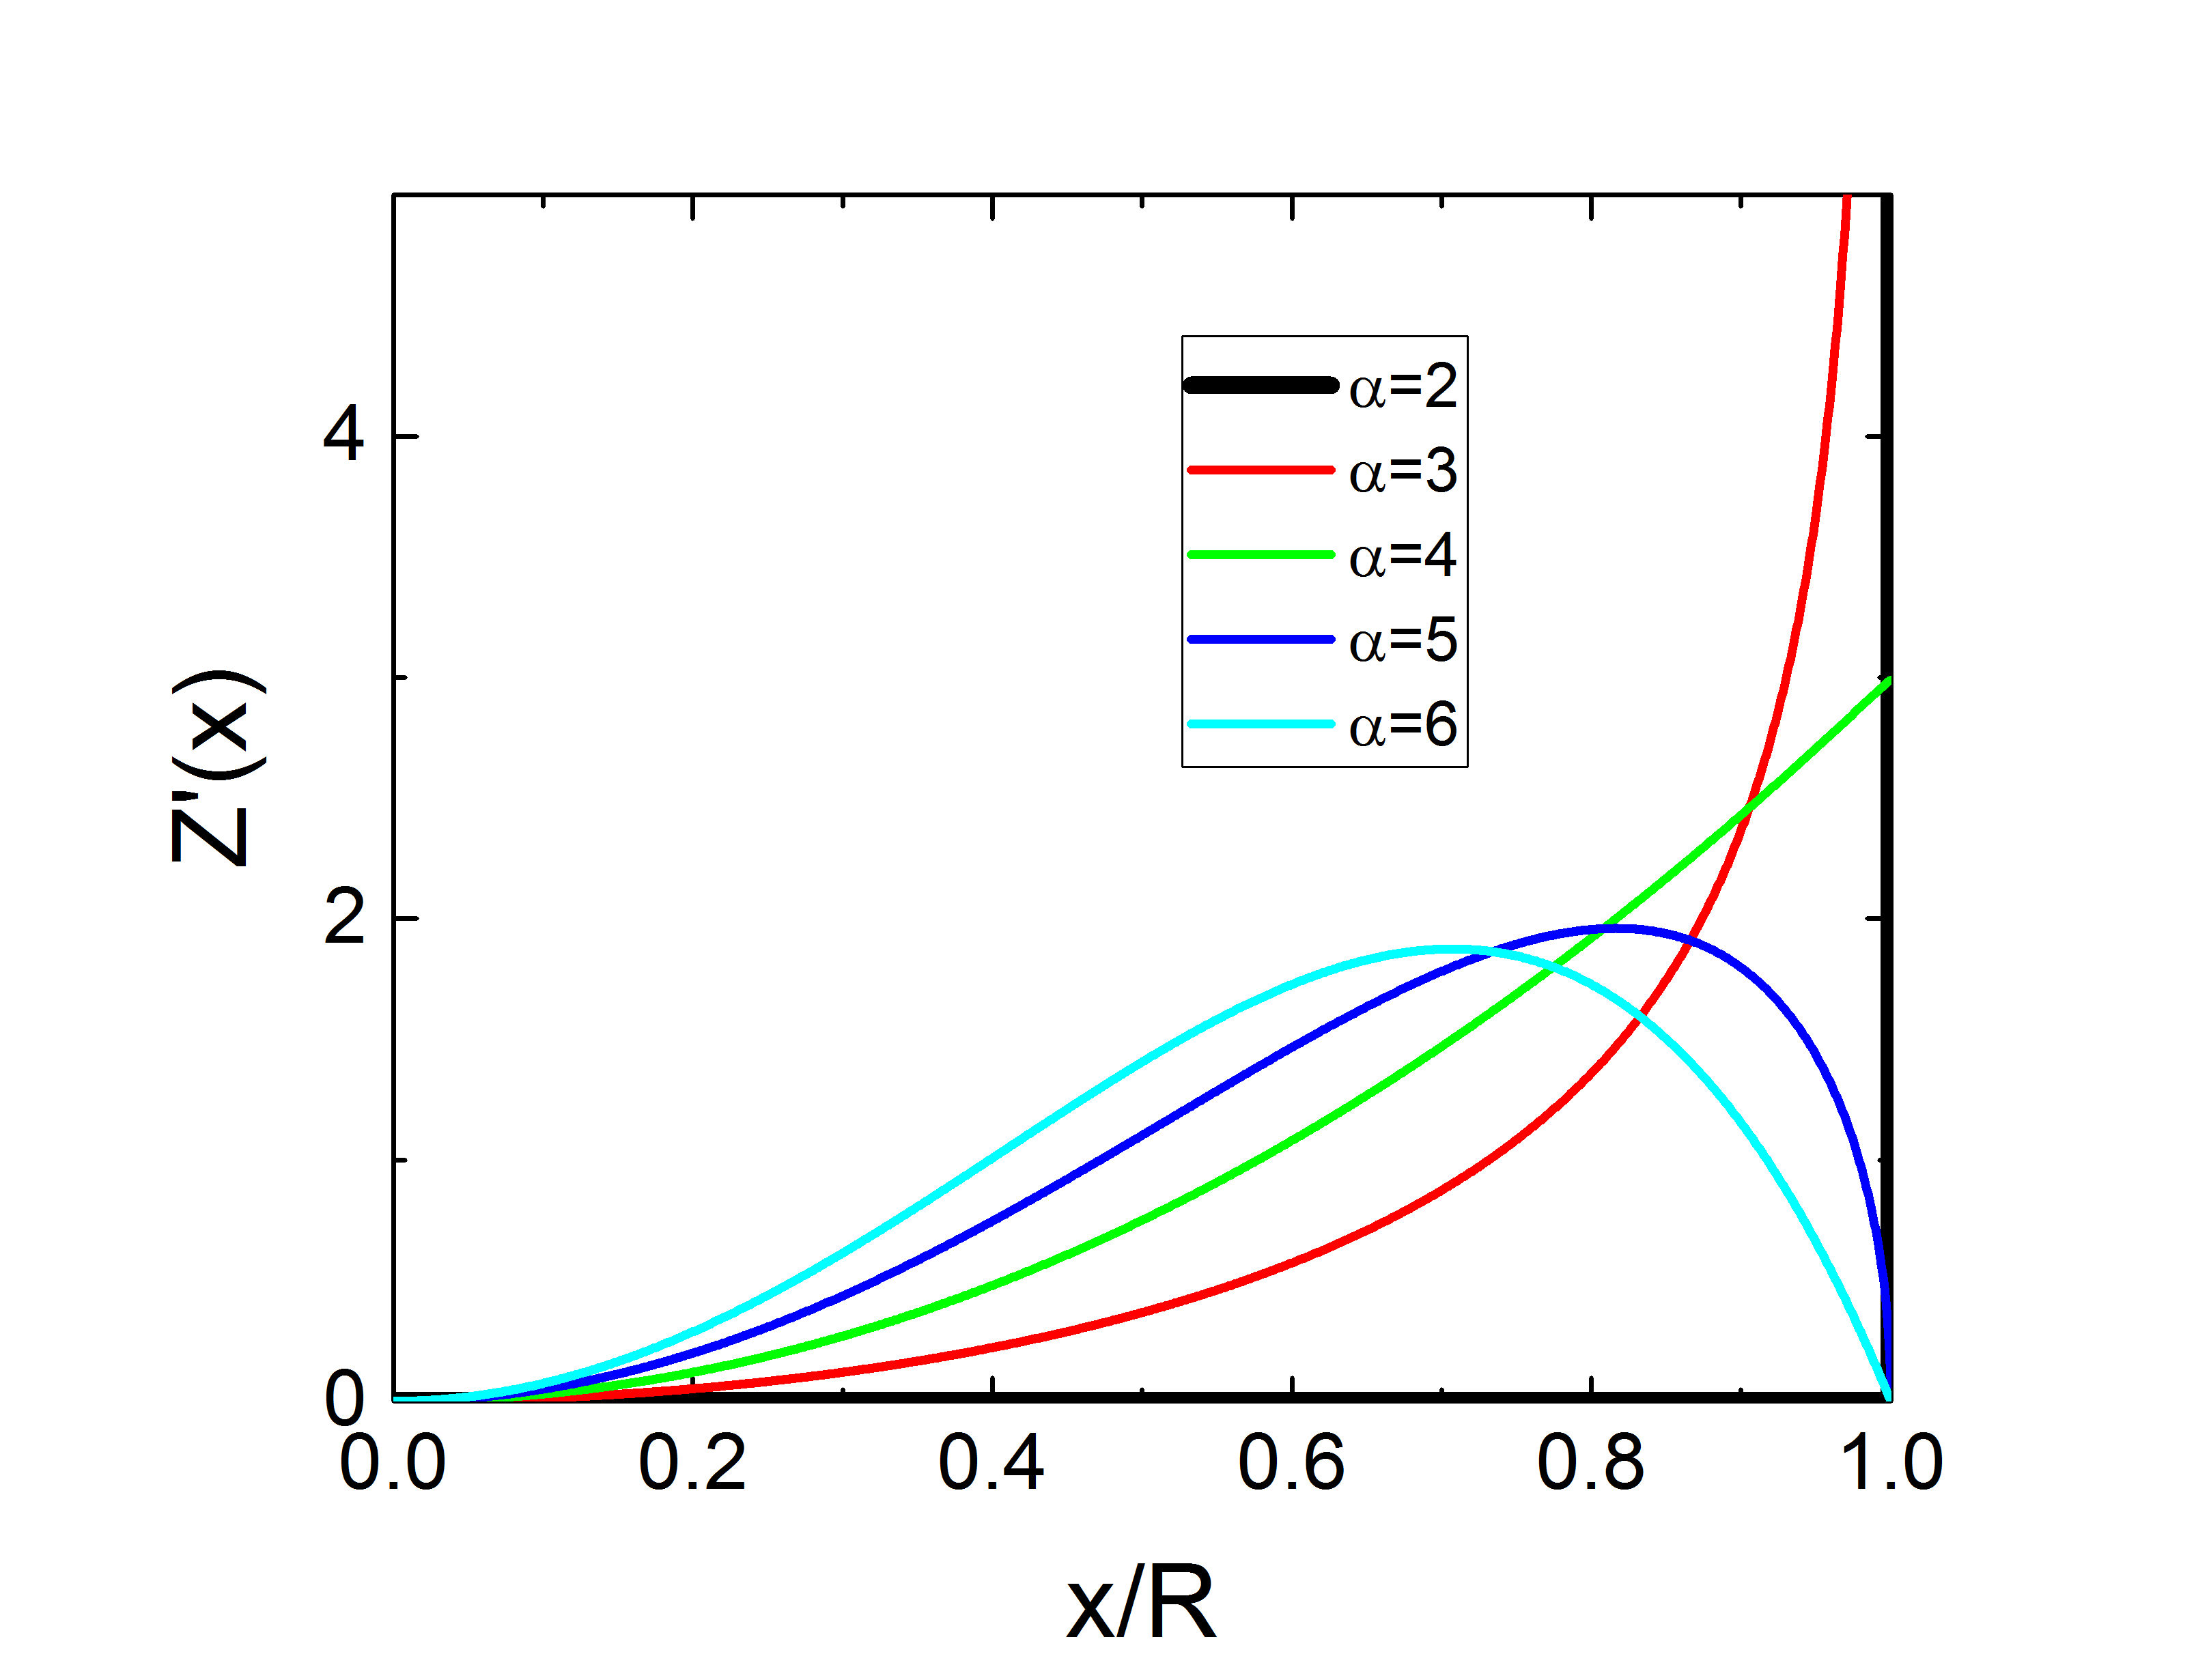
\includegraphics[width=0.48\textwidth]{BoucherZprime.png}}
\end{center}
\caption{For $\alpha=2$ all the scattering is caused by an infinitesimal thin outer shell of the particle where all the fractional excess scattering length is located.}
\label{fig:BoucherZr}
\end{figure}

The scattering amplitude for the radial profile in eq.\ \ref{eq:profileBoucherSphere} can be calculated as
\begin{align}
 F(Q) &= \int_0^R \eta(r) 4\pi r^2 \frac{\sin Qr}{Qr}\mathrm{d}r \nonumber \\
      &= \beta \left(\frac{2}{QR}\right)^{\frac{\alpha-1}{2}} J_{\frac{\alpha-1}{2}}(QR) \, \Gamma\left(\frac{\alpha+1}{2}\right) \nonumber \\
      &= \beta \;_0F_1\left(\frac{\alpha+1}{2};-\tfrac{(QR)^2}{4}\right)
\end{align}
making use of the fact that the bessel function can be expressed in terms of generalised hypergeometric functions $J_\alpha(x)=\frac{(\frac{x}{2})^\alpha}{\Gamma(\alpha+1)}  \;_0F_1 (\alpha+1; -\tfrac{x^2}{4})$. The scattering amplitude simplifies in case of $\alpha=4$ exactly the one of a homogenous spherical shell and in case of $\alpha=2$ to an infinitesimal thin spherical shell. For the scattering intensity $I(Q) = F^2(Q)$ we get in the Porod limit $Q\rightarrow\infty$
\BE
 \lim_{Q\rightarrow\infty} I(Q)= \lim_{Q\rightarrow\infty}  F^2(Q) =
 \beta^2 \frac{2^{\alpha-1}}{\pi} \Gamma^2\left(\frac{\alpha+1}{2}\right) \frac{1}{(QR)^\alpha}
\EE

\vspace{5mm}

\hspace{1pt}\\
\underline{Input Parameters for model \texttt{BoucherSphere} and \texttt{Boucher profile}:}\\
\begin{description}
\item[\texttt{R}] radius $R$
\item[\texttt{alpha}] shape parameter of the profile $\alpha$, which is also equal to the potential law at large $Q$-values
\item[\texttt{Delta\_eta}] scattering length density at $r=0$, $\Delta\eta=\eta(r=0)$
\end{description}

\noindent\underline{Note for model \texttt{BoucherSphere} and \texttt{Boucher profile}:}
\begin{itemize}
\item For $\alpha<4$ the scattering length density profile has a pole at $r=R$
\item For $\alpha \leq 2$ the excess scattering length of the overall particle diverges and are therefore forbidden values.
\end{itemize}

\hspace{1pt}\\
\underline{Input Parameters for model \texttt{BoucherSphere2} and \texttt{Boucher profile2}:}\\
\begin{description}
\item[\texttt{R}] radius $R$
\item[\texttt{alpha}] shape parameter of the profile $\alpha$, which is also equal to the potential law at large $Q$-values
\item[\texttt{Delta\_eta}] average scattering length density so that the excess scattering length corresponds to that one of a homogeneous sphere with contrast $\Delta\eta$
\end{description}

\noindent\underline{Note for model \texttt{BoucherSphere2} and \texttt{Boucher profile}:}
\begin{itemize}
\item For $\alpha<4$ the scattering length density profile has a pole at $r=R$
\item There is no restriction for the input values of $\alpha$ in the form factor but in the profile, which only allows values for $\alpha>2$.  $\alpha$-values below 2 do not have a standard physical interpretation.
\end{itemize}

\begin{figure}[htb]
\begin{center}
\subfigure[Scattering curves of \texttt{BoucherSpheres} for sevaral $\alpha$ with a narrow LogNormal size distribution with $\sigma=0.1$. As the excess scattering length diverges for $\alpha\leq 2$ these values are not allowed.]{
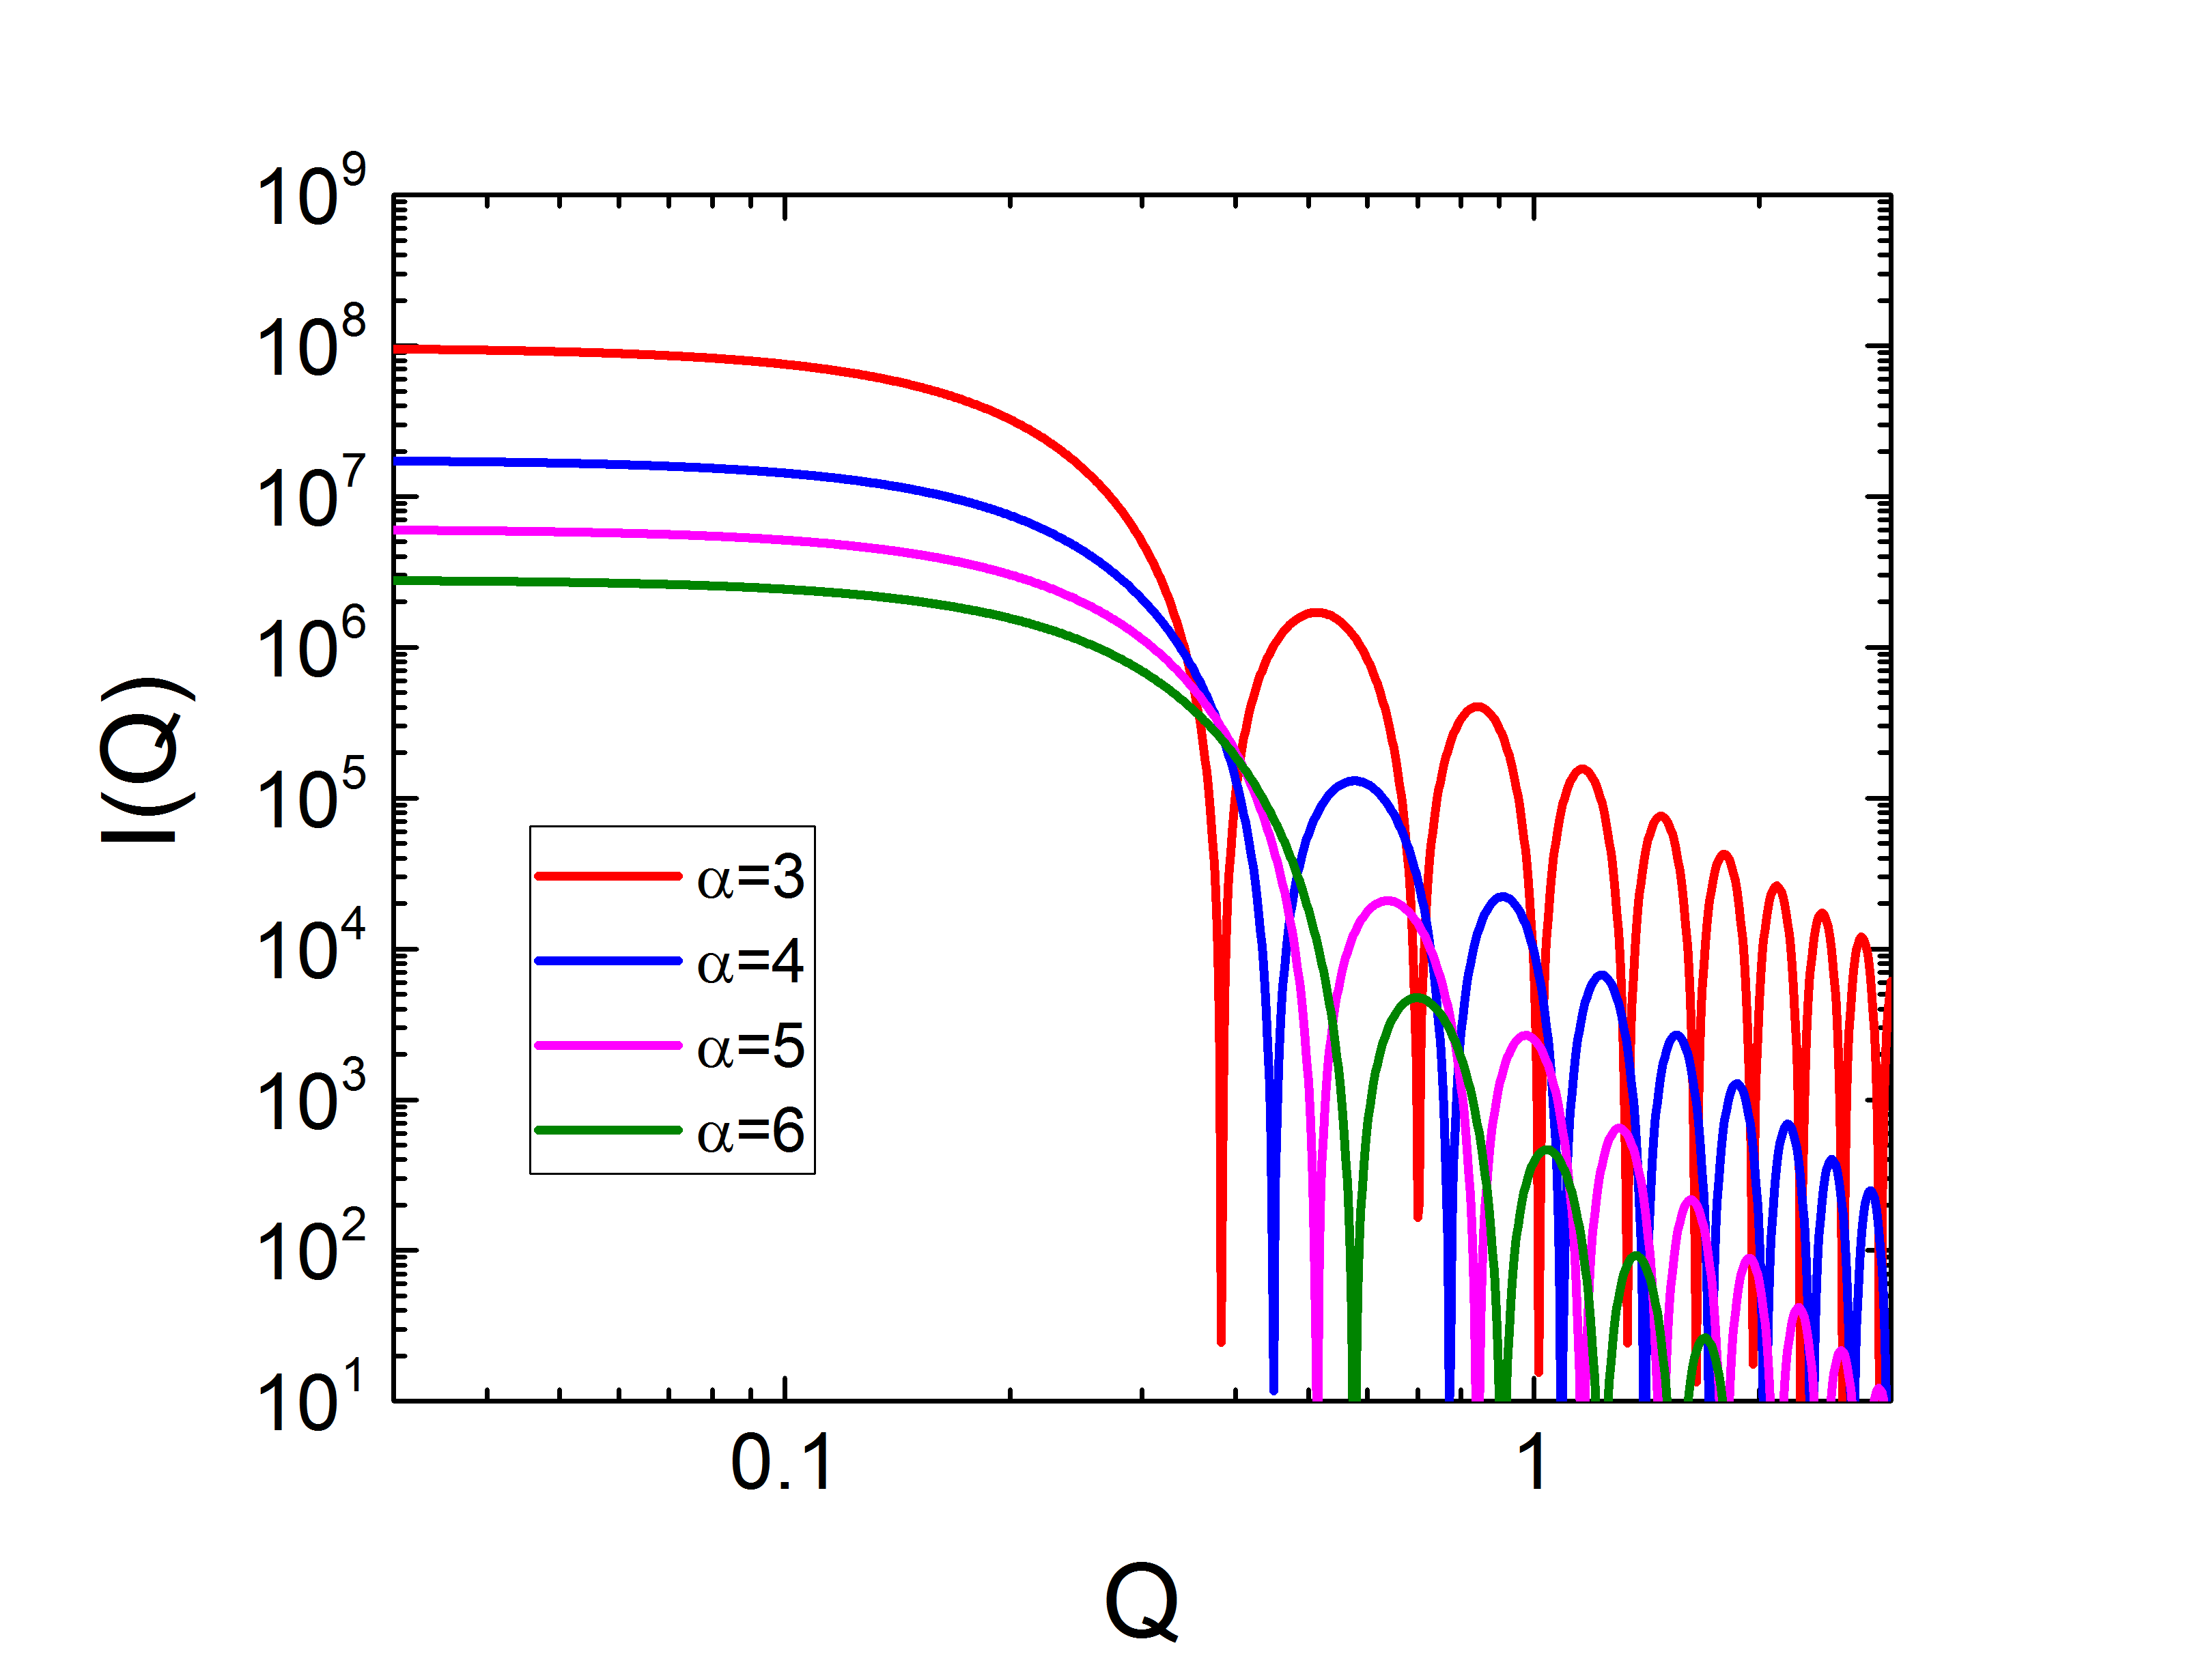
\includegraphics[width=0.48\textwidth]{BoucherSphereI(Q).png}}
\hfill
\subfigure[Scattering curves of \texttt{BoucherSpheres2} for sevaral $\alpha$ with a narrow LogNormal size distribution with $\sigma=0.1$.]{
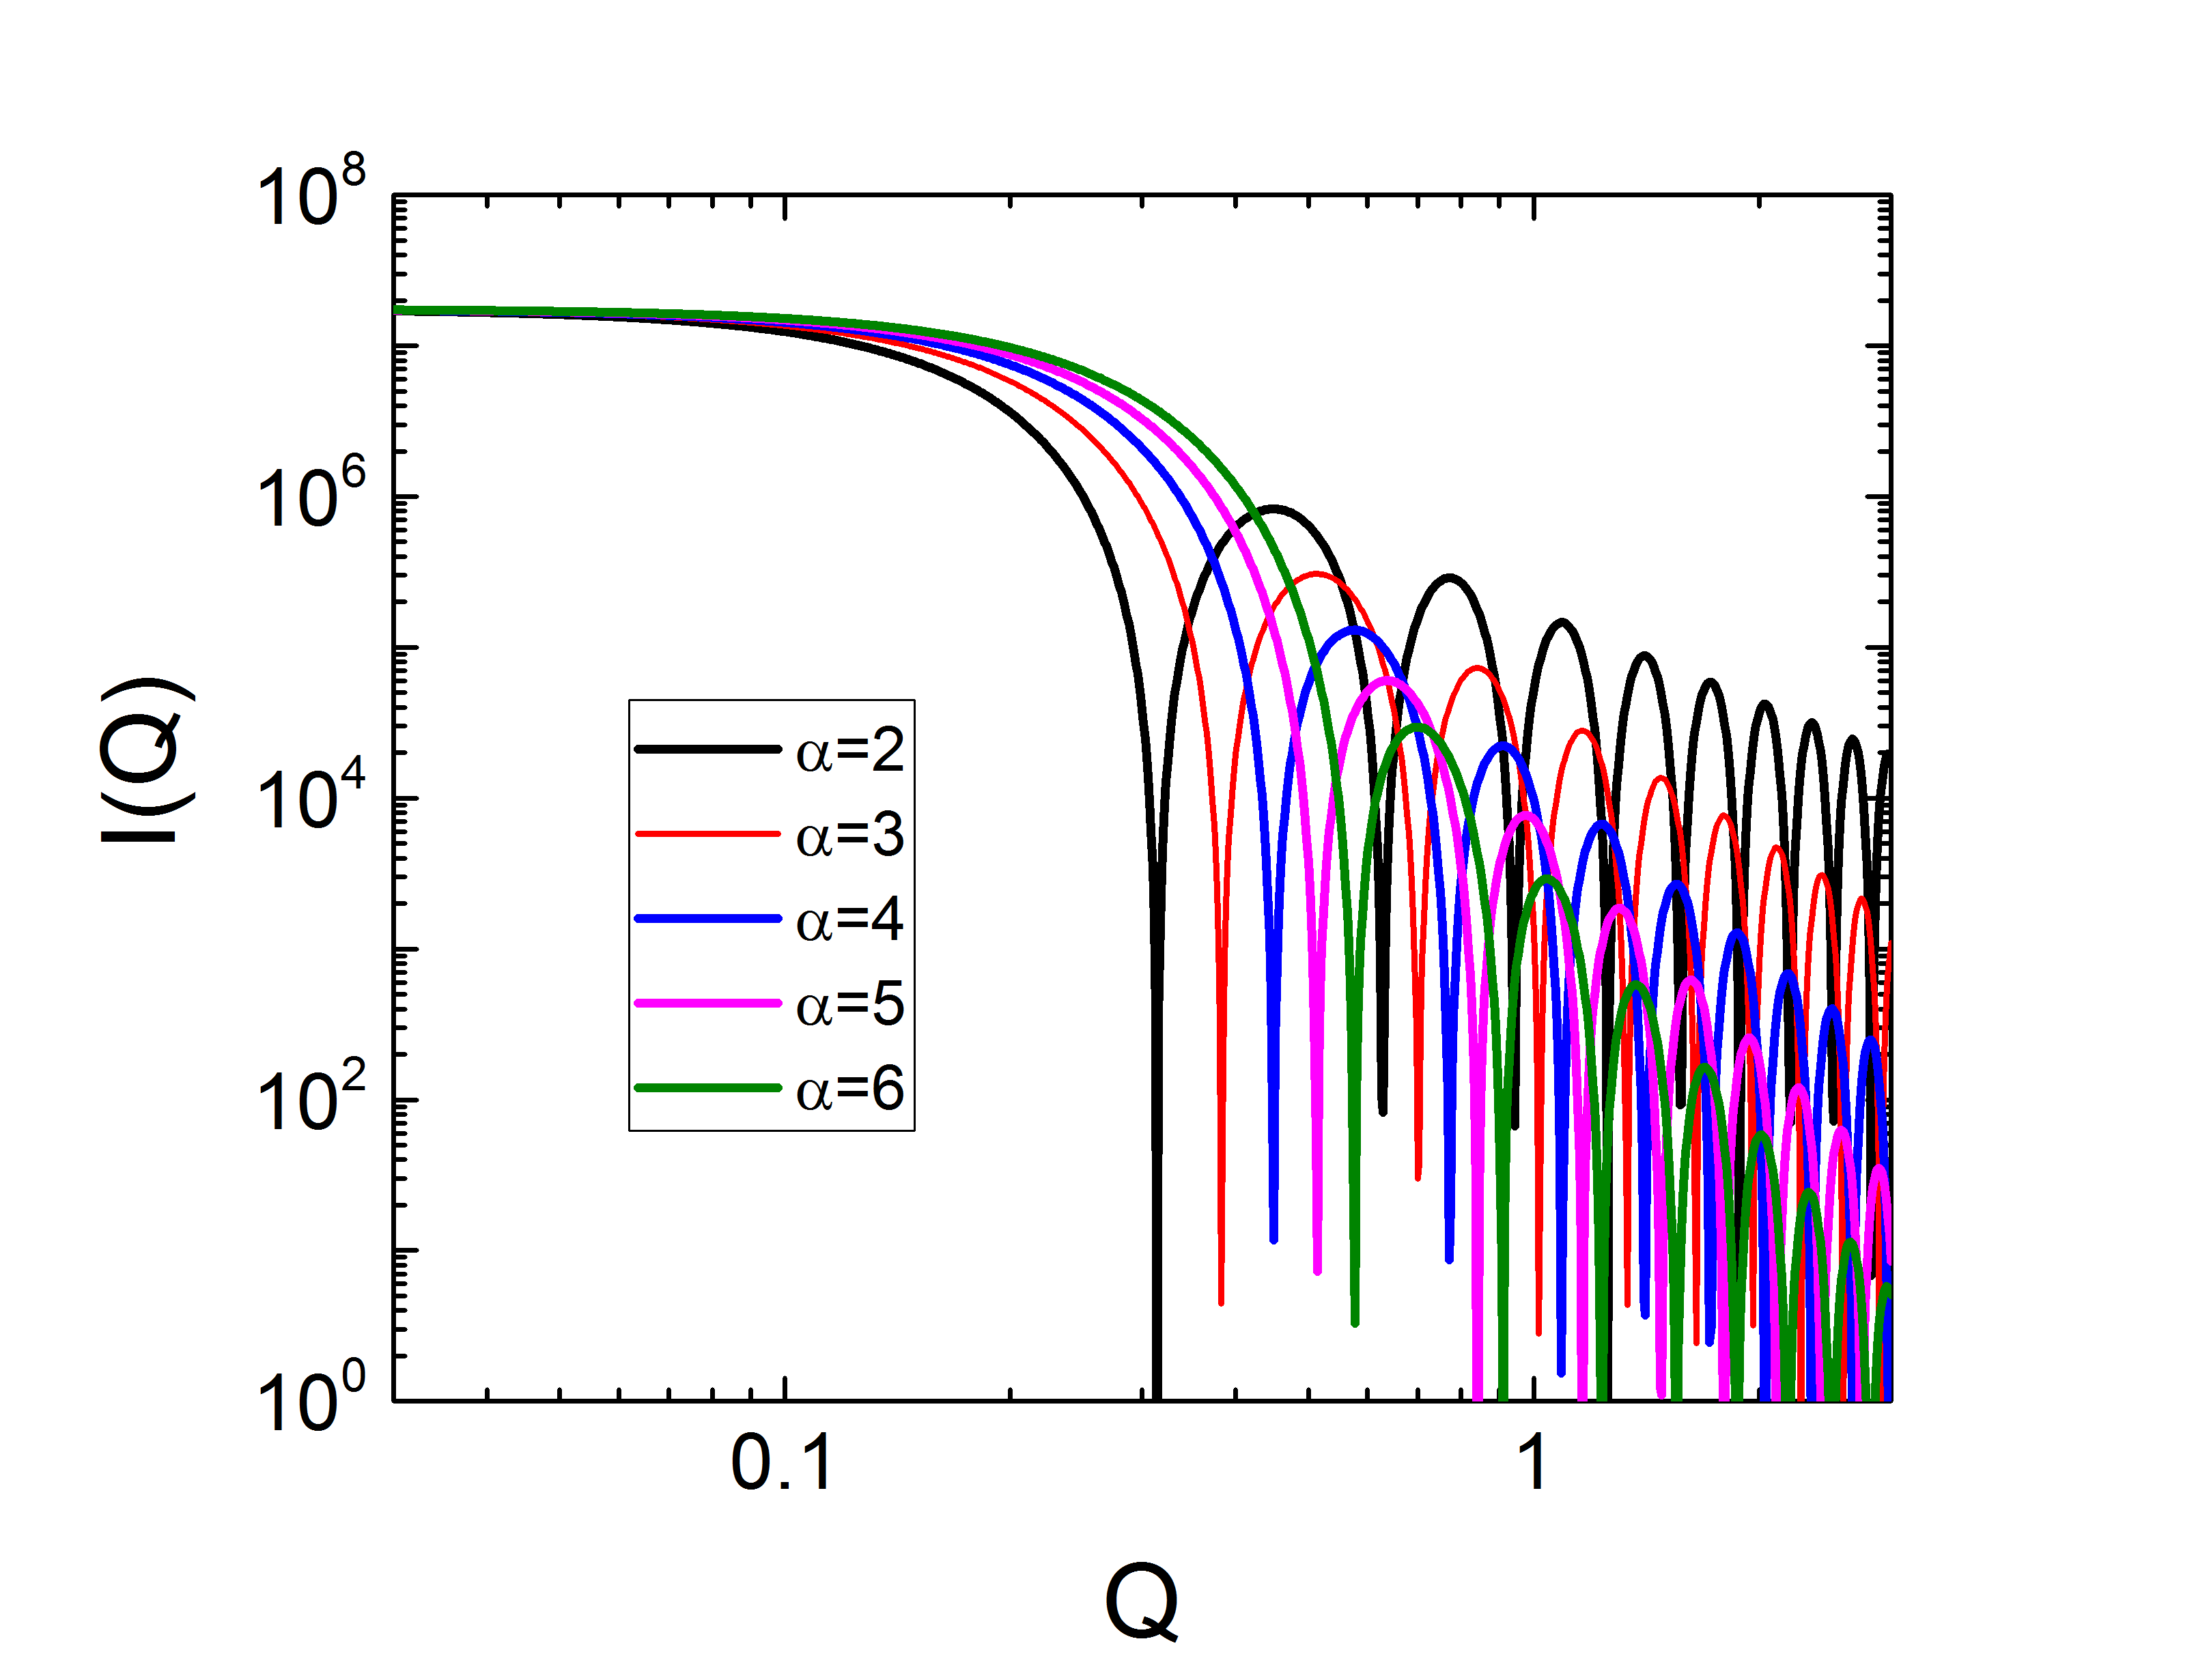
\includegraphics[width=0.48\textwidth]{BoucherSphere2I(Q).png}}
\end{center}
\caption{Scattering curves for the form factors \texttt{BoucherSpheres} and \texttt{BoucherSpheres2}.}
\label{fig:BoucherIQ}
\end{figure} 